\documentclass[]{ctexbook}
\usepackage{lmodern}
\usepackage{amssymb,amsmath}
\usepackage{ifxetex,ifluatex}
\usepackage{fixltx2e} % provides \textsubscript
\ifnum 0\ifxetex 1\fi\ifluatex 1\fi=0 % if pdftex
  \usepackage[T1]{fontenc}
  \usepackage[utf8]{inputenc}
\else % if luatex or xelatex
  \ifxetex
    \usepackage{xltxtra,xunicode}
  \else
    \usepackage{fontspec}
  \fi
  \defaultfontfeatures{Ligatures=TeX,Scale=MatchLowercase}
\fi
% use upquote if available, for straight quotes in verbatim environments
\IfFileExists{upquote.sty}{\usepackage{upquote}}{}
% use microtype if available
\IfFileExists{microtype.sty}{%
\usepackage{microtype}
\UseMicrotypeSet[protrusion]{basicmath} % disable protrusion for tt fonts
}{}
\usepackage[a4paper,tmargin=2.5cm,bmargin=2.5cm,lmargin=3.5cm,rmargin=2.5cm]{geometry}
\usepackage[unicode=true]{hyperref}
\PassOptionsToPackage{usenames,dvipsnames}{color} % color is loaded by hyperref
\hypersetup{
            pdftitle={肠道菌群研究二十年·大数据},
            pdfauthor={热心肠研究院},
            colorlinks=true,
            linkcolor=Maroon,
            citecolor=Blue,
            urlcolor=Blue,
            breaklinks=true}
\urlstyle{same}  % don't use monospace font for urls
\usepackage{natbib}
\bibliographystyle{apalike}
\usepackage{color}
\usepackage{fancyvrb}
\newcommand{\VerbBar}{|}
\newcommand{\VERB}{\Verb[commandchars=\\\{\}]}
\DefineVerbatimEnvironment{Highlighting}{Verbatim}{commandchars=\\\{\}}
% Add ',fontsize=\small' for more characters per line
\usepackage{framed}
\definecolor{shadecolor}{RGB}{248,248,248}
\newenvironment{Shaded}{\begin{snugshade}}{\end{snugshade}}
\newcommand{\AlertTok}[1]{\textcolor[rgb]{0.94,0.16,0.16}{#1}}
\newcommand{\AnnotationTok}[1]{\textcolor[rgb]{0.56,0.35,0.01}{\textbf{\textit{#1}}}}
\newcommand{\AttributeTok}[1]{\textcolor[rgb]{0.77,0.63,0.00}{#1}}
\newcommand{\BaseNTok}[1]{\textcolor[rgb]{0.00,0.00,0.81}{#1}}
\newcommand{\BuiltInTok}[1]{#1}
\newcommand{\CharTok}[1]{\textcolor[rgb]{0.31,0.60,0.02}{#1}}
\newcommand{\CommentTok}[1]{\textcolor[rgb]{0.56,0.35,0.01}{\textit{#1}}}
\newcommand{\CommentVarTok}[1]{\textcolor[rgb]{0.56,0.35,0.01}{\textbf{\textit{#1}}}}
\newcommand{\ConstantTok}[1]{\textcolor[rgb]{0.00,0.00,0.00}{#1}}
\newcommand{\ControlFlowTok}[1]{\textcolor[rgb]{0.13,0.29,0.53}{\textbf{#1}}}
\newcommand{\DataTypeTok}[1]{\textcolor[rgb]{0.13,0.29,0.53}{#1}}
\newcommand{\DecValTok}[1]{\textcolor[rgb]{0.00,0.00,0.81}{#1}}
\newcommand{\DocumentationTok}[1]{\textcolor[rgb]{0.56,0.35,0.01}{\textbf{\textit{#1}}}}
\newcommand{\ErrorTok}[1]{\textcolor[rgb]{0.64,0.00,0.00}{\textbf{#1}}}
\newcommand{\ExtensionTok}[1]{#1}
\newcommand{\FloatTok}[1]{\textcolor[rgb]{0.00,0.00,0.81}{#1}}
\newcommand{\FunctionTok}[1]{\textcolor[rgb]{0.00,0.00,0.00}{#1}}
\newcommand{\ImportTok}[1]{#1}
\newcommand{\InformationTok}[1]{\textcolor[rgb]{0.56,0.35,0.01}{\textbf{\textit{#1}}}}
\newcommand{\KeywordTok}[1]{\textcolor[rgb]{0.13,0.29,0.53}{\textbf{#1}}}
\newcommand{\NormalTok}[1]{#1}
\newcommand{\OperatorTok}[1]{\textcolor[rgb]{0.81,0.36,0.00}{\textbf{#1}}}
\newcommand{\OtherTok}[1]{\textcolor[rgb]{0.56,0.35,0.01}{#1}}
\newcommand{\PreprocessorTok}[1]{\textcolor[rgb]{0.56,0.35,0.01}{\textit{#1}}}
\newcommand{\RegionMarkerTok}[1]{#1}
\newcommand{\SpecialCharTok}[1]{\textcolor[rgb]{0.00,0.00,0.00}{#1}}
\newcommand{\SpecialStringTok}[1]{\textcolor[rgb]{0.31,0.60,0.02}{#1}}
\newcommand{\StringTok}[1]{\textcolor[rgb]{0.31,0.60,0.02}{#1}}
\newcommand{\VariableTok}[1]{\textcolor[rgb]{0.00,0.00,0.00}{#1}}
\newcommand{\VerbatimStringTok}[1]{\textcolor[rgb]{0.31,0.60,0.02}{#1}}
\newcommand{\WarningTok}[1]{\textcolor[rgb]{0.56,0.35,0.01}{\textbf{\textit{#1}}}}
\usepackage{longtable,booktabs}
% Fix footnotes in tables (requires footnote package)
\IfFileExists{footnote.sty}{\usepackage{footnote}\makesavenoteenv{long table}}{}
\IfFileExists{parskip.sty}{%
\usepackage{parskip}
}{% else
\setlength{\parindent}{0pt}
\setlength{\parskip}{6pt plus 2pt minus 1pt}
}
\setlength{\emergencystretch}{3em}  % prevent overfull lines
\providecommand{\tightlist}{%
  \setlength{\itemsep}{0pt}\setlength{\parskip}{0pt}}
\setcounter{secnumdepth}{5}
% Redefines (sub)paragraphs to behave more like sections
\ifx\paragraph\undefined\else
\let\oldparagraph\paragraph
\renewcommand{\paragraph}[1]{\oldparagraph{#1}\mbox{}}
\fi
\ifx\subparagraph\undefined\else
\let\oldsubparagraph\subparagraph
\renewcommand{\subparagraph}[1]{\oldsubparagraph{#1}\mbox{}}
\fi

% set default figure placement to htbp
\makeatletter
\def\fps@figure{htbp}
\makeatother

\usepackage{booktabs}
\usepackage{longtable}

\usepackage{framed,color}
\definecolor{shadecolor}{RGB}{248,248,248}

\renewcommand{\textfraction}{0.05}
\renewcommand{\topfraction}{0.8}
\renewcommand{\bottomfraction}{0.8}
\renewcommand{\floatpagefraction}{0.75}

\let\oldhref\href
\renewcommand{\href}[2]{#2\footnote{\url{#1}}}

\makeatletter
\newenvironment{kframe}{%
\medskip{}
\setlength{\fboxsep}{.8em}
 \def\at@end@of@kframe{}%
 \ifinner\ifhmode%
  \def\at@end@of@kframe{\end{minipage}}%
  \begin{minipage}{\columnwidth}%
 \fi\fi%
 \def\FrameCommand##1{\hskip\@totalleftmargin \hskip-\fboxsep
 \colorbox{shadecolor}{##1}\hskip-\fboxsep
     % There is no \\@totalrightmargin, so:
     \hskip-\linewidth \hskip-\@totalleftmargin \hskip\columnwidth}%
 \MakeFramed {\advance\hsize-\width
   \@totalleftmargin\z@ \linewidth\hsize
   \@setminipage}}%
 {\par\unskip\endMakeFramed%
 \at@end@of@kframe}
\makeatother

\makeatletter
\@ifundefined{Shaded}{
}{\renewenvironment{Shaded}{\begin{kframe}}{\end{kframe}}}
\@ifpackageloaded{fancyvrb}{%
  % https://github.com/CTeX-org/ctex-kit/issues/331
  \RecustomVerbatimEnvironment{Highlighting}{Verbatim}{commandchars=\\\{\},formatcom=\xeCJKVerbAddon}%
}{}
\makeatother

\usepackage{makeidx}
\makeindex

\urlstyle{tt}

\usepackage{amsthm}
\makeatletter
\def\thm@space@setup{%
  \thm@preskip=8pt plus 2pt minus 4pt
  \thm@postskip=\thm@preskip
}
\makeatother

\frontmatter

\title{肠道菌群研究二十年·大数据}
\author{热心肠研究院}
\date{2021-01-06}

\begin{document}
\maketitle


\thispagestyle{empty}

\begin{center}
献给关心肠道健康的你...
\end{center}

\setlength{\abovedisplayskip}{-5pt}
\setlength{\abovedisplayshortskip}{-5pt}

{
\setcounter{tocdepth}{2}
\tableofcontents
}

\hypertarget{ux524dux8a00}{%
\chapter*{前言}\label{ux524dux8a00}}


\href{https://www.mr-gut.cn/about}{北京热心肠生物技术研究院有限公司}是致力于链接科学与商业的盈利型研究院。我们立足于链接肠道领域的学者、医生、企业家、政府和媒体人士,为受众提供包括在线知识库、落地活动、科普自媒体内容、产业动态及分析等在内的多种满足肠道行业需求的服务,同时通过企业服务和联名产品等方式获得收入与盈利。

作为热心肠研究院最为知名的产品之一,《热心肠日报》持续追踪``肠道菌群''研究进展已经有四年了。在四年的持续输出下,《日报》已经成为广大用户了解相关研究进展的一个窗口,受到很多老师、同学的喜爱和赞誉。但我们深知,《日报》仅能管中窥豹,难免会有错漏之处。在2019年底,在``肠道菌群研究的七大事实和五大倡议''一文创作期间,我们下载分析了 Web of Science 数据库中``肠道菌群''研究的全部论文数据,为文章提供数据支撑。

蓦然回首,特别是2008年美国国立卫生研究院(NIH)率先提出人体微生物组计划\footnote{关于人类微生物组计划的一般常识,请参见\href{https://en.wikipedia.org/wiki/Human_Microbiome_Project}{维基百科},\href{https://baike.baidu.com/item/\%E4\%BA\%BA\%E7\%B1\%BB\%E5\%BE\%AE\%E7\%94\%9F\%E7\%89\%A9\%E7\%BB\%84\%E8\%AE\%A1\%E5\%88\%92/10745945}{百度百科}。}以来,``肠道菌群''已经兴起了十余年。而``肠道菌群''的研究岂止于此,2019年6月 Nature 杂志特别总结了``人类微生物组''研究的里程碑事件,将研究追溯到最早 1944 年的厌氧微生物分离培养 \citep{clarkCulturingAnaerobes2019}。

热心肠研究院长期关注``肠道'',并将``\textbf{让人们拥有更健康的肠道}''作为公司的使命。在进入 2020 年的最初几天,我们很快有一个想法,就是以``肠道菌群''研究这一人体微生物组研究的主要领域为切入点,系统调研过去二十年``肠道菌群''研究的发展历程,从数据层面展示``肠道菌群''研究的全景、国际研究格局和研究热点的变迁等,为未来的``肠道菌群''研究提供参考,为未来的``肠道产业''发展理清方向。

于是,我们写了一本书。这本书是这样的,第一部分是``肠道菌群''研究的概述,包括第 \ref{intro} 章,介绍了肠道菌群研究的概述;第二部分是国际研究格局,包括第 \ref{global} - \ref{china-study} 章,分别介绍研究的国际协作、不同国家主要的研究力量的分布、主要的科学研究中心(机构、高校等)和研究团队等;第三部分是主要的研究发现和变迁,包括第 \ref{research-topic} - \ref{disease} 章,对``肠道菌群''研究取得的主要成果及其研究的脉络进行阐述。

本书的写作遵循\textbf{可重复研究}的范式,我们采用的主要研究手段是文献计量学方法,基于 \textbf{bibliometrix}\index{bibliometrix} \citep{R-bibliometrix} 和 R 语言数据科学工具包提供的方法 \textbf{tidyverse}\index{tidyverse} 和一系列可视化工具如 \textbf{DT}\index{DT} \citep{R-DT}、\textbf{VisNetwork}\index{visNetwork} \citep{R-visNetwork}、\textbf{wordcloud2}\index{wordcloud2} \citep{R-wordcloud2} 等。分析的数据来自于 Web of Science 数据库的核心合集(参见附录\ref{data-source})。最终,我用了两个 R 包编译这本书,分别是 \textbf{knitr}\index{knitr} \citep{xie2015} 和 \textbf{bookdown}\index{bookdown} \citep{R-bookdown}。

\hypertarget{ux81f4ux8c22}{%
\section*{致谢}\label{ux81f4ux8c22}}


欢迎就本书内容提出宝贵建议。

\mainmatter

\hypertarget{method}{%
\chapter{方法论}\label{method}}

为了剖析肠道菌群的研究格局、历史脉络、研究热点,我们从知名的文献数据库中采集了历史文献信息,并采用文献计量学的方法分层推进、逐步深入,由总体到局部、由概况到细节,综合采用了多种分析手段,才最终得到了本文中涉及的一些相关结论。除了文献的数量,我们还特别关注了少数重要的核心文献,用于提炼研究热点,比较研究水平等;此外,还采用文献网络分析的手段对引证关系、合作关系和共词关系进行分析和可视化。

在这一部分,我们将对分析中采用的这两个重要方法做一个简单的描述。

\hypertarget{ux5982ux4f55ux786eux5b9aux6838ux5fc3ux6587ux732e}{%
\section{如何确定核心文献?}\label{ux5982ux4f55ux786eux5b9aux6838ux5fc3ux6587ux732e}}

前面提到,我们自 SCI 数据库中采集了 5 万多篇的研究论文,这些论文中孰轻孰重,哪一些是重点的核心文献,需要首先明确。否则的话,眉毛胡子一把抓,难免会不得要领。当前,评价文献的重要性最关键的指标应该就是引用次数了。所以,我们也是基于引用次数确定核心文献。

引用是引用分析的重要基础,引用次数是通常衡量一篇文献重要性的关键指标,并由此衍生出了期刊影响因子、研究人员的 H 因子等指标。在本分析中,我们主要使用了两种方法来定位核心文献。虽然他们都是基于引用次数,但是略有不同。

首先是 SCI 高被引论文。这是 SCI 数据库为每个领域内引用次数排在前 1\% 的论文赋予的``荣誉称号''。高被引论文每年会更新几次,本分析中的数据囊括了 \emph{2019年9月} 之前发表的高被引论文。

其次,在我们的分析中还使用了本地被引频次作为一个关键指标,来筛选与``肠道菌群''最相关的重要文献。与 SCI 数据库中的高被引文献相比,这一方法更能够发现与``肠道菌群''密切相关的重要文献。

可能有不少读者对本地被引频次这一概念不大清楚,所以我们先一起来看一下本地被引频次的含义。

\textbf{本地被引频次},即 Local Citation Score(LCS),它表示这篇文章在当前数据集中被引用的次数。

\textbf{全局被引频次},即 Global Citation Score (GCS),它表示这篇文章被整个WOS数据库中所有文献引用的次数,也就是在 Web of Science 网站上看到的引用次数。

一篇文章GCS很高,说明被全球科学家关注较多。但是如果一篇GCS很高,而LCS很小,说明这种关注主要来自与你不是同一领域的科学家。此时,这篇文献对你的参考意义可能不大。如果 LCS 很高,则说明这篇文献与你数据集中关注的领域十分相关。所以,使用 LCS 可以快速定位一个领域的经典文献。

我们使用的数据集中,高被引论文一共有 2135 篇高被引论文。我们按照 LCS 前 5\% 筛选后得到的文献共有 2690 篇,其中覆盖了约三分之二的WoS高被引论文,比WoS高被引论文少了700多篇。不过,另外新增了约800多篇新文献(图 \ref{fig:HC-vs-MC})。

\textbackslash begin\{figure\}
\includegraphics[width=0.5\linewidth]{plots/HC-vs-MC-1} \textbackslash caption\{本地被引频次前5\%的文献与WoS数据库高被引论文的重叠度\}\label{fig:HC-vs-MC}
\textbackslash end\{figure\}

SCI 高被引论文以及本地高被引论文中额外的 1200 多篇论文,应当是肠道菌群研究论文中的精华,为此我们整理了论文的清单,列在图 \ref{fig:vip-articles} 中。该表格可以查找、排序、过滤和点击。为了方便阅读,我们还将一些论文附上了《热心肠日报》的短科普链接(如果有的话\footnote{《热心肠日报》创刊于2016年初,所以这些精华论文中,如果是2016年以后发表的话,大概率会有相应的短科普解读。通过阅读短科普,你基本可以掌握这篇文章的大略情况。})。与此同时,表格可以导出为 Excel 文档供本地查阅。

\hypertarget{htmlwidget-39a798cf12fdfdc6a9ae}{}

\label{fig:vip-articles}肠道菌群研究的精华论文(此处仅列示2016年以后发表的论文)

\hypertarget{network-concept}{%
\section{如何进行文献网络分析?}\label{network-concept}}

本书中,主要针对文献资料做了 3 种类型的网络分析,分别是引用网络、合作网络和共词网络。下面对这三种网络予以简单介绍,以方便读者解读文中的相应结果。

\hypertarget{ux6587ux732eux7684ux5f15ux7528ux7f51ux7edc}{%
\subsection{文献的引用网络}\label{ux6587ux732eux7684ux5f15ux7528ux7f51ux7edc}}

文献的引用网络分析大体可分为两种,共被引和文献耦合网络。

共被引(co-citation)是指当两篇(或多篇)文献同时被后来一篇(或多篇)论文所引用的关系,同时引用这两篇论文的文献数目则称为共被引强度(图 \ref{fig:co-citation-example})。文献的共被引关系会随着时间的变化而变化。通过对文献共被引网络的研究可以探究科学的发展和演进动态。

\begin{figure}
\includegraphics[width=1\linewidth]{citespace/co-citation-example} \caption{共被引关系的示意图[@chenCiteSpaceIIDetecting2006]}\label{fig:co-citation-example}
\end{figure}

文献耦合(coupling)是指若文献A和文献B引证了相同的参考文献,则它们之间构成耦合关系,它们所包含相同参考文献的个数成为耦合强度。如果两篇文献同时引用了1篇文献,则耦合度为1;若同时引用了3篇文献,则耦合度为3。两篇文献拥有的共同参考文献越多,则其研究内容越相似(图 \ref{fig:coupling-example})。

\begin{figure}
\includegraphics[width=1\linewidth]{citespace/coupling-example} \caption{文献耦合的示意图[@chenCiteSpaceIIDetecting2006]}\label{fig:coupling-example}
\end{figure}

从文献耦合的概念上看,一个文献引用的参考文献越多,那么它将有越多的机会与其它文献建立耦合关系。为了消除这种影响,通常需要对原始数据使用 Jaccard 或 Salton 方法进行标准化处理,来计算相对的耦合强度。文献耦合测量的是文献间的静态关系,已经发表的论文的耦合强度不会随时间的变化而变化。

\hypertarget{ux5408ux4f5cux7f51ux7edc}{%
\subsection{合作网络}\label{ux5408ux4f5cux7f51ux7edc}}

合作网络可以有多重表现形式,存在于作者、机构和国家等不同层面。只要在同一篇文献中同时出现,就可以视为一种合作(图 \ref{fig:co-authorship-example})。

\begin{figure}
\includegraphics[width=1\linewidth]{citespace/co-authorship-example} \caption{合作网络的体现形式[@chenCiteSpaceIIDetecting2006]}\label{fig:co-authorship-example}
\end{figure}

\hypertarget{ux5171ux8bcdux5206ux6790}{%
\subsection{共词分析}\label{ux5171ux8bcdux5206ux6790}}

共词分析的基本原理是对一组词两两统计他们在同一组文献中出现的次数,通过这种共现次数来测度他们之间的亲疏关系。共词分析的一般过程如图 \ref{fig:co-occurance-example} 所示。通常是提取每一篇论文的关键词列表,这里P1表示文献1,K1表示关键词1,相同的关键词使用相同的字母和数字组合表示。这样就可以得到一个文档-关键词矩阵,该矩阵为0-1矩阵,表达的含义关键词和文献的隶属关系。

\begin{figure}
\includegraphics[width=1\linewidth]{citespace/co-occurance-example} \caption{共词关系的示意图[@chenCiteSpaceIIDetecting2006]}\label{fig:co-occurance-example}
\end{figure}

\hypertarget{ux6587ux732eux7f51ux7edcux7684ux7b80ux5316}{%
\subsection{文献网络的简化}\label{ux6587ux732eux7f51ux7edcux7684ux7b80ux5316}}

文献网络是一个联系度非常高的网络,在对其进行分析和可视化的时候,如果不对网络进行简化,那么只能得到一个盘根错节、处处链接的网络。
这样,无论是对网络进行聚类分析,还是对网络进行可视化,效果都相当糟糕。所以,需要对网络进行简化,去掉联系度不紧密的关系,只保留最关键的节点和关系。

以文献耦合网络为例,网络中任意两篇文献间联系的紧密度是文献数目。\texttt{E(g)\$weight} 就是图 \texttt{g} 边的 weight,将其做 \texttt{log10()} 转变后,基本符合一个正态分布。

\includegraphics[width=1\linewidth]{plots/unnamed-chunk-14-1}

鉴于此,我们会将一些权重(Weight)较低的边删掉,在此基础上进一步可视化,以期得到一个较为简化的网络。

\includegraphics[width=1\linewidth]{plots/unnamed-chunk-16-1}

通过对网络结构的优化,可以更加突出的展示关键的信息,从而形成了本书中最终的网络可视化效果。
在实际显示的时候,每个网络还要经过参数的优化,达到最佳的展示效果。
并且,正文中的网络统一采用了可交互技术,读者可以放大、缩小甚至编辑网络中的元素(仅部分网络允许编辑)。

\hypertarget{ux6838ux5fc3ux8bbaux6587ux7684ux5206ux7c7b}{%
\section{核心论文的分类}\label{ux6838ux5fc3ux8bbaux6587ux7684ux5206ux7c7b}}

核心论文的分类我们采用的是关键词检索方式进行。这种方法虽然比较原始,但是却是最直观、最容易理解的一种途径。在检索的过程中,我们拟定了合适的正则表达式,以确保主题核心词被完整的纳入进来。举例来说,针对于``饮食''主题,我们设定的关键词包括``diet'',``diet*'',以及``food\textbar nutrition\textbar supplement\textbar fasting\textbar calorie restriction\textbar fibre\textbar fiber\textbar carbohydrate\textbar meat\textbar fish\textbar egg\textbar milk\textbar dairy\textbar fruit\textbar vegetable\textbar additives\textbar sweetener''等其它一些相关的关键词。

\hypertarget{part-ux6982ux51b5}{%
\part{概况}\label{part-ux6982ux51b5}}

\hypertarget{intro}{%
\chapter{研究概述}\label{intro}}

在这一章节,通过展示WoS数据库中相关研究二十年(2000-2019)的大数据\footnote{关于数据源的说明,请查看``附录-数据来源''部分的说明。},我们将对肠道菌群研究的概况做一个梳理。

在WoS收录的每一篇论文中,都记载着文章的作者、发表期刊、研究机构、关键词和学科分类等信息。其中,关键词又分为两类:一是作者标记的关键词;二是数据库为每一篇文章分配的关键词。在本书中,我们将前者统一称为``作者关键词'',后者称为``系统关键词'',以示区别。另外,根据选择标准的差异,学科分类也分为``研究类别''和``研究方向''两块。

通过对这些项目的汇总,我们首先可以有一个\textbf{大体印象}。

\begin{figure}
\includegraphics[width=0.7\linewidth]{plots/M-summary-1} \caption{55914 篇文献的大数据}\label{fig:M-summary}
\end{figure}

二十年间,一共发表了 55914 篇``肠道菌群''相关的研究论文。这些文献由来自于世界 149 个国家和地区 23556 个研究机构的累计 183029 个不同的作者(依全名区分)发表在 3755 种不同的期刊上。这些文献的作者为它们指定了 47482 个不同的关键字,而Web of Science数据库系统为它们分配了 49078 个不同的关键字,并将其归为 199 大类、 130 个不同的大的研究方向(图 \ref{fig:M-summary})。

如果没有做这一个统计,很难想象这二十年的肠道菌群研究会有这样的结果。尤其是这 5 万多篇文章居然有多达 2 万多个机构和 18 万以上的研究人员完成。特别是,我们对于作者的区分仅仅局限为全名,尚没有考虑重名的现象(重名现象在中国人中是非常普遍的,例如汪俊、王军等的拼音都是Wang Jun)。可想而知这些文章背后是一个多么\textbf{庞大的学术团体}。

此外,5 万多篇文章有多达 4.6 万的作者关键词和 4.7 万的系统关键词。平均下来几乎每一篇论文都贡献了一个不同的关键词出来。或者说,如果每一篇文章都只有一个关键词的话,每篇文章的关键词都不相同。这充分体现了肠道菌群研究所涉及到的\textbf{广度和细分度}。

\hypertarget{ux80a0ux9053ux83ccux7fa4ux662fux4e00ux4e2aux9ad8ux901fux53d1ux5c55ux7684ux7814ux7a76ux9886ux57df}{%
\section{肠道菌群是一个高速发展的研究领域}\label{ux80a0ux9053ux83ccux7fa4ux662fux4e00ux4e2aux9ad8ux901fux53d1ux5c55ux7684ux7814ux7a76ux9886ux57df}}

``日积跬步,以致千里''。肠道菌群研究发展到如此巨大的一个体量,是日积月累的一个结果。且值得注意的一点是,这个积累的过程并非是匀速向前的,而是以一种近乎指数增长的趋势进行的。图 \ref{fig:trend-publications} 展示了每年发文量和累计发文量的增长趋势,累计发文量的增长趋势在这幅图中可见一斑。从曲线的走势上看,``肠道菌群''研究在今后相当长的时间应当仍是一门快速增长的研究领域,会持续不断有更多的研究论文面世。

\begin{figure}
\includegraphics[width=1\linewidth]{plots/trend-publications-1} \caption{每年发表的文章数量(柱状图)和累计发文量的增长情况(折线图)}\label{fig:trend-publications}
\end{figure}

具体到每年的发文量,从 2000 年的三百余篇增长到 2019 年的近一万篇,增长了近三十倍。年均同比增长率基本保持在 10\% 以上,特别是 2012-2017 年间连续六年同比增长率保持在 20\% 以上。2018年以来,虽然较之有所下降,但仍然在 10\% 以上(图 \ref{fig:trend-publications-increasing-rate})。

\begin{figure}
\includegraphics[width=1\linewidth]{plots/trend-publications-increasing-rate-1} \caption{发文量的同比增长率}\label{fig:trend-publications-increasing-rate}
\end{figure}

\hypertarget{ux80a0ux9053ux83ccux7fa4ux7814ux7a76ux4ecdux7136ux5728ux6536ux83b7ux6301ux7eedux7684ux5173ux6ce8}{%
\section{肠道菌群研究仍然在收获持续的关注}\label{ux80a0ux9053ux83ccux7fa4ux7814ux7a76ux4ecdux7136ux5728ux6536ux83b7ux6301ux7eedux7684ux5173ux6ce8}}

在发文量的基础上,我们进一步的研究了论文引用量的变化趋势(图 \ref{fig:trend-TC})。与论文发表量不同,论文的总的引用次数呈现出一个``S''型曲线出来。这主要是由于最近 5 年的论文引用次数下降造成的。这是不是就意味着,肠道菌群研究已经不再那么引人关注了呢?答案是否定的。我们认为出现这一情况的主要原因是由于引用这一行为具有滞后性,导致近几年发表的文献尚需时日才能被广泛引用,所以才会出现 2014 年以后发表的新文献的引用次数较2014年的文献引用次数呈逐渐下降的趋势。

\begin{figure}
\includegraphics[width=1\linewidth]{plots/trend-TC-1} \caption{文献年度被引频次(柱状图)和累计被引频次(折线图)的变化趋势}\label{fig:trend-TC}
\end{figure}

为了进一步说明这个问题,我们不妨另外来看\textbf{文献使用次数}这一重要参数。SCI 数据库中保留了最近 180 天(半年)的文献使用次数。每条数据被访问一次,会被记录为一次使用。相比引用次数,使用次数具有更高的时效性,因此更加能够显示近期人们对相关论文的关注度。

\begin{figure}
\includegraphics[width=1\linewidth]{plots/trend-U1U2-1} \caption{每年发表的文献在近180天的使用次数}\label{fig:trend-U1U2}
\end{figure}

从图 \ref{fig:trend-U1U2} 中看,可以发现最近半年间人们对肠道菌群相关文献的访问次数呈现显著的增长趋势。这当然是因为人们在阅读的时候更愿意去看最近发表的文献,另一方面也说明研究人员对肠道菌群研究的最新成果仍然保有持续的关注。可以预见,这些关注将在未来的几年逐渐反映到引用次数的增加上去。

所以说,肠道菌群研究仍然在收获持续的关注。不过,2018年以来的新趋势也提醒我们,``肠道菌群''研究已经进入深水区,如果没有原创性的亮点工作,未来发文的难度应当会有所增加。

\hypertarget{ux80a0ux9053ux83ccux7fa4ux7814ux7a76ux5efaux7acbux5728ux5e7fux6cdbux7684ux5168ux7403ux5408ux4f5cux4e4bux4e0a}{%
\section{肠道菌群研究建立在广泛的全球合作之上}\label{ux80a0ux9053ux83ccux7fa4ux7814ux7a76ux5efaux7acbux5728ux5e7fux6cdbux7684ux5168ux7403ux5408ux4f5cux4e4bux4e0a}}

在国家(地区)层面,美国的发文量最多,占了全部文章的三分之一以上(33.6\%)。发文量排第二位的是中国(包括港澳台),约为总文章数的七分之一(14.4\%)。发文量排在前二十位的国家(地区)还有英国、德国、法国、意大利、加拿大、日本、西班牙、荷兰、澳大利亚、瑞典、比利时、芬兰、巴西、韩国、丹麦、爱尔兰、芬兰和印度等国(图 \ref{fig:summary-country})。

\begin{figure}
\includegraphics[width=1\linewidth]{plots/summary-country-1} \caption{二十年间在肠道菌群研究中发文量最大的国家(地区)}\label{fig:summary-country}
\end{figure}

\begin{figure}
\includegraphics[width=1\linewidth]{plots/MCP-SCP-1} \caption{各国独立发表(SCP)和多国合作发表(MCP)论文的比例}\label{fig:MCP-SCP}
\end{figure}

国际合作在``肠道菌群''研究论文中很常见(图 \ref{fig:MCP-SCP})。在最主要的20 个国家中,美国的研究有约 35\% 是与其它国家合作完成的,中国与其它国家合作发表论文的比例略低,约占全部文章的 30\%;英、德、法、意、加等国的合作研究比例在 45\% 以上。这充分说明了\textbf{国际合作在肠道菌群研究中占重要地位}。

所有这些国家中,对外合作发表文章的比例为 50\%。如果分区域来看的话,欧盟国家、英国、澳大利亚和加拿大的对外合作水平高于平均值,而美国、中国、日本、韩国的对外合作水平低于平均值。从这点上看,后面这些国家在科学研究独立性上可能更加大一些。

由于国际合作研究的盛行,一半左右的文章会出现由来自于多个国家的研究人员共同完成的情况。所以,只仅仅通过加和计算国家间的贡献可能有失公允。因此,我们进一步计算了加权发文量。我们认定,当一篇论文的所有作者都来自于同一个国家(地区)时,对应国家的贡献记为 1;当一篇论文的作者来自于多个国家时(N),每个国家对应的贡献记为 1/N。

如果我们按照加权后的论文发表量对各国``肠道菌群''研究进行排序,可以发现美国一直是排在第一位的,而第二名至第十名则一直在变动。在2000年,美、日、英、法、德是发文量最多的五个国家,到了2010年,前五名是美、法、日、德、英五个国家。值得一提的是,自2010年开始,中国的``肠道菌群''研究以锐不可当的势头,用了三年的时间直接从第十名升到第二名,并一直保持至今(图 \ref{fig:top-country-ranking})。

\begin{figure}
\includegraphics[width=1\linewidth]{plots/top-country-ranking-1} \caption{各国加权发文量排行榜}\label{fig:top-country-ranking}
\end{figure}

在本书的第二部分,我们将对国际研究格局有进一步的阐释。

\hypertarget{ux5168ux7403ux8303ux56f4ux5185ux7684ux77e5ux540dux5927ux5b66ux548cux7814ux7a76ux6240ux5e7fux6cdbux53c2ux4e0e}{%
\section{全球范围内的知名大学和研究所广泛参与}\label{ux5168ux7403ux8303ux56f4ux5185ux7684ux77e5ux540dux5927ux5b66ux548cux7814ux7a76ux6240ux5e7fux6cdbux53c2ux4e0e}}

\begin{figure}
\includegraphics[width=1\linewidth]{plots/fig-nAFF-1} \caption{每篇论文中包括的研究机构数目(去重复)}\label{fig:fig-nAFF}
\end{figure}

粗劣统计,全部论文一共涉及有 23556 个不同的研究机构,平均每个机构发表论文 2 篇。在去重后,64\% 的论文由 1-2 个研究机构共同完成,30\% 的论文有 3-5 个研究机构共同完成,5\% 的论文由 6-10 个研究机构完成(\ref{fig:fig-nAFF})。有个别论文的研究机构非常多,例如 2014 年发表在 LANCET 上的一篇题为 Global, Regional, And National Prevalence Of Overweight And Obesity In Children And Adults During 1980-2013: A Systematic Analysis For The Global Burden Of Disease Study 2013 的论文(\href{http://doi.org/10.1016/S0140-6736(14)60460-8}{原文}),有 95 个研究机构共同完成。与国家间合作发表论文的情况相似,这也反映了合作在肠道菌群研究中的普遍存在。

\begin{figure}
\includegraphics[width=1\linewidth]{plots/summary-affiliation-1} \caption{表现突出的研究机构}\label{fig:summary-affiliation}
\end{figure}

如果我们按照加权的论文发表量对各研究机构进行排序,那么在研究机构的排行榜中(图 \ref{fig:summary-affiliation}),哈佛大学(美国)、伊利诺伊斯大学(美国)、加州大学戴维斯分校(美国)、密歇根大学(美国)、中国科学院和哥本哈根大学(丹麦)位列前茅。此外,我国的上海交通大学和浙江大学总发文量在全球各大机构中排在第11、15位,加权的发文量分别是 239.7 篇和 232.4 篇。其余的研究机构多是美国的大学,包括圣路易斯华盛顿大学、北卡罗纳大学、加州大学圣地亚哥分校、芝加哥大学、佛罗里达大学等。法国国家农业研究院(INRA)、爱尔兰国立科克大学(UNIV COLL CORk)和西班牙高等科学研究理事会(CSIC)也榜上有名。

虽然前 20 名研究机构的发文量差异不大,但是实际上论文的发表集中度总体上是非常高的。具体说来,发文量最多的 10 家机构发表了全部论文的 5\%;最多的 100 家机构发表了全部论文的 28\%,最多的 1000 家机构发表了全部论文的 70\%。所以说,会有一些研究水平较高的顶尖研究机构。

\begin{figure}
\includegraphics[width=1\linewidth]{plots/affiliation-location-1} \caption{主要研究机构(图中黄色的点)在全球的分布}\label{fig:affiliation-location}
\end{figure}

我们简单解析了前 5000 个研究机构的地址,从而得到各研究机构在全球的分布情况。很显然,全球主要的``肠道菌群''研究机构主要分布在北美(主要是美国)、欧洲(包括英国)和东北亚(包括中日韩)等三个地带,其次在巴西、澳大利亚、新西兰、以色列、伊朗等国家也有较多分布(图 \ref{fig:affiliation-location})。

关于这些研究机构,在以后的章节中会重点介绍。

\hypertarget{top-scientist}{%
\section{来看看本领域内最负盛名的科学家}\label{top-scientist}}

前面提到,仅以作者全名论\footnote{对作者进行区分是业界一项尚未解决的难题。为了避免重名带来的影响,我们使用作者全名进行分析。
  这最大程度上避免了外文姓名的重复,但是对于中文姓名的区分度仍然较低。因此,可能无法区分类似``汪俊''、``王军''等
  广大的来自中国的研究人员。},在肠道菌群研究领域内就有 183029 个研究人员。我们不妨来看看有哪些人发表论文的数量最多?哪些人发表的论文引用次数最多?

\begin{figure}
\includegraphics[width=1\linewidth]{plots/summary-author-1} \caption{发表文章数量最多的科学家}\label{fig:summary-author}
\end{figure}

在作者的排行榜中(图 \ref{fig:summary-author}),\href{https://www.mr-gut.cn/search?q=KNIGHT+ROB}{KNIGHT ROB} 以 260 篇的总发文量拔得头筹,占全部文章的 0.5\%。这是一个非常恐怖的数字,相当于在总共的几万篇文献中,每 200 篇中就有一篇是他的文章。\href{https://knightlab.ucsd.edu/}{Knight 的实验室}主要开发\textbf{最先进的}的用于菌群研究的生物信息学工具和实验技术,其中包括最常使用的 QIIME 和 QIIME2 等分析平台。

\begin{figure}
\includegraphics[width=1\linewidth]{plots/top-author-localcitations-1} \caption{Top学者的本地被引频次}\label{fig:top-author-localcitations}
\end{figure}

当然,仅凭发文数量可能还不足以说明研究人员的影响力。为此,我们使用被引次数来衡量顶尖学者的学术表现。
在本地被引频次排行榜中(图 \ref{fig:top-author-localcitations}),\href{https://www.mr-gut.cn/search?q=GORDON+JEFFREY}{Gordon Jeffrey I} 力压 Knight Rob,成为领域内当之无愧的``大佬'',他的本地被引频次累计超过了 50000 多次。

这真是一个令人叹为观止的数字,小编一度以为是计算出现了问题。假如他只发表了 1 篇论文的话,这相当于几乎所有的文献都引用了他的文章。当然,实际上他总共发表了 147 篇论文,平均每篇的本地被引频次为 353 次。

Gordon Jeffrey 教授现任圣路易斯华盛顿大学医学院基因组科学和系统生物学中心主任,是肠道菌群研究领域的泰斗级人物。\href{https://gordonlab.wustl.edu/}{Gordon Jeffrey I} 的实验室是关注肠道菌群与人体相互作用、菌群的演化机制等基本型问题,特别是肠道菌群在影响营养代谢中发挥的重要作用。他提倡用``菌群导向性食物(microbiota-directed foods)''改善儿童营养不良和治疗肠道菌群失调引起的疾病等。

\begin{figure}
\includegraphics[width=1\linewidth]{plots/top-author-production-over-time-1} \caption{Top学者发表论文的数量(点大表示文章数量多)和本地被引频次(颜色深代表被引次数多)}\label{fig:top-author-production-over-time}
\end{figure}

Gordon 教授现在已经 70 多岁了,从图 \ref{fig:top-author-production-over-time} 可以发现,他是唯一一位自 2001 年就开始在这一研究领域发表重要论文的研究人员。虽然最近两年的文章发表数量(点的大小表示发表数量的多少)已经较之前有所下降,但是仍然在产出重要成果。

在这一章节,我们对其他学者并不一一做详细介绍,如果想了解学者的研究方向,建议访问 \href{https://mr-gut.cn}{热心肠日报} 搜索作者姓名,可以得到中文解读的研究论文。

\hypertarget{ux53d1ux8868ux80a0ux9053ux83ccux7fa4ux7814ux7a76ux7684ux4e3bux6d41ux671fux520aux6709ux54eaux4e9b}{%
\section{发表肠道菌群研究的主流期刊有哪些?}\label{ux53d1ux8868ux80a0ux9053ux83ccux7fa4ux7814ux7a76ux7684ux4e3bux6d41ux671fux520aux6709ux54eaux4e9b}}

在期刊的排行榜中(图 \ref{fig:fig-top-J9-by-nRecord}),发文量最大的是三本开放获取期刊,分别是 PLoS ONE,Scientific Reports 和 Frontier in Microbiology 等。虽然开放获取期刊在国内的名声不佳,但是借助于巨大的发文量,这三本期刊在``肠道菌群''研究中也有不可忽视的影响力,这其中包括了相当数量的 SCI 高被引论文。

\begin{figure}
\includegraphics[width=1\linewidth]{plots/fig-top-J9-by-nRecord-1} \caption{发表文章数量最多的期刊中高被引论文(绿色)的比例}\label{fig:fig-top-J9-by-nRecord}
\end{figure}

值得关注的是,PNAS、GUT、Cell Host Microbe 这三个期刊不但发文量特别高,高被引论文的数量也特别多。这个结果形象的展示了这 3 个期刊在``肠道菌群''研究中的巨大影响力。

影响因子是评价期刊的重要指标。在所有的论文中,影响因子介于3到5之间的论文数目最多,小于3的论文次之,数目最少的是影响因子大于10(小于20)和大于20的论文(图 \ref{fig:all-article-group-by-IF})。每年影响因子在5以上的论文基本上不超过30\%。

\begin{figure}
\includegraphics[width=1\linewidth]{plots/all-article-group-by-IF-1} \caption{论文影响因子的分布情况}\label{fig:all-article-group-by-IF}
\end{figure}

\hypertarget{ux7814ux7a76ux9886ux57dfux548cux7814ux7a76ux5185ux5bb9ux4e00ux77a5}{%
\section{研究领域和研究内容一瞥}\label{ux7814ux7a76ux9886ux57dfux548cux7814ux7a76ux5185ux5bb9ux4e00ux77a5}}

在研究领域\footnote{WoS给出的研究方向与研究领域重合度较高,在此不做展示。}的排行榜中(图 \ref{fig:summary-WC}),微生物学、胃肠病和肝病学、免疫学、多学科交叉科学和营养学等为排名前五主要的研究领域。而在前 20 的学科分类中,还包括生物化学和分子生物学、食品科学与技术、药学、农学、兽医学、神经科学、肿瘤学等多种不同学科类型,学科间的差异化程度之高,充分体现了\textbf{肠道菌群研究是一门系统科学}的内涵。

\begin{figure}
\includegraphics[width=1\linewidth]{plots/summary-WC-1} \caption{研究领域排行榜}\label{fig:summary-WC}
\end{figure}

Web of Science 数据库为每篇文献分配了两种类型的关键词,一种是数据库系统根据文章内容指定的系统关键字,另一种是作者自己在文章中列示的关键字。我们首先看作者关键字的排行榜。

\begin{figure}
\includegraphics[width=1\linewidth]{plots/summary-keyword-1} \caption{作者关键词和系统关键词}\label{fig:summary-keyword}
\end{figure}

在排除了我们使用的搜索限定词之后(参见附录 \ref{data-source}),可以得出最受关注的关键字可以分为几类:首先,益生菌(PROBIOTICS)是最受关注的一个词语,还包括排在后面的PREBIOTICS,以及明星益生菌乳酸杆菌(LACTOBACILLUS)和双歧杆菌(BIFIDOBACTERIUM),这是第一类;接下来是炎症(INFLAMMATION)、肥胖(OBESITY)、失调(DYSBIOSIS)、克罗恩病(CORHN'S DISEASE)和溃疡性结肠炎(ULCERATIVE COLITIS)等一些疾病相关的关键字;其次,是短链脂肪酸、饮食、抗生素、营养、代谢等与肠道菌群的微生态密切相关的共识(图 \ref{fig:summary-keyword})。

系统关键词与作者关键词的关注点有所不同(图 \ref{fig:summary-keyword}),多样性(DIVERSITY)是最常见的关键词,文章数量有近 4000 篇;其次是疾病(DISEASE)、炎症(INFLAMMATION)、健康(HEALTH)、克罗恩病(CROHN'S DISEASE)、感染(INFECTION)、肥胖(OBESITY)/风险(RISK)和溃疡性结肠炎(ULCERATIVE COLITIS)等于疾病密切相关的关键词;再次,是表达(EXPRESSION)、鉴定(IDENTIFICATION)、小鼠(MICE)、双盲(DOUBLE BLIND)、体外(IN VITRO)和细胞(CELL)等于实验设计密切相关的字眼;最后是饮食(DIET)和代谢(METABOLISM)等其它相关字眼。

\hypertarget{htmlwidget-51517dbc7eb69e2e5079}{}

\label{fig:summary-keyword-wordcloud}关键字词云

二者共同关注的内容在于几种常见的肠道相关疾病以及益生元等几个点,图 \ref{fig:summary-keyword-wordcloud} 中的词云展示了作者关键词和系统关键词合并之后最常见的200个关键词频次。

通过上述分析,我们可以发现全球肠道菌群研究持续升温,已走入科学研究舞台中央。

\hypertarget{citespace-network}{%
\chapter{CiteSpace 网络}\label{citespace-network}}

我们使用 CiteSpace 软件\citep{chenCiteSpaceIIDetecting2006}分析了高被引论文的引证网络。

网络的分析要点包括:网络整体结构、网络聚类、各聚类之间的关联、关键节点(转折点)和路径。解读时可从直观显示入手,然后再参考各项指标。

\begin{itemize}
\item
  结构。能否看到自然聚类(未经聚类算法而能直观判定的组合),观察通过算法能得到几个聚类?是否包括一些重要的节点,如转折点(Pivot node,有紫色外圈的节点,具有高的中介中心性的节点)、标志点(Landmark node,如每个节点大小代表它的总被引次数,节点越大则总被引频次越高)和具有高的度中心性的点(Hub node,枢纽节点,具有高的度中心性)。
\item
  时间。\textbf{CiteSpace 的网络以颜色表示发表时间}。每个自然聚类是否有主导颜色(出现时间相对集中),是否有明显的热点(节点年轮中出现红色年轮,即被引频率是否曾经或仍在急速增加)?通过各个年轮的色彩可判断被引时间分布。时间线显示将每一聚类按时间顺序排列,相邻聚类常常对应相关主题(聚类间共引)。聚类之间的知识流向也可从时间(色彩)上看到(有冷色到暖色)。
\item
  内容。每个聚类的影响(被引时涉及的主题、摘要、关键词)和几种不同算法所选出的最有代表性的名词短语。CiteSpace 使用几种不同的算法在文章的 Title、Abstract、Keywords中提取聚类的标签\footnote{在CiteSpace中,通过从施引文献的标题、关键词或摘要中来提取名词性术语对聚类进行命名。采用的方法主要有TF*IDF, LLR (对数似然率算法)以及MI (互信息算法)三种算法。}。标签虽然不一定全面,但是可以反映对应簇的主要研究内容。
\end{itemize}

\begin{itemize}
\tightlist
\item
  指标。每个聚类是否具有足够的相似性(silhouette值是否足够大,太小则无明确主题可言),整个聚类是否有足够节点(太少则很可能全都出自同一篇文献的参考文献,因而缺乏普遍意义)。
\end{itemize}

\hypertarget{citespace-network-result}{%
\section{网络分析结果}\label{citespace-network-result}}

\hypertarget{ux6587ux732eux7684ux5f15ux7528ux7f51ux7edc-1}{%
\subsection{文献的引用网络}\label{ux6587ux732eux7684ux5f15ux7528ux7f51ux7edc-1}}

CiteSpace 分析高被引文献后,我们可以得到一个庞大的网络(图 \ref{fig:citespace-highlycited-reference-network-complete})。这个网络的结构有更多的``细枝末叶'',结合时间的变迁,可以看到肠道菌群研究由远及近(反应在图中是由外围向中心的趋势)的变迁。

通过语义分析,软件给出了几十个关键词,用来指代不同的细分研究领域。

其中,最前面的 10 个分别是:

\begin{enumerate}
\def\labelenumi{\arabic{enumi}.}
\tightlist
\item
  cancer therapy
\item
  multiple effect
\item
  gut-brain axis
\item
  \emph{Clostridium difficile} infection
\item
  hepatic encephalopathy
\item
  old intuition
\item
  mosquito midgut microbiota
\item
  maternal microbial transmission
\item
  shellfish culture
\item
  inflammatory disorder
\end{enumerate}

机器学习给出的结果固然与我们自己的感知不同,很多时候甚至是不大准确的。但是,这样的一个结果还是指出了肠道菌群研究中一些相对比较独立的研究领域。

\begin{figure}
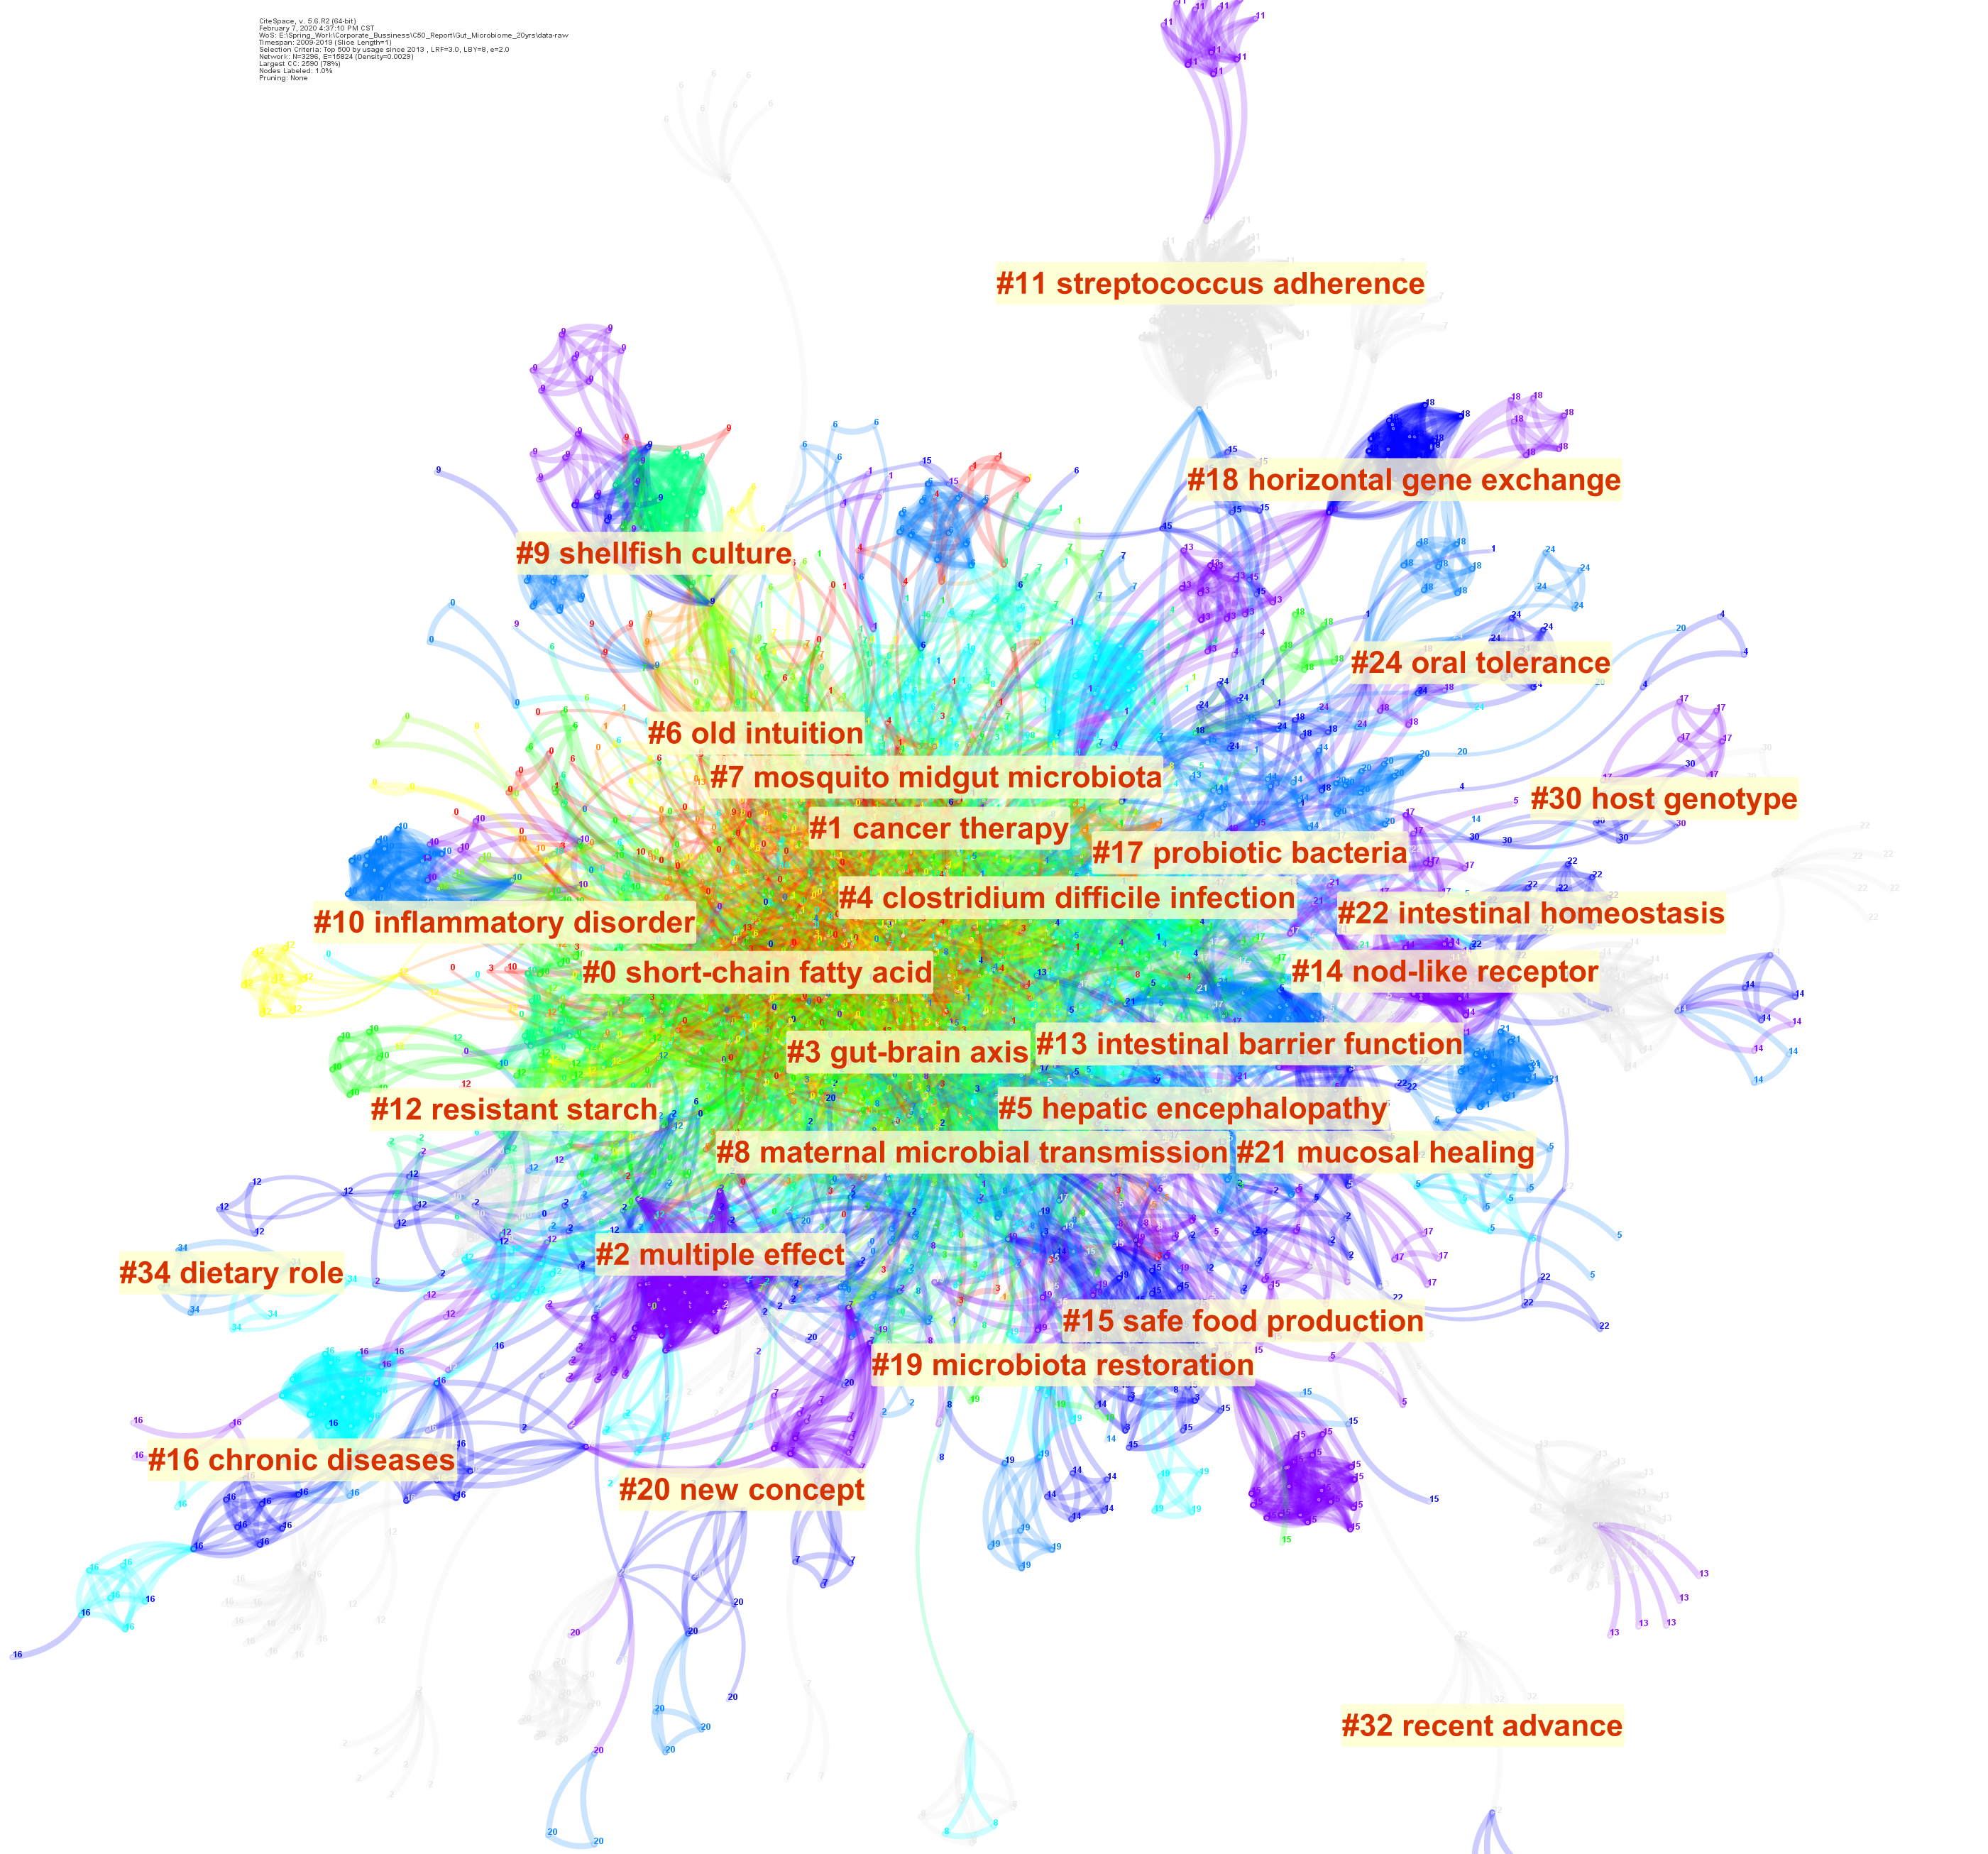
\includegraphics[width=1\linewidth]{citespace/citespace-highlycited-reference-network-complete} \caption{高被引论文的共被引网络(完整)}\label{fig:citespace-highlycited-reference-network-complete}
\end{figure}

\hypertarget{ux4f5cux8005ux7684ux5408ux4f5cux7f51ux7edc}{%
\subsection{作者的合作网络}\label{ux4f5cux8005ux7684ux5408ux4f5cux7f51ux7edc}}

我们接下来又分析了高被引论文的作者合作网络(图 \ref{fig:citespace-highlycited-author-network-complete})。

\begin{figure}
\includegraphics[width=1\linewidth]{citespace/citespace-highlycited-author-network-complete} \caption{高被引论文的作者合作网络(完整)}\label{fig:citespace-highlycited-author-network-complete}
\end{figure}

\hypertarget{ux5173ux952eux8bcdux7684ux5171ux73b0ux7f51ux7edc}{%
\subsection{关键词的共现网络}\label{ux5173ux952eux8bcdux7684ux5171ux73b0ux7f51ux7edc}}

关键词的共现网络,联系程度非常紧密,从中得到了 8 个研究主题,分别是:

\begin{enumerate}
\def\labelenumi{\arabic{enumi}.}
\tightlist
\item
  \#0 IBD
\item
  \#1 diet
\item
  \#2 metabolic syndrome(代谢综合征)
\item
  \#3 school age
\item
  \#4 gut-brain axis
\item
  \#5 gut microbiota
\item
  \#6 aquaculture/gastrointestinal microbiota
\item
  \#7 colorectal cancer(大肠癌)
\end{enumerate}

\begin{figure}
\includegraphics[width=1\linewidth]{citespace/citespace-highlycited-keyword-network} \caption{高被引论文的关键词共现网络}\label{fig:citespace-highlycited-keyword-network}
\end{figure}

\hypertarget{part-ux56fdux9645ux7814ux7a76ux683cux5c40}{%
\part{国际研究格局}\label{part-ux56fdux9645ux7814ux7a76ux683cux5c40}}

\hypertarget{global}{%
\chapter{全球合作网络}\label{global}}

在这一部分,我们将解析肠道菌群研究的国际合作关系。

\hypertarget{htmlwidget-a80db2d4b22126c54edd}{}

\label{fig:top-country-collaboration-sankey}主要国家间的合作关系

首先,我们看一下全球肠道菌群研究前 20 个国家间合作发表论文的情况。在图 \ref{fig:top-country-collaboration-sankey} 中,展示了两两之间合作发表论文的数量。例如,中美合作发表论文的数目有 1378 篇,这是所有国家中最多的;其次是英美之间合作发表论文的情形,有 898 篇;其次是美加之间合作发表论文 800 篇;再次是美德之间合作发表论文 705 篇;第五名是美法之间合作发表论文 522 篇。

这前五名中,都有\textbf{美国}的出现,说明了美国科学家在合作研究中占有的核心地位。

\hypertarget{htmlwidget-8ec7bf5b2dd24834f68c}{}

\label{fig:country-collaboration-network}国家间的合作网络

为了更直观的观察全球的合作网络,我们采用网络分析的方法进一步阐述。点的大小代表\emph{特征向量中心性},线的宽度表示国家间合作关系的多少(图 \ref{fig:country-collaboration-network})。这个网络是一个基本上完全连接的网络,即所有的 20 个国家与其它所有国家间都有合作关系的存在,为了简化这一网络,我们去掉了连接度小于100的边,得到上图。可以很明显的看出,与中国联系最紧密的国家依次是美国、英国、加拿大和澳大利亚。\emph{特征向量中心性}大的节点对相连的节点影响更大,因此可以直观的看到各个国家在整个合作网络中的重要性。

毫无疑问,美国是肠道菌群研究的领跑者。这不仅体现在美国的菌群研究开展的最早,体量最大,领域最广泛,而且体现在各大高校、研究所和社会力量的广泛参与上。除此之外,我们还可以发现当前肠道转化最积极的地方,也是美国。

\hypertarget{china-study}{%
\chapter{中国的肠道菌群研究}\label{china-study}}

在这一部分,我们将针对中国参与发表的研究论文进行文献计量学分析,以展示中国肠道菌群研究的全景。

\hypertarget{ux4e2dux56fdux7814ux7a76ux6982ux51b5}{%
\section{中国研究概况}\label{ux4e2dux56fdux7814ux7a76ux6982ux51b5}}

二十年间,中国发表论文的数量和比例双双增加(图 \ref{fig:china-publication-number})。

二十年前,我国基本没有相关的研究论文;十年前,即2010年,我国发表相关研究 82 篇,占当年全世界总发文量的 5\%;刚刚过去的2019年,我国发表相关研究论文超过 2500 篇,占当年全世界总发文量的 25\% 以上。自2013年以来,我国的论文发表量已经排到了世界第二的位置,仅次于美国。

从2009年开始,有我国科学家参与的高被引论文开始出现,高被引论文数量随之不断上升。最近三年(2017-1019),SCI高被引论文的数量都超过了35篇,成为能够贡献较多突出研究成果的国家之一。

\begin{figure}
\includegraphics[width=1\linewidth]{plots/china-publication-number-1} \caption{肠道菌群研究领域我国每年发表的SCI论文及其中的高被引论文的数量}\label{fig:china-publication-number}
\end{figure}

\hypertarget{ux7814ux7a76ux7684ux4e3bux8981ux8109ux7edc}{%
\subsection{研究的主要脉络}\label{ux7814ux7a76ux7684ux4e3bux8981ux8109ux7edc}}

我们使用历史引证网络分析的方法来厘清我国肠道菌群的研究脉络(图 \ref{fig:china-histnet})。历史引证网络中共包含了19篇关键文献,其主要信息列示在表 \ref{fig:china-histnet-articles} 中。接下来,我们将逐一回顾一下这些文献。

2008年发表在《美国科学院院刊(PNAS)》上的文章是一个重要的基点。该研究由上海交通大学赵立平教授、浙江大学第一附属人民医院李兰娟院士、中国国家人类基因组中心赵国屏院士和中国科学院武汉物理与数学研究所唐惠儒研究员实验室联合开展,并与伦敦帝国理工学院的JK Nicholson教授合作,第一作者是Li Min。研究的主要成果是发现了共生的肠道微生物调节人体的代谢表型。研究采用了代谢组学和宏基因组学相结合的方式,解析了7个中国人的粪便及尿液样本,并建立了菌群-宿主代谢连接的模型。研究在物种水平上发现了中国与美国人肠道菌群结构存在差异,并鉴定出最大影响宿主代谢和健康微生物组的关键功能成员的特征,如柔嫩梭菌群与尿液中8个代谢物有关,是菌群中功能性很强的成员,会影响许多宿主途径等。从代谢和宏基因组学的角度解释了人类与肠道菌群可以共同进化,并最终形成了密切的共生关系。

第二个关键研究是2010年发表在《Nature》杂志上的一篇论文,是中欧合作的人肠道宏基因组(MetaHIT)计划的最为关键成果之一。研究的主要负责人是中方华大基因的王俊和法方国立农学研究所的SD Ehrlich教授,研究的第一作者是华大基因的覃俊杰和李瑞强。该研究的主要成果是在人类肠道中鉴定出330万个微生物基因。人肠道菌群样本取自124个欧洲人的粪便标本。这些超过人类基因150倍的基因集包含了绝大多数人类的主要肠道微生物基因,并且大部分基因在人群中共有。细菌基因的比例超过99\%,这群人中共有约1100种的细菌,其中160个优势物种为人群所共有。

第三项关键研究2010年发表在《ISME J》杂志上,由赵立平教授和中科院上海生命研究所的Yan Chen领衔。该研究以小鼠建立实验动物模型,并借此揭示了肠道菌群、宿主基因和与饮食之间的相互作用在代谢综合征发展中的作用。

第四项关键研究2011年发表在《肝病学(Hepatology)》杂志上,由李兰娟院士和中科院北京微生物所的朱宝利研究员团队合作完成。该研究基于36名肝硬化患者和24名健康对照,得出了肝硬化相关的疾病菌群特征,并鉴定了与肝硬化相关的149个可操作性分类单元。

第五项关键研究2011年发表在《Nature》杂志上,也是MetaHIT的研究成果,主要是在人体中发现了三种肠型。华大基因参与了这一论文的发表。

第六项关键研究2012年发表在《Nature》杂志上,主要作者是华大基因的王俊、覃俊杰等人。本研究采用了微生物全基因组关联分析的方法(mGWAS)揭示了345个中国人的肠道菌群中存在的二型糖尿病标记物,并最终确定了23个肠道微生物标记物可以用于二型糖尿病的分类。

第七项关键研究2012年发表在《PLoS ONE》杂志上,主要作者是中科院武汉水生所的Guitang Wang。该项研究主要揭示了草鱼肠道菌群的典型特征,并推测影响草鱼肠道菌群的演化的三大因素分别是水体、底泥和饲料等。

第八项关键研究2012年发表在《ISME J》杂志上,仍然是由赵立平教授领衔。该项研究揭示了大肠癌患者中的疾病菌群特征,发现了11个与大肠癌高度相关的物种类群。

第九项关键研究是2013年发表在《Nature Reviews Microbiology》上面的一篇综述,由赵立平教授执笔,该研究探讨了如何揭示肠道菌群在肥胖中的作用,指出可以通过微生物组关联分析、宿主响应和无菌动物等手段来完成这一任务。

第十项关键研究2013年发表在《Nature》杂志上,揭示了与人体代谢性疾病相关的菌群特征{[}11{]}。华大基因参与了这一论文的发表。

第11项关键研究2013年发表在《ISME J》杂志上,通讯作者赵立平。在本研究中,在中国的肥胖人群中分离出一株产内毒素机会致病菌,可以促进无菌小鼠产生肥胖,从而建立了肠道菌群与肥胖之间的因果关系。

第12项关键研究2014年发表在《Nature》杂志上,通讯作者是李兰娟、郑树森(Shusen Zheng)和S. Dusko Ehrlich(伦敦国王学院)。该研究在第四项研究的基础上,进一步采用宏基因组技术和更大的人群分析了肝硬化相关的疾病菌群特征,得到了15个生物标记,可以用来准确的预测肝硬化。

第13项关键研究2014年发表在《Nature biotechnology》杂志上,主要作者是华大基因的团队。该研究公布了有史以来最大的肠道菌群参考基因组序列,包括近一千万个高质量的基因。

\hypertarget{htmlwidget-78143d5ff39869a5c571}{}

\label{fig:china-histnet-articles}我国肠道菌群研究的核心历史引证网络中列出的19篇研究论文的详细信息

第14项关键研究2015年发表在《Nature》杂志上,研究了二甲双胍这一二型糖尿病常用药对人肠道菌群的影响。华大基因参与了该项研究。

第15项关键研究2015年发表在《Nature Medicine》杂志上,主要研究了类风湿性关节炎患者口腔及肠道菌群受到扰乱且在治疗后部分恢复。主要参与单位是北京协和医学院和华大基因。

第16项关键研究2015年发表在《Nature Communications》杂志上,研究由台湾长庚大学的赖信志教授领衔,发现灵芝(水提取物)能通过调节肠道菌群的组成来降低小鼠肥胖。

第17项关键研究2015年发表在《Nature Communications》杂志上,研究由华大基因王俊领衔,揭示了结直肠腺瘤癌变过程中的肠道菌群特征。

第18项关键研究2015年发表在《ISME J》杂志上,由上海交通大学Jian Shen领衔。研究发现使用益生菌可以缓解高脂膳食小鼠具有的代谢综合征的症状。

第19项关键研究2018年发表在《Science》杂志上,由赵立平教授领衔。该研究成果利用膳食纤维改善了二型糖尿病的症状。

由我国的研究人员主导及参与的这19项关键研究,时间跨度从2008年到2018年,较完整的展示了我国肠道菌群研究的历史演替。即从认识肠道菌群的结构,到揭示菌群在肥胖、肝硬化等疾病中的作用,再到利用益生菌、益生元等干预措施来缓解和治疗一些肠道菌群相关的疾病。步步为营,稳扎稳打,奠定了我国肠道菌群研究的重要基石。

\hypertarget{ux4e3bux8981ux7684ux7814ux7a76ux673aux6784}{%
\section{主要的研究机构}\label{ux4e3bux8981ux7684ux7814ux7a76ux673aux6784}}

以论文发表量计算,20年间国内发表论文最多的研究机构分别是:中国科学院(中国科学院大学)、浙江大学、上海交通大学、中国农业大学和中国农业科学院等。

在前 30 名中,台湾的国立台湾大学、中国医药大学(台湾),以及香港的香港大学、香港中文大学等高校榜上有名,它们各自是相应地区的主要的肠道菌群相关研究机构。

\begin{figure}
\includegraphics[width=1\linewidth]{plots/china-top-university-1} \caption{参与我国肠道菌群研究的主要科研院所(展示发文量最多的30家)}\label{fig:china-top-university}
\end{figure}

在下方的研究机构合作网络中,大概可以看到 3 个主要的研究群体。

首先是以中科院为中心的主力研究团体,中科院作为一个核心,将各大高校和研究所有机的联系了起来;

其次是台湾地区的学术团体,除了前面提到的两所大学,还有国立阳明大学(NATL YANG MING UNIV)、台北医科大学(TAIPEI MED UNIV)、国立中兴大学(NATL CHUNG HSING UNIV)等,而宁波大学则是与之联系最紧密的大陆高校。

再次是以江南大学为核心的几所高校,包括北京工商大学(BTBU,BEIJING TECHNOL AND BUSINESS UNIV)、南京医科大学、南京大学等。

接下来是由北京中医药大学和中国中医学研究院组成的中医药方阵,以及第三军医大学和重庆医科大学组成的团体。

\hypertarget{htmlwidget-1f31fde0b74c864a3520}{}

\label{fig:china-aff-col-net}中国各大研究机构之间的合作关系

通过作者合作网络,可以更加清楚的看到国内各个研究团体,发现团队的带头人。

为了取得良好的可视化效果,我们对作者合作网络进行了简化,只保留了 200 个发文量最高的作者,同时删掉了合作发表论文数量小于 5 次的联系。这样,可以得到下面这幅图(图 \ref{fig:top-china-aut-col-net})。

\hypertarget{htmlwidget-c851239bc4cc8b62a35f}{}

\label{fig:top-china-aut-col-net}过去二十年间中国发表论文最多的200名作者之间和合作关系

如果不出意外的话,你将可以看到这里面最大的一个研究群体位于这幅图的中间。他又可以继续分成几个小团体。其中右边浅红色的部分,核心应当是李兰娟院士(LI, LANJUAN);绿色的部分,核心应当是赵立平教授(ZHAO, LIPING);深红色的部分,核心应当是贾伟教授(JIA, WEI);橙色的部分,核心应当是ZHU, WEIYUN。

与前面的一个群体不同,第二大的群体(上面橙色的部分)如果你放大来看,会发现这是一个联系非常紧密的团体,主要是华大基因及其合作者。其中包括了华大基因的汪俊(WANG, JUN),汪建(WANG, JIAN)等人。

在图片左下角的灰蓝色部分,我们可以找到陈卫院士(CHEN, WEI)的团队,这个铁四角包括赵建新(ZHAO, JIANXIN)、张灏(ZHANG, HAO)和王刚(WANG, GANG)等三位教授。

自此向右上方拖动,一个黄色的子网络是张和平教授(ZHANG, HEPING)的团队。右侧紧挨着的绿色子网络,是印遇龙院士(YIN, YULONG)的团队。

缩放网络,将焦点聚集在左上方的蓝色区域放大,可以观察到来自中国香港的研究群体。这一群体由于君教授(YU, JUN)、黄秀娟教授(NG,SIEW C)等人组成。

这幅网络中一共有数十个子网络,用不同的颜色标示。读者不妨找找,看有没有你认识的老师在这里面。

可以说,图中的这些人撑起了过去二十年中国肠道菌群研究的不同领域的天幕,让我们向他们致敬!

不同的研究群体可能有不同的高光时刻。为了证明这一假设,我们将2010-2019年的研究划分成3个阶段,分别观察合作网络的具体情况,比较网络中存在的差异。

可以发现,在第一个五年(2010-2014),是华大基因系集体出道的时刻,汪建等人组成了最大的一个合作团体(图 \ref{fig:top-china-aut-col-net-2010-2014} 中间绿色部分);其次,是李兰娟、周志刚、赵立平、贾伟、魏泓、李宁、钱大伟、陈卫等老师为核心的研究团队。这一批研究人员是较早开展肠道菌群相关研究的科学家。

\hypertarget{htmlwidget-e202d4b4feb684617220}{}

\label{fig:top-china-aut-col-net-2010-2014}2010-2014年间中国发表论文最多的100名作者之间和合作关系

接下来,在2015-2017这三年间,首先是汪建、赵立平、陈卫、李宁、魏泓、李兰娟等老师继续发光发热,同时也出现了印遇龙、张发明等新的有较多产出的研究力量(图\ref{fig:top-china-aut-col-net-2015-2017})。

\hypertarget{htmlwidget-10982a219c404cc59d17}{}

\label{fig:top-china-aut-col-net-2015-2017}2015-2017年间中国发表论文最多的100名作者之间和合作关系

在第三个阶段,即2017-2019年间,合作群体有了更加明显的改变。首先可以明显看到团体小型化的趋势比较明显,这可能意味着肠道菌群研究已经分化出较多差异比较明显的不同研究方向;其次,华大基因的研究群体,以及李兰娟、赵立平等人的团队开始变小;与此同时,王邦茂、朱永官、王军军、曹建新、周宏伟等新的研究群体开始成形。

\hypertarget{htmlwidget-8ffe182811e553df1b98}{}

\label{fig:top-china-aut-col-net-2018-2019}2018-2019年间中国发表论文最多的100名作者之间和合作关系

\hypertarget{ux7814ux7a76ux9886ux57df}{%
\section{研究领域}\label{ux7814ux7a76ux9886ux57df}}

肠道菌群的研究我们规划了八大领域,分别是饮食、免疫、代谢、癌症、心血管疾病、肠X轴、药物互作和中医药。可以发现前四大领域研究的发端较早,而后四大领域研究的发端则稍微晚一些。特别是``肠X轴''的研究,在2013年以后才逐渐壮大起来。

\begin{figure}
\includegraphics[width=1\linewidth]{plots/topic-nRecord-in-china-study-1} \caption{中国各研究主题关键论文数量对比}\label{fig:topic-nRecord-in-china-study}
\end{figure}

值得一提的是,这些研究领域之间相互之间是存在较多关联的。例如:代谢与饮食相关性最强,共享了777篇研究,代谢、免疫和饮食三者的重叠度也很高,共享了695篇研究论文。代谢、免疫、饮食这三个因素与癌症、心血管疾病两个肠道菌群相关的疾病之间的关联都十分紧密,体现了这些因素在疾病致病过程中的重要作用。与之相比,肠X轴和中医药研究作为较为独立、有中国特色的研究领域,再加上总体研究数目较少,所以它们与其它研究主题重叠度表现的并不高。除此之外,我们也可以看到免疫、代谢、饮食、癌症等四个领域下特有的研究数量也比较高,分别包括了712篇、605篇、477篇和187篇研究论文。

\begin{figure}
\includegraphics[width=1\linewidth]{plots/china-topic-upsetR-1} \caption{八大研究领域之间的重叠度。该图分为几个部分,左侧柱状图展示各研究领域的全部文章数目,右侧展示主题间文献的重叠度。其中右上方条形图展示相应研究领域重叠的文献数目。}\label{fig:china-topic-upsetR}
\end{figure}

\hypertarget{ux53d1ux5c55ux8d8bux52bf}{%
\section{发展趋势}\label{ux53d1ux5c55ux8d8bux52bf}}

为了揭示我国肠道菌群研究的发展趋势,我们将近十年最热的关键词做一个梳理。因为早期研究论文数量比较少,所以我们将这十年分成了5年,3年和2年的三个阶段,并进一步结合文章关键字的共现网络来进行阐述。

第一个阶段(图 \ref{fig:keyword-net-2010-2014}),自2010年到2014年,关键字的共现网络一共只有9个关键词,其中最突出的是饮食诱导的肥胖(Diet-induced obesity)、炎症(inflammation)和胰岛素抗性(insulin resistance)。这直观的反映了我们对肠道菌群的认知是始于对肥胖机制的新认识。这一新认识或许可以由肥胖(Obesity)和多样性(Diversity)之间的关系来指代------这是另外两个与肥胖相关的核心关键词。除此之外,还可以发现16S rRNA与人粪便有了重要的联系,直观来看,这意味着16S rRNA基因测序技术的进步在肠道菌群研究中起到了关键的推动作用。但可能会被忽视的一点是,选择粪便样本作为研究对象在这其中也功不可没。这五年间的另两个关键词是溃疡性结肠炎和克罗恩病,它们与肠道菌群失衡的关系逐步被揭示。

\hypertarget{htmlwidget-bfc0412ee330fc39f701}{}

\label{fig:keyword-net-2010-2014} 2010年-2014年间的研究热点。图中的点表示研究论文的关键词,线表示关键词的共现关系(即两个关键词同时出现在一篇文献中)。点的大小指示对应关键词出现次数的多少,线的粗细指示关键词共现关系的强弱。为简化图形,共现次数少于3次的在图中不可见。同时,孤立的关键词也被删除。

第二个阶段(图 \ref{fig:keyword-net-2015-2017}),自2015年到2017年,三年间的关键字共现网络比第一个阶段已经明显更加丰富。肥胖、炎症、饮食、多样性等关键字蝉联入榜。除此之外,健康、疾病、代谢和小鼠等相关研究也成为主要的研究主题。特别值得关注的是小鼠-炎症之间具有特别强的共现关系,这体现了小鼠作为模式动物在相关研究中已经处于不可或缺的地位。此外,多样性-代谢之间也具有特别强的共现关系,说明在多样性之上,研究人员开始关注菌群的代谢产物------而代谢产物被后来证明是重要的菌群效应分子。图中也可以发现,胆碱(Phosphatidylcholine)是这一阶段重点关注的代谢物。这一时期,肠道菌群与肿瘤之间的关系被进一步理解,在图中这体现在具核梭杆菌(Fusobacterium nucleatum)与肿瘤之间的较强的共现关系上。除此之外,蔗糖和减脂手术(Bariatric surgery)之间的关系也在这一阶段的研究中处于比较突出的地位。

\hypertarget{htmlwidget-711cc3b1207186563016}{}

\label{fig:keyword-net-2015-2017}2015-2017年间主要的研究方向(WoS关键词)

第三个阶段,2018年到2019年,这两年间的研究主题呈现出异彩纷呈的情形。首先,我们可以发现炎症的关键地位得到加强,甚至已经处于核心节点的位置上,所有其它的研究主题都直接或者间接的与其相连。而炎症之外,在肥胖、胰岛素抗性、代谢、健康等传统主题的基础上,大量增加了毒性(toxicity)、激活(activation)、暴露(exposure)、调节(modulation)等与环境因子相关的研究主题,特别是阿特拉津(atrazine)和多酚类(polyphenols)这两种典型环境污染物的出现,标志着环境微生物学与肠道菌群的结合成为主流。还可以看到,(短)链脂肪酸(chain fatty acids)作为一个关键的菌群代谢产物,在这一时期成为主要研究主题。一些机制相关的主题词也开始出现,如基因表达,蛋白偶联受体等,标志着肠道菌群的作用机制逐渐明确。特别值得一提的是,大脑出现在这一阶段的关键词中,这反映了肠脑轴相关研究在此期间取得的进步。

\hypertarget{htmlwidget-9a7d290be55d937f9fda}{}

\label{fig:keyword-net-2018-2019}2018-2019年间主要的研究方向(WoS关键词)

\hypertarget{ux589eux957fux6700ux4e3aux8fc5ux901fux7684ux5173ux952eux5b57ux6709ux54eaux4e9b}{%
\subsection{增长最为迅速的关键字有哪些?}\label{ux589eux957fux6700ux4e3aux8fc5ux901fux7684ux5173ux952eux5b57ux6709ux54eaux4e9b}}

从图 \ref{fig:china-study-keyword-growth} 可以看到,Activation、细菌、(短)链脂肪酸,饮食、疾病、多样性、表达、健康、感染、炎症等关键词是近十年增长最快的关键词。

\begin{figure}
\includegraphics[width=1\linewidth]{plots/china-study-keyword-growth-1} \caption{2010-2019年增长最快的30个研究关键词}\label{fig:china-study-keyword-growth}
\end{figure}

\hypertarget{ux6e2fux6fb3ux53f0ux5730ux533aux7684ux80a0ux9053ux83ccux7fa4ux7814ux7a76}{%
\section{港澳台地区的肠道菌群研究}\label{ux6e2fux6fb3ux53f0ux5730ux533aux7684ux80a0ux9053ux83ccux7fa4ux7814ux7a76}}

与大陆相比,港台地区的肠道菌群研究开始的可能还要更早一些,在2005年以前,研究数量普遍较少,而港台地区的发文量可以占到全国的四分之一以上。
进入2010年以后,由于大陆相关研究的强势崛起,港台地区的论文比例稳步下降。到了2019年,大陆已经成为绝对的中流砥柱。

通过图 \ref{fig:mainland-hongkong-macao-taiwan} 也可以发现,总体上大陆和港台地区的相关研究是同一时期起步的,而澳门可能稍显迟疑。

\begin{figure}
\includegraphics[width=1\linewidth]{plots/mainland-hongkong-macao-taiwan-1} \caption{中国大陆和港澳台地区的研究概况}\label{fig:mainland-hongkong-macao-taiwan}
\end{figure}

那么,究竟港澳台地区有哪些研究机构参与其中?又与大陆哪些科研院所有比较多的交流合作呢?请看下面的分析结果。

首先看台湾省主要的研究机构,包括岛内的多所大学(特别是医学院校)、中研院和荣军医院等,岛外的合作单位可见美国罗格斯州立大学,而与大陆的研究机构之间的合作较少。

\hypertarget{htmlwidget-7f04e5565dad629984fc}{}

主要的研究立足点与中国总体结构还是比较类似的,像炎症、疾病、健康、饮食、肥胖等关键词都有出现且均占主要地位。

\hypertarget{htmlwidget-a91464da40b7393b5e9e}{}

与台湾相比,香港的研究机构与域外机构间的合作则十分常见。在下方的研究机构合作网络中,内地、欧洲的多所科研院所均名列其中。从中也可以发现,香港大学是香港肠道菌群研究的生力军。

\hypertarget{htmlwidget-3f369558586d1f29ef92}{}

从香港肠道菌群研究的关键词共现网络中,可发现他们对溃疡性结肠炎、克罗恩病这两种疾病的研究较多。

\hypertarget{htmlwidget-2bcd30b20e1d795d9704}{}

澳门的肠道菌群研究体量最小,其研究领域也最少,在此不再详述。

\hypertarget{htmlwidget-93e1c4870ab0a3a586e4}{}

\hypertarget{htmlwidget-2c1327a2a505093dbd9d}{}

\hypertarget{part-ux7814ux7a76ux70edux70b9}{%
\part{研究热点}\label{part-ux7814ux7a76ux70edux70b9}}

\hypertarget{research-topic}{%
\chapter{四大研究主题}\label{research-topic}}

我们都知道,对于肠道菌群研究而言,饮食、免疫、代谢、疾病等是四大最重要的研究主题。在这一部分,我们将在这四大研究主题之间逐步展开。

\hypertarget{ux4e3bux9898ux5bf9ux5e94ux7684ux6838ux5fc3ux8bbaux6587ux6570ux636e}{%
\section{主题对应的核心论文数据}\label{ux4e3bux9898ux5bf9ux5e94ux7684ux6838ux5fc3ux8bbaux6587ux6570ux636e}}

我们首先统计下各个研究主题相关的论文数量。

在接下来的分析中,我们将基于 3345 篇\textbf{关键论文}进行。显而易见,每个研究主题都具有庞大的发文量(图 \ref{fig:topic-nRecord-in-core-articles})。

\begin{figure}
\includegraphics[width=1\linewidth]{plots/topic-nRecord-in-core-articles-1} \caption{各研究主题关键论文数量对比}\label{fig:topic-nRecord-in-core-articles}
\end{figure}

与此同时,也可以看到这四大研究主题都是历史比较悠久的研究领域(图 \ref{fig:topic-trend-in-core-articles}),自 2000 年以来不断有关键的研究论文发表。

\begin{figure}
\includegraphics[width=1\linewidth]{plots/topic-trend-in-core-articles-1} \caption{各研究主题发表的关键论文数量变化情况}\label{fig:topic-trend-in-core-articles}
\end{figure}

四大研究主题间的重叠度也相当可观(图 \ref{fig:overlap-of-topic-in-core-article})。 其中,免疫和疾病的文献重叠度最高,免疫、代谢和疾病的重叠度次之,而四大研究主题共有的研究论文就有 511 篇,占到全部\textbf{关键论文}的近六分之一之多\ldots\ldots{}

\begin{figure}
\includegraphics[width=1\linewidth]{plots/overlap-of-topic-in-core-article-1} \caption{各研究主题核心论文间的重叠度}\label{fig:overlap-of-topic-in-core-article}
\end{figure}

\hypertarget{diet}{%
\chapter{肠道菌群与饮食}\label{diet}}

\hypertarget{ux6838ux5fc3ux6587ux7ae0ux5217ux8868}{%
\section{核心文章列表}\label{ux6838ux5fc3ux6587ux7ae0ux5217ux8868}}

\hypertarget{htmlwidget-c921cb4092fa53d28b17}{}

\label{fig:diet-article-datatable}饮食相关研究的核心论文

首先奉上``饮食''相关研究的关键论文清单,如果有《热心肠日报》解读的话,也一并附上(图 \ref{fig:diet-article-datatable})。
这里包括了 1352 篇论文,包括 497 篇高水平综述,其中有中文短科普的就有 421 篇。
如果你是一个初学者,可按此图索骥,快速把握肠道菌群与饮食相关的研究内容。

\hypertarget{ux9886ux57dfux5185ux4e13ux5bb6}{%
\section{领域内专家}\label{ux9886ux57dfux5185ux4e13ux5bb6}}

图 \ref{fig:diet-article-top-author} 中列出了本领域知名专家,其中就包括我们前面(\ref{top-scientist})介绍过的两位最出众的科学家:
KNIGHT, ROB 和 GORDON, JEFFERY I.。应该说,后者在饮食研究领域的贡献更为突出,因为你将会看到历史脉络中的绝大多数文章都是由他们课题组完成的。

\begin{figure}
\includegraphics[width=1\linewidth]{plots/diet-article-top-author-1} \caption{饮食相关研究的顶尖学者}\label{fig:diet-article-top-author}
\end{figure}

从作者合作网络中(图 \ref{fig:diet-article-author-collaboration-network}),可以发现 Rob Knight 和 Jeffrey I. Gordon 是来自于同一个研究群体,这一群体还有 3 个重要人物,分别是 Bernard Henrissat,Dan Knights 和 Federico E. Rey。

除此之外,我们还可以发现 5 个其他的研究群体。

\begin{itemize}
\item
  Hazen, Stanley L., Wang, Zeneng, Tang, W. H. Wilson, Wu, Yuping 和 Lusis, Aldons J.
\item
  Cryan, John F., Dinan, Timothy G. 等人
\item
  Cani, Partrice D., Delzenne, Nathalie M. 等人
\item
  Flint, Harry J., Duncan, Sylvia H. 等人
\item
  Ventura, Marco 等人
\end{itemize}

\hypertarget{htmlwidget-8d05998c4e2890c11196}{}

\label{fig:diet-article-author-collaboration-network}饮食相关研究的主要作者合作网络。显示发文量最多的 30 位研究者之间的合作关系。

\hypertarget{ux673aux6784ux5408ux4f5cux7f51ux7edc}{%
\section{机构合作网络}\label{ux673aux6784ux5408ux4f5cux7f51ux7edc}}

从发文量看机构排行,前30家机构中领衔的圣路易斯华盛顿大学(WASHINGTON UNIV)、哥本哈根大学(UNIV COPENHAGEN)和科罗拉多大学(UNIV COLORADO)等(图 \ref{fig:diet-univeristy-top30})。

\begin{figure}
\includegraphics[width=1\linewidth]{plots/diet-univeristy-top30-1} \caption{饮食相关研究发文量最高的30家机构}\label{fig:diet-univeristy-top30}
\end{figure}

观察机构间的合作网络,可以发现科罗拉多大学和天主教鲁汶大学(CATHOLIC UNIV LOUVAIN)处于网络中非常核心的地(图 \ref{fig:diet-article-university-collaboration-network})。哥本哈根大学与哥德堡大学(UNIV GOTHENBURG)之间的合作强度比较大。

\hypertarget{htmlwidget-798f4f84e2f066126930}{}

\label{fig:diet-article-university-collaboration-network}饮食相关研究机构合作网络
这个网络中的节点取自本领域发文量最大的30家机构,机构间的连线表明二者存在合作发表论文的情况。连线的线越粗,说明二者间的论文发表数量越多。点的大小越大,说明其在合作网络中处于更重要的节点位置。为了更好的显示效果,本图经过适当简化,去掉了孤立的点和较弱的连接。

\hypertarget{ux7814ux7a76ux70edux70b9}{%
\section{研究热点}\label{ux7814ux7a76ux70edux70b9}}

从这些研究使用的关键词,可以瞥见研究的热点。最受关注的30个关键词中,最值得关注的是(短)链脂肪酸(Chain Fatty-acids),
这一个关键词的文章数量仅次于肠道菌群的两种不同表达方法(Gut microbiota 和 intestinal microbiota),排在了多样性(Diversity)的前面。

而肥胖(Obesity)作为与饮食关系最为密切的一种常见病,排在了第6位。其它一些疾病相关的关键词,包括炎症、IBD(Inflammatory-bowel-disease)、
胰岛素抗性(Insulin resistance)、IBS(Irritable bowel syndrome)、克罗恩病(Crohns Disease)等
(图 \ref{fig:diet-id-top30})。

\begin{figure}
\includegraphics[width=1\linewidth]{plots/diet-id-top30-1} \caption{以文章数量计,最受关注的关键词(Top30)}\label{fig:diet-id-top30}
\end{figure}

这些关键词组成了如下所示的一个共现网络(图 \ref{fig:diet-id-top30})。
不出意外,肥胖和(短)链脂肪酸在网络中占据最突出的地位。
可以发现,蛋白偶联受体(Protein Coupled Receptor)和(短)链脂肪酸之间有着非常强的联系,
意味着前者在后者的功能中具有重要的作用。

\hypertarget{htmlwidget-d8bf19b04221ff07d99b}{}

\label{fig:diet-id-network}关键词共现网络包括了相关研究中最长出现的50个关键词。
为突出网络主体,一些孤立的节点和较弱的连接被隐去。

\hypertarget{ux80a0ux9053ux83ccux7fa4ux4e0eux996eux98dfux7814ux7a76ux7684ux5386ux53f2ux8109ux7edc}{%
\section{肠道菌群与饮食研究的历史脉络}\label{ux80a0ux9053ux83ccux7fa4ux4e0eux996eux98dfux7814ux7a76ux7684ux5386ux53f2ux8109ux7edc}}

接下来,我们通过观察这些文章的\textbf{历史引证网络},来理清相关研究的脉络(图 \ref{fig:diet-article-histnet})。

\begin{figure}
\includegraphics[width=1\linewidth]{plots/diet-article-histnet-1} \caption{饮食相关文献的核心引证网络}\label{fig:diet-article-histnet}
\end{figure}

\hypertarget{ux83ccux7fa4ux88abux53d1ux73b0ux662fux996eux98dfux4e0eux80a5ux80d6ux4e4bux95f4ux91cdux8981ux7684ux4e00ux73af}{%
\subsection{菌群被发现是饮食与肥胖之间重要的一环}\label{ux83ccux7fa4ux88abux53d1ux73b0ux662fux996eux98dfux4e0eux80a5ux80d6ux4e4bux95f4ux91cdux8981ux7684ux4e00ux73af}}

从图 \ref{fig:diet-article-histnet} 中可以看到,最早的一篇研究可以追溯到 2004 年\citep{backhedGutMicrobiotaEnvironmental2004}。
这篇发表在 PNAS 上的研究论文使用无菌小鼠做了饲喂实验,结果发现正常小鼠体内的肠道菌群能够促进无菌小鼠对糖类的吸收,并促进脂肪的累积。
而如果没有肠道菌群的作用,无菌小鼠中的脂肪累积就会显著下降。不仅如此,该研究还鉴定出小鼠中的 Fiaf 基因在微生物参与的脂肪累积中发挥重要作用,从而说明了肠道菌群是一个影响饮食能量吸收和储存的重要因素。

同样是 Bäckhed F,同样是在 PNAS 上面,2007 年他们又发表了一篇研究论文,阐明了无菌小鼠之所以不会肥胖的分子机制\citep{backhedMechanismsUnderlyingResistance2007}。
这项研究针对前一项研究中一个有意思的现象展开,那就是无菌小鼠在面对高脂、高糖的西式饮食时,较有菌小鼠更加不容易出现脂肪累积。
原因是什么呢?一种途径可能在于肠道细胞中通常被抑制的 Fiaf 基因的上调,另一种途径在于骨骼肌和肝脏中磷酸化的AMPK水平的上升。
由于菌群是 Fiaf 基因表达的一个抑制因素,所以当菌群不存在时,Fiaf 基因就会上调,导致下游脂肪酸代谢基因的失调,不利于脂肪累积。
而AMPK下游相关的脂肪酸代谢基因同样也是如此。所以,两种相互独立的信号通路参与了饮食因素在小鼠肥胖中的作用,而根源都与肠道菌群息息相关。

同年发表的另一篇文章,将肠道菌群之所以能够促进肥胖的关键诱发因素给鉴定了出来,那就是细菌分泌的内毒素,具体而言是细菌的脂多糖(LPS)\citep{caniMetabolicEndotoxemiaInitiates2007}。
CANI PD 等的研究发现,细菌脂多糖能够进入人体血液并作用于 CD14 细胞,从而引起代谢性的炎症,最终导致全身性的胰岛素抵抗,提高小鼠肥胖和糖尿病风险。
而不管是降低 LPS 浓度还是突变 CD14,都能够抑制小鼠糖尿病和肥胖症的发作。

\hypertarget{ux4e0dux8bbaux662fux957fux671fux8fd8ux662fux77edux671fux996eux98dfux90fdux662fux80a0ux9053ux83ccux7fa4ux6700ux91cdux8981ux7684ux5f71ux54cdux56e0ux7d20ux4e4bux4e00}{%
\subsubsection{不论是长期还是短期,饮食都是肠道菌群最重要的影响因素之一}\label{ux4e0dux8bbaux662fux957fux671fux8fd8ux662fux77edux671fux996eux98dfux90fdux662fux80a0ux9053ux83ccux7fa4ux6700ux91cdux8981ux7684ux5f71ux54cdux56e0ux7d20ux4e4bux4e00}}

在另一篇论文中,研究人员分析了饮食饮食在婴儿肠道菌群发育中可能的作用\citep{palmerDevelopmentHumanInfant2007}。
这项研究一共纳入了 14 个健康的婴儿,包括一对同卵双胞胎。因为早期研究方法的局限性,作者用了非常多的方法来跟踪婴儿肠道菌群随时间的变化过程,
其中包括基因芯片、qPCR、16S rRNA基因克隆和测序等。最终分析了 548 个样本,包括婴儿的粪便、母亲的阴道拭子和粪便、父亲和兄弟姐妹的粪便,以及母乳等等。
并初步分析了疾病、药物、饮食变化和旅行等关键事件对菌群的影响。

TURNBAUGH PJ 2009年的另一个研究,选取成年女性同卵及异卵双胞胎(同一对双胞胎胖瘦一致),分析其与其母亲的粪便菌群,研究宿主基因型、环境暴露及宿主肥胖如何影响肠道菌群\citep{turnbaughCoreGutMicrobiome2009}。一共分析了154个个体,结果显示家庭成员之间既共享部分肠道菌群,也存在群落组成的差异,差异程度在同卵双胞胎与异卵双胞胎中相似。同时发现,在基因水平而菌群谱系水平,所有个体拥有一个核心菌群。

\begin{figure}
\includegraphics[width=1\linewidth]{images/filippoImpactDietShaping2010_fig1} \caption{非洲乡村的风貌和居民饮食[@filippoImpactDietShaping2010]}\label{fig:filippoImpactDietShaping2010-fig1}
\end{figure}

2010年DE FLILIPPO 发表在 PNAS 上的那篇论文,通过比较欧洲和非洲农村地区儿童的肠道菌群和饮食差异,发现饮食是塑造肠道菌群的关键因素\citep{filippoImpactDietShaping2010}。在非洲农村(图 \ref{fig:filippoImpactDietShaping2010-fig1}),儿童饮食中含有更多的植物多糖,相应地造成肠道菌群中有更加丰富的拟杆菌门细菌,更加少的厚壁菌门细菌,以及非常丰富的普雷沃氏菌和 \emph{Xylanibacter}。后者被认为在纤维素和木聚糖的水解中发挥重要作用,在欧洲儿童肠道菌群中没有发现。

WALKER AW 2011年的论文研究了10周的时间跨度内,不同类型饮食对志愿者肠道菌群的调节作用\citep{walkerDominantDietresponsiveGroups2011}。研究除了对照组,还有高抗性淀粉饮食、非淀粉多糖饮食和低糖饮食等3种。2名志愿者的结果显示抗性淀粉饮食中 60\% 的抗性淀粉仍然没有被消耗,这使得肠道菌群产生了明显的变化,包括瘤胃球菌和 \emph{Oscillibacter} 等厚壁菌门细菌的显著增加。
这表明食物中不可被人类利用的成分会对肠道菌群的结构产生显著影响。

沿着这条线走下去,是 TURNBAUGH PJ 在2008/2009年发表的三篇重要研究。在 2008 年发表的 Cell Host and Microbe 杂志的研究中报道了肥胖与小鼠远端肠道菌群改变相关\citep{turnbaughDietInducedObesityLinked2008},主要表现在两个方面:一是发现西式饮食能够促进厚壁菌门柔膜菌纲的激增,而限制饮食控制肥胖后这种现象消失;二是发现将这个胖鼠的菌群移植到瘦的无菌小鼠中后,会大大促进瘦鼠脂肪的堆积。

在 2009 年发表在 Science Translational Medicine 杂志上的研究,则通过将人的肠道菌群移植到无菌小鼠中,研究``人鼠合一''的肠道菌群如何被饮食调控\citep{turnbaughEffectDietHuman2009}。
结果发现,首先人的肠道菌群是可以在小鼠内定殖的,且定殖后的菌群特征与人类的相似。其次,当从低脂、富含膳食纤维的饮食转向高脂高糖的西式饮食后,
可在一天内改变肠道菌群的结构,以及菌群的代谢、基因表达等。本研究同时也发现,与定殖的历史相比,饮食是改变菌群更重要的因素。

而在 2011 年,PNAS 上的另一项研究通过观察婴儿肠道菌群的演替,最终明确婴儿微生物组的改变与生活事件(包括饮食、健康状态等)是密切相关的\citep{koenigSuccessionMicrobialConsortia2011}。
辅食的添加是促进婴儿肠道菌群转向成人的重要因素。

进一步地,在成人中也观测到饮食对肠道菌群的显著调节作用\citep{wuLinkingLongtermDietary2011}。食用\textbf{高脂/低膳食纤维}或者\textbf{低脂/高膳食纤维}的饮食,24小时内就可以改变肠道菌群。前者引起拟杆菌的上升,后者引起普雷沃氏菌的上升。鉴于这两种菌是肠型的主要定义类群,因此长期的饮食作用下,会改变一个人的肠型。这一现象不仅出现在人身上,其它哺乳动物中也是如此\citep{mueggeDietDrivesConvergence2011}。紧接着,在2014年,DAVID LA 在 Nature 杂志发文阐释了\textbf{动物来源食物}和\textbf{植物来源食物}短期内对肠道菌群的影响\citep{davidDietRapidlyReproducibly2014},他们同时发现,动物来源的食物通过\emph{Bilophila wadsworthia} 与炎症性肠病关联了起来。

2012 年发表在 Nature 的两篇论文关注了更多人群中肠道菌群与饮食和健康之间的关系\citep[\citet{yatsunenkoHumanGutMicrobiome2012}]{claessonGutMicrobiotaComposition2012}。通过比较婴儿、儿童和成人的肠道菌群差异,明确了肠道菌群随年龄的变化趋势\citep{yatsunenkoHumanGutMicrobiome2012}。此外,也发现美国与其它国家居民的肠道菌群存在差异\citep{yatsunenkoHumanGutMicrobiome2012}。虽然地域也是菌群差异的重要因素,但是最直接的原因仍然被锚定在了饮食上。例如:与地理位置相比,饮食是老年人肠道菌群差异的主要决定因素\citep{claessonGutMicrobiotaComposition2012}。

\hypertarget{ux996eux98dfux6f14ux53d8ux4e3aux4e00ux79cdux91cdux8981ux7684ux5e72ux9884ux624bux6bb5}{%
\subsubsection{饮食演变为一种重要的干预手段}\label{ux996eux98dfux6f14ux53d8ux4e3aux4e00ux79cdux91cdux8981ux7684ux5e72ux9884ux624bux6bb5}}

SOKOL H 2008年发表在 PNAS 上的研究,主要是鉴定了克罗恩病患者肠道内一种抗炎共生细菌 \emph{Faecalibacterium Prausnitzii}\citep{sokolFaecalibacteriumPrausnitziiAntiinflammatory2008}。
\emph{F. Prausnitzii}是厚壁菌门的一员,在CD复发患者中的比例显著降低。而该菌存在时,其分泌的代谢产物能够抑制肠道细胞的炎症反应。
这一研究虽然并不直接与饮食相关,却是饮食干预治疗 CD 的重要基础。

饮食对肠道菌群结构性的改变只是表象,与之相比,更重要的是肠道菌群对食物中不同营养成分代谢能力的差异。这不仅影响人的消化能力,还会改变一些疾病的患病风险。2011年 WANG ZN 发表在 Nature 杂志上的论文,就发现菌群的代谢产物氧化三甲胺(TMAO)是心血管疾病重要的风险因素\citep{wangGutFloraMetabolism2011}。TMAO由肠道菌群代谢胆碱后生成,吸收进入血液后可以促进动脉粥样硬化。在易患动脉粥样硬化的小鼠中抑制肠道菌群,可抑制饮食中胆碱增多带来的动脉粥样硬化。

随后,在2013年 Nature Medicine 上,KOETH RA 发表论文表示红肉中的肉碱是肠道菌群代谢产生 TMAO 的可用来源之一\citep{koethIntestinalMicrobiotaMetabolism2013},从而解开了红肉与动脉粥样硬化之间的内在关联。

RIDAURA VK 2013年发表在 Science 上面的论文,用人粪菌移植的方法,描述了通过调节菌群改善肥胖的可能性\citep{ridauraGutMicrobiotaTwins2013a}:\href{https://www.mr-gut.cn/papers/read/1050193804}{移植胖人粪菌的小鼠,长得更胖}。

自此,饮食开始成为一种重要的干预手段,被广泛应用于疾病治疗、健康保健中。

\hypertarget{ux517bux51faux597dux83ccux7fa4}{%
\subsection{养出好菌群}\label{ux517bux51faux597dux83ccux7fa4}}

历史研究脉络展示了2014年前的20篇关键论文,而饮食与肠道菌群的故事当然还在继续。
通过前面的这些研究,我们意识到肠道菌群具有人类没有的代谢能力,主要是大多数的植物多糖都不会被人类消化,所以会进入结肠成为肠道菌群的潜在食物来源。
细菌不同菌株具有分解不同底物的多样性和诱导能力,整个菌群具有数千个参与碳水化合物分解代谢的基因\citep{farrellImportanceFeedingYour2019}。

值得注意的是,肠道菌群中的一些成员,不仅可以利用食物中的聚糖成分,在膳食纤维不足的情况下,还会去分解肠道内的粘膜聚糖,从而导致结肠粘膜屏障的侵蚀。
所以养出好菌群非常重要!你得给它吃菜,如果没有菜它只能去啃你的肠子\citep{desaiDietaryFiberDeprivedGut2016}。
这可能是饮食诱发肠道菌群失调后引起肥胖、炎症性肠病等肠道疾病的重要途径之一。

反过来,如果我们能够弄清楚不同的肠道菌群成员对营养的不同偏好,那么调节肠道菌群将变成一种操作性很强的工作。
例如,2018 年 Nature 上面发表的一篇论文,
使用 \href{https://www.mr-gut.cn/papers/read/1065476652}{改造菌株+配套营养支持=可精细调控的菌株定殖}。
他们向拟杆菌株中转化可利用紫菜聚糖的罕见基因位点,使之能利用紫菜聚糖作为碳源;
通过喂食紫菜聚糖,在小鼠肠道中形成一种独有的代谢生态位,以供这种改造的外源菌株独享,使该菌株可以在含有不同肠道菌群的小鼠中成功植入;
调节紫菜聚糖的喂食剂量,可精细调控该菌株在小鼠肠道内的丰度,且该效果可逆;
这种靶向的膳食营养支持,足以使改造的外源菌株与已在小鼠结肠隐窝内定殖的同基因型菌株竞争,并取代后者。

未来,如果我们弄清楚了菌群中不同组分在健康或者疾病中的作用,那么靶向菌群的``精准营养''或许可以成为一种非常有效的治疗手段。

\hypertarget{immunity}{%
\chapter{肠道菌群与免疫}\label{immunity}}

在这个章节,我们主要讨论肠道菌群与免疫的相关研究。

西方一位著名的哲学家尼采曾经说过:那些杀不死你的,终将使你更加强大。
如果用这句话用来形容肠道微生物与免疫的关系,真是再合适不过了。

作为人体内最大的微生物群落的栖息地,肠道中的菌群数量与人身上人类细胞的数目几乎相当。
这股不可忽视的力量与肠道粘膜间的相互作用因此成为人体免疫前线最重要的部分。

\hypertarget{ux514dux75abux76f8ux5173ux7684ux6838ux5fc3ux6587ux7ae0ux5217ux8868}{%
\section{免疫相关的核心文章列表}\label{ux514dux75abux76f8ux5173ux7684ux6838ux5fc3ux6587ux7ae0ux5217ux8868}}

\hypertarget{htmlwidget-452485524d5a51c925ea}{}

\label{fig:immune-article-datatable}免疫相关的核心文章列表

在图 \ref{fig:immune-article-datatable} 中,列出了 20 年来肠道菌群与免疫相关研究的核心论文,
一共有 2088 篇。近几年的新文献,过半有相应的《热心肠日报》解读。
通过阅读短科普,可以帮助你快速熟悉这一研究领域。

\hypertarget{ux7814ux7a76ux529bux91cf}{%
\section{研究力量}\label{ux7814ux7a76ux529bux91cf}}

首先,我们看一下全球尺度上,相关研究的科学家、团体都有哪些。

在图 \ref{fig:immune-article-top-author} 中,列出了发文量最高的十位科学家,
以及他们每年发表的文章数量和被引用的次数。
由图可知,Xavier, Ramnik J. 是相关研究成果最突出的科学家,他最近几年的产出也非常稳定,
主要研究领域是炎症性肠病(IBD)。炎症性肠病,顾名思义,就是肠道的炎症所引起的疾病。
它目前是一种原因不明的疾病,也缺乏有效的治疗手段。
但是已知是由异常的免疫所介导的肠道炎症,这种炎症它反复发作,甚至可以伴随患者终生。
Xavier, Ramnik J. 的研究成果包括鉴定 IBD 相关的菌群特征、遗传位点和免疫途径等等。

第二名 Knight, Rob 是一个计算生物学家,他发展了现在最流行的宏基因组分析流程,
同时也是肠道菌群研究最为知名的科学家之一。不过,他的主要研究成果可能不仅仅限于免疫这一话题,
在此不多做介绍。

第三名,Cryan, John F. 则是研究``肠脑轴''领域的知名科学家之一。
一些神经性疾病,包括抑郁症、焦虑等都与肠道菌群免疫、代谢等存在关联,
Cryan, John F. 的研究就在于揭示``肠脑轴''相关的作用机制,寻求新的治疗手段等。

\begin{figure}
\includegraphics[width=1\linewidth]{plots/immune-article-top-author-1} \caption{肠道菌群与免疫领域内顶尖专家}\label{fig:immune-article-top-author}
\end{figure}

第四名,Huttenhower, Curtis ,他与 Xavier 是合作关系比较紧密的一名研究者,
可能来自于同一团队(图 \ref{fig:immune-article-author-collaboration-network})。

第五名,Dinan, Timothy G. 则是 Cryan 最主要的合作者之一(图 \ref{fig:immune-article-author-collaboration-network})。

第六、七和九名则组成了另一个研究群体,他们主要的研究领域与糖尿病之间的关系。
这一部分的内容将在第 \ref{disease} 章的疾病部分予以更多解读,在此不再赘述。

而第八名和第十名则相对比较独立的开展了相关研究。第八名 Mazmanian, Sarkis K. 与 Knight 有一些合作,
但是数目比较少(这一点可从图 \ref{fig:immune-article-author-collaboration-network} 中线的粗细看出来)。
Mazmanian 的主要研究领域也是与肠脑轴相关,包括自闭症、抑郁症等相关的研究。

而第十名的 Pamer, Eric G. 他关注的主要领域是抗生素耐药性,以及抗生素在肠道菌群结构和功能上的调控作用。

\hypertarget{htmlwidget-669067825b4405370034}{}

\label{fig:immune-article-author-collaboration-network}免疫相关文献的作者合作网络

所以,总体上免疫相关研究的外延可以非常宽,涉及肠道菌群的方方面面。
从这些研究关键词的共现网络可以看到(图 \ref{fig:immunity-keyword-network}),
\textbf{炎症}、\textbf{克罗恩病}、\textbf{(短)链脂肪酸}等 3 个主题是此类研究的重要支撑点,
整个研究体系因此形成了``三足鼎立''的总体格局。

与炎症相关的,包括稳态、感染、肥胖、代谢、小鼠、表达、细胞、受体、机制等相关内容,
与克罗恩病相关的,包括艰难梭菌感染、双盲、基因组关联分析、溃疡性结肠炎、Toll样受体等相关内容,
与(短)链脂肪酸相关的,包括 NF-κB、蛋白偶联受体、饮食诱导的肥胖、嗜黏蛋白阿克曼氏菌等相关内容。
这不足 50 个在免疫相关研究中出现最多的关键词,组成了整个免疫相关研究的一副 Big Picture。

\hypertarget{htmlwidget-941130cd9fcced91e268}{}

\label{fig:immunity-keyword-network}免疫相关研究的关键词共现网络

\hypertarget{ux77e5ux540dux7814ux7a76ux673aux6784}{%
\section{知名研究机构}\label{ux77e5ux540dux7814ux7a76ux673aux6784}}

接下来,我们简单看一下相关研究中最突出的机构(图 \ref{fig:immune-article-university-collaboration-network})。
显而易见,在这不超过 50 家发文数量最多的研究机构中,大体可以划分为 6 个不同的子网络,
在图中分别以不同的颜色标示。

其中,最大的两个是北美系列的高校和研究机构,分别是以哈佛大学、麻省理工学院等为主的``波士顿学派'',
以及以加州大学为主体的``加州学派''。稍小一些的有法国农业科学研究院、巴斯德研究所等为主体的``西欧学派''。
再次,是以瓦格宁根大学、哥本哈根大学等为主体的``北欧学派'',以及以中科院和上海交通大学为主的``中华学派''。
最后,纽约大学偏居一隅。

从这里也可能看出来,免疫相关研究非常明显的地理集聚效应。

\hypertarget{htmlwidget-6bb3423848992ed14693}{}

\label{fig:immune-article-university-collaboration-network}免疫相关研究机构的合作网络

\hypertarget{ux514dux75abux76f8ux5173ux7814ux7a76ux7684ux5386ux53f2ux8109ux7edc}{%
\section{免疫相关研究的历史脉络}\label{ux514dux75abux76f8ux5173ux7814ux7a76ux7684ux5386ux53f2ux8109ux7edc}}

最后,我们来回顾一下免疫相关研究的历史脉络。
在图 \ref{fig:immune-article-histnet} 中,展现了最主要的 22 篇研究论文之间的相互引证关系。
这些论文的更多信息列在图 \ref{fig:immunity-histplot-articles} 中。
免疫相关研究的历史比较悠久,在 2004 年就开始有了影响深远的研究发表。
与此同时,免疫相关研究的发展到后来逐渐细化,导致了诸如肠脑轴等新的研究领域的出现。
这可能是相关关键文献仅仅列举在 2014 年的内在原因。

接下来,我们就依次过一下相关研究的具体内容。

\hypertarget{ux514dux75abux7f3aux9677ux5c0fux9f20ux5728ux53d1ux73b0ux80a0ux9053ux83ccux7fa4ux7684ux529fux80fdux4e2dux53d1ux6325ux5173ux952eux4f5cux7528}{%
\subsection{免疫缺陷小鼠在发现肠道菌群的功能中发挥关键作用}\label{ux514dux75abux7f3aux9677ux5c0fux9f20ux5728ux53d1ux73b0ux80a0ux9053ux83ccux7fa4ux7684ux529fux80fdux4e2dux53d1ux6325ux5173ux952eux4f5cux7528}}

免疫缺陷小鼠,即通过基因工程对小鼠基因组中与免疫系统发育中的关键基因进行改造后,
生产出的一种实验动物。在早期肠道菌群的研究中,它们在肠道菌群功能研究中起到了十分关键的作用。
也正是在此之后,无菌小鼠和无菌动物才有了更广阔的发展空间。

2004 年,PNAS 上发表的一篇研究,发现肠道菌群参与小鼠中脂肪的存储。
这个脂肪堆积的过程是与小鼠的固有免疫系统失调密切相关的。
免疫缺陷导致肠道菌群稳态失衡,以及无菌小鼠的实验都表明
肠道菌群和宿主间的免疫在代谢性疾病中的作用\citep{backhedGutMicrobiotaEnvironmental2004}。

同年,在 Cell 上发表的另一篇研究大体也是同样的研究思路,
即也是借助免疫缺陷的小鼠证明了肠道菌群中的有益菌对于
肠道内稳态的关键作用\citep{rakoff-nahoumRecognitionCommensalMicroflora2004}。
因此,可以说无菌小鼠,以及免疫系统基因缺陷型的小鼠在认识肠道菌群的功能上起到了历史性的关键作用。

随后,发表在 Science 上的那篇研究,则以鉴定肠道菌群中的物种多样性为主要目的,
研究人员先后在肠粘膜、粪便等样本中获得了 13355 个原核生物的 rRNA 基因序列,
这在当时技术条件尚不发达的背景下,着实称得上一个``大手笔''了\citep{eckburgDiversityHumanIntestinal2005}。

\begin{figure}
\includegraphics[width=1\linewidth]{plots/immune-article-histnet-1} \caption{肠道菌群与免疫核心论文引用历史脉络}\label{fig:immune-article-histnet}
\end{figure}

\hypertarget{ux514dux75abux5931ux8c03ux662fux80a0ux9053ux83ccux7fa4ux5931ux8c03ux7684ux91cdux8981ux8868ux73b0}{%
\subsection{免疫失调是肠道菌群失调的重要表现}\label{ux514dux75abux5931ux8c03ux662fux80a0ux9053ux83ccux7fa4ux5931ux8c03ux7684ux91cdux8981ux8868ux73b0}}

现在我们知道,``\textbf{炎症}''是很多肠道菌群相关疾病的重要致病机制之一。
而从 2006 年开始,肠道菌群与宿主的免疫在
炎症性肠病\citep{frankMolecularphylogeneticCharacterizationMicrobial2007, mazmanianMicrobialSymbiosisFactor2008, frankMolecularphylogeneticCharacterizationMicrobial2007, manichanhReducedDiversityFaecal2006}(包括克罗恩病、溃疡性结肠炎)、
肥胖、糖尿病之间的关联不断被揭示出来\citep{caniChangesGutMicrobiota2008}。

2013 年,发表在 Nature 上的一篇研究,首次大样本分析肥胖人群的肠道菌群特征,
发现其中菌群丰度而不是特定的菌群分类可较为明显区分胖瘦\citep{lechatelierRichnessHumanGut2013b}。
《热心肠日报》解读了这一篇研究:

\begin{quote}
\textbf{Nature:肠道菌群的丰度越低,越可能肥胖?}

①对123名非肥胖和169名肥胖的丹麦人进行肠道菌群分析;
②两个群体的肠道菌群基因数量存在差异,因此肠道菌群丰度也不同,且含不同比例的已知和未知的细菌种属;
③相比高菌群丰度个体,低菌群丰度个体整体肥胖比例更高,胰岛素抵抗和血脂异常更为明显,具有更显著的炎症表型;
④低菌群丰度群体中的肥胖者的体重随时间增加得更多;
⑤即便是在瘦和胖个体之间进行比较,仅有少数细菌种属可用于区分高/低菌群丰度个体。

\begin{flushright}------ \href{https://www.mr-gut.cn/papers/read/1054388132}{热心肠日报}\end{flushright}
\end{quote}

总的来说,这些疾病都有一个重要特征就是肠道菌群的失调,
但是同时都与免疫系统紊乱密切相关。
即便在现在,对于这些疾病的诊治仍然处于方法非常有限的境地。
肠道菌群功能的发现,可以说为这些疾病的治疗打开了一扇新的窗口。
在这之后,粪菌移植等基于改善肠道菌群稳态的新方法被临床营养,
并在克罗恩病等疾病的治疗中展示出了良好的疗效。

\hypertarget{htmlwidget-c245ebf8b75e0d387517}{}

\label{fig:immunity-histplot-articles}免疫相关研究的关键节点文献

\hypertarget{ux80fdux8c03ux63a7ux514dux75abux7684ux80a0ux9053ux83ccux7fa4ux5173ux952eux7c7bux7fa4ux88abux53d1ux73b0}{%
\subsection{能调控免疫的肠道菌群关键类群被发现}\label{ux80fdux8c03ux63a7ux514dux75abux7684ux80a0ux9053ux83ccux7fa4ux5173ux952eux7c7bux7fa4ux88abux53d1ux73b0}}

2005 年,在 Cell 上发表的一篇论文,明确了肠道菌群中的一个成员:
\textbf{脆弱拟杆菌}(\emph{Bacteroides fragilis})在宿主免疫系统的发育中的作用机制。
即该菌分泌的细菌多糖在介导免疫系统细胞的成熟及平衡中发挥关键作用\citep{mazmanianImmunomodulatoryMoleculeSymbiotic2005}。

2008 年,在克罗恩病患者身上还鉴定出了普氏杆菌(\emph{Faecalibacterium prausnitzii})是
人肠道菌群中的一种具有抗炎功能的有益细菌\citep{sokolFaecalibacteriumPrausnitziiAntiinflammatory2008}。

2009 年,在 Cell 杂志发表的论文,指出一组丝状细菌组成的菌群,
可在无菌小鼠内诱发正常且有效的免疫系统发育,
帮助小鼠抵御致病菌的入侵。这一丝状细菌,是由 16 种拟杆菌组成的混合物\citep{ivanovInductionIntestinalTh172009}。

2011 年,在 Science 杂志发表的一篇论文,发现了梭菌属的两个类群
在小鼠调节型 T 细胞的发育过程中起关键作用\citep{atarashiInductionColonicRegulatory2011}。

2013 年,PNAS 上面发表的一篇论文,指出嗜黏蛋白阿克曼氏菌(\emph{Akkermansia muciniphila})通过与肠道上皮细胞互作,
调节饮食诱导的肥胖\citep{everardCrosstalkAkkermansiaMuciniphila2013}。
在小鼠模型中证明,服用该菌成分的益生菌能够逆转饮食诱导的代谢异常症状,
进而使该菌成为新发现益生菌菌种中的一个明星。

\hypertarget{ux4ee3ux8c22ux4ea7ux7269ux662fux80a0ux9053ux83ccux7fa4ux8c03ux63a7ux514dux75abux7684ux7269ux8d28ux57faux7840}{%
\subsection{代谢产物是肠道菌群调控免疫的物质基础}\label{ux4ee3ux8c22ux4ea7ux7269ux662fux80a0ux9053ux83ccux7fa4ux8c03ux63a7ux514dux75abux7684ux7269ux8d28ux57faux7840}}

2013 年,在 Nature 上发表的论文,进一步明确了共生菌是通过分泌的代谢物来促进
调节型 T 细胞的发生的。而这个代谢物,包括短链脂肪酸、丁酸等\citep{arpaiaMetabolitesProducedCommensal2013}。
《热心肠日报》解读了这一篇研究。

\begin{quote}
\textbf{Nature:菌群产生丁酸盐,促T细胞分化并缓解结肠炎}

①梭状芽胞杆菌(Clostridia)可诱导结肠调节性T细胞(Treg),但之前机制未知;
②研究者鉴定出大肠中的菌群发酵产物------丁酸盐,其可在小鼠中促进Treg分化;
③结肠腔内的丁酸等短链脂肪酸的浓度与结肠中的Treg细胞数量呈正相关;
④丁酸盐可在体外及体内诱导Treg的分化,并缓解小鼠的结肠炎发展;
⑤在Treg极化条件下,用丁酸盐处理naive T细胞,可增加Foxp3基因位点启动子及保守非编码区域的组蛋白H3乙酰化。

\begin{flushright}------ \href{https://www.mr-gut.cn/papers/read/1054387980}{热心肠日报}\end{flushright}
\end{quote}

在同年发表的 Science 论文上,短链脂肪酸也被进一步明确为肠道调节型 T 细胞的重要调控因子\citep{smithMicrobialMetabolitesShortChain2013}。
《热心肠日报》解读了这一篇研究。

\begin{quote}
\textbf{Science:肠道T细胞,受短链脂肪酸调控!}

①鉴定出特定的细菌物种及菌株特异性分子可影响肠道免疫病调节Treg应答,应有普遍性机制调节结肠Treg的数量与功能;
②肠道细菌通过发酵产生的短链脂肪酸(SCFA)可以提高无菌动物肠道结肠Treg细胞数目及其分泌IL-10的能力,在SPF小鼠中也有同样作用;
③SCFA是通过作用于结肠Treg细胞表面的Ffar2受体以抑制组蛋白去乙酰化酶(HDAC),从而促进Treg增殖与功能;
④体内实验表明SCFA可缓解结肠炎,暗示SCFA在代谢疾病中的治疗潜能。

\begin{flushright}------ \href{https://www.mr-gut.cn/papers/read/1079814924}{热心肠日报}\end{flushright}
\end{quote}

\hypertarget{ux996eux98dfux9010ux6e10ux6210ux4e3aux80a0ux9053ux83ccux7fa4ux5e72ux9884ux7684ux91cdux8981ux51faux53e3}{%
\subsection{饮食逐渐成为肠道菌群干预的重要出口}\label{ux996eux98dfux9010ux6e10ux6210ux4e3aux80a0ux9053ux83ccux7fa4ux5e72ux9884ux7684ux91cdux8981ux51faux53e3}}

在 2014 年,Cell Host \& Microbe 上发表的一篇论文,比较了治疗前后患者肠道菌群的变化情况,
发现了传统的抗生素治疗方法实际上加剧了疾病相关的微生物组失调\citep{geversTreatmentNaiveMicrobiomeNewOnset2014}。
这一结果不仅指出来传统抗生素疗法无效的原理,也指明了新治疗措施可行的发展方向。
《热心肠日报》解读了这一篇研究:

\begin{quote}
\textbf{Cell子刊:新发克罗恩病患者接受治疗前的微生物组}

①样本来自于447名新发克罗恩病的儿童和221个无炎症性肠病的个体,取自肠粘膜、血清以及粪便;
②疾病状态下,Enterobacteriaceae、Pasteurellacaea、eillonellaceae 和 Fusobacteriaceae 丰度增加,同时 Erysipelotrichales、Bacteroidales 和 Clostridiales 丰度减少;
③抗生素治疗加剧了疾病相关的微生物组失调;
④直肠粘膜相关微生物组在诊断早期克罗恩病方面具有独特优势和潜力。

\begin{flushright}------ \href{https://www.mr-gut.cn/papers/read/1041583916}{热心肠日报}\end{flushright}
\end{quote}

饮食干预便是重要的一个发展方向。
在免疫相关的核心节点文献中,最后也是最近的一篇研究就是与之相关的研究。
这一篇发表在 2014 年 Nature 杂志上的研究,系统研究了植物性和动物性饮食对人类肠道菌群的影响,
且发现这种影响是一个非常迅速的过程。
《热心肠日报》解读了这一篇研究:

\begin{quote}
\textbf{Nature:饮食可快速改变肠道菌群}

①短期的肉食性或植物性饮食可以改变菌群的结构,这种变化可以掩盖个体的区别;
②纯动物来源的饮食可以增加胆汁盐耐受性细菌(如嗜胆菌属等)的数量,并降低可代谢植物多糖细菌的厚壁菌门的含量,其中沃氏嗜胆菌的增加可能与肉食性饮食引发的IBD有关;
③菌群的变化可以反映食草和食肉动物的区别,以及碳水化合物、蛋白质发酵之间的动态变化;
④动物性及植物性食物来源的细菌、真菌、病毒均可快速瞬时地定殖于肠道中。

\begin{flushright}------ \href{https://www.mr-gut.cn/papers/read/1037873068}{热心肠日报}\end{flushright}
\end{quote}

免疫相关的研究脉络至此就逐渐明朗起来。
总的来说,免疫是与肠道菌群的发现、功能密切相关的一个重要基础特征。
在这一类型的文献中,有很多与各种疾病相关的研究。
随着对肠道菌群研究的不断深入,免疫主题逐渐分化为不同的、具体的研究方向。
这可能是免疫主题的核心论文仅出现在 2014 年以前的一个缘由。

\hypertarget{metabolism}{%
\chapter{肠道菌群与代谢}\label{metabolism}}

在这个章节,我们主要讨论肠道菌群与代谢的相关研究。

\hypertarget{ux4ee3ux8c22ux76f8ux5173ux7684ux6838ux5fc3ux6587ux7ae0ux5217ux8868}{%
\section{代谢相关的核心文章列表}\label{ux4ee3ux8c22ux76f8ux5173ux7684ux6838ux5fc3ux6587ux7ae0ux5217ux8868}}

\hypertarget{htmlwidget-5975783946f5ed0d868d}{}

\label{fig:metabolism-article-datatable}代谢相关的核心文章列表

在图 \ref{fig:metabolism-article-datatable} 中,列出了 20 年来肠道菌群与代谢相关研究的核心论文,
一共有 1893 篇。近几年的新文献,过半有相应的《热心肠日报》解读。
通过阅读短科普,可以帮助你快速熟悉这一研究领域。

\hypertarget{ux7814ux7a76ux529bux91cf-1}{%
\section{研究力量}\label{ux7814ux7a76ux529bux91cf-1}}

首先,我们看一下全球尺度上,相关研究的科学家、团体都有哪些。

在图 \ref{fig:metabolism-article-top-author} 中,列出了发文量最高的十位科学家,
以及他们每年发表的文章数量和被引用的次数。

由图可知,Knight, Rob、Backhed, Fredrik、De vos, Willem M. 等是相关研究成果最突出的科学家。
他们中的多数在前面的章节中都已经介绍过,在此我们主要来看一下这些科学家组成的合作网络。

\begin{figure}
\includegraphics[width=1\linewidth]{plots/metabolism-article-top-author-1} \caption{肠道菌群与代谢领域内顶尖专家}\label{fig:metabolism-article-top-author}
\end{figure}

由图 \ref{fig:metabolism-article-author-collaboration-network} 可知,
贡献最突出的 20 名科学家,大概组成了 1 个比较大的合作网络和 2 个较小的合作网络,
此外,还包括两个比较独立的研究者。

其中,最大的合作网络又可以分为 3 个子网络,包括 Knight,Rob 和 Gordon,Jeffrey I. 等组成的一个子网络,
Backhed,Fredrik 和 Cani,Patrice D. 等组成的一个子网络,
以及 Raes,Jeroen 等组成的一个子网络。

2 个较小的合作网络,则分别由 Hazen,Stanley L. 和 Cryan,John F. 领衔。

\hypertarget{htmlwidget-f55277bec497f6843407}{}

\label{fig:metabolism-article-author-collaboration-network}代谢相关文献的作者合作网络

在代谢相关研究的关键词共现网络中(图 \ref{fig:metabolism-keyword-network}),
\textbf{炎症}、\textbf{(短)链脂肪酸}等 2 个主题是最重要的两个支撑点,
这一点与\protect\hyperlink{immunity}{免疫相关研究}中的情况相同。
不过在这个网络中,\textbf{肥胖}这一疾病取代\textbf{克罗恩病},成为支撑代谢相关研究的第三个重要支点。
除此之外,\textbf{多样性}也是代谢相关研究的重要主题之一。

\hypertarget{htmlwidget-42be2759a762f504d6a7}{}

\label{fig:metabolism-keyword-network}代谢相关研究的关键词共现网络

\hypertarget{ux77e5ux540dux7814ux7a76ux673aux6784-1}{%
\section{知名研究机构}\label{ux77e5ux540dux7814ux7a76ux673aux6784-1}}

接下来,我们简单看一下相关研究中最突出的机构(图 \ref{fig:metabolism-article-university-collaboration-network})。
显而易见,在这不超过 50 家发文数量最多的研究机构中,大体可以划分为 6 个不同的子网络,
在图中分别以不同的颜色标示。

其中,最大的四个是北美和欧洲的高校和研究机构,它们又组成了一个大的子网络。
这个大网络中,有两个部分是来自美国的科研机构。
其中一个是以哈佛大学、麻省理工学院等为主体、
另一个是以加州大学、科罗拉多大学等为主体。
这两个团体通过欧洲的一些机构联系了起来。
有意思的是,欧洲的研究团体也是分了两个部分,其中一个以哥德堡大学、哥本哈根大学为主体,
另一个以瓦格宁根大学和赫尔辛基大学为主体。

中国的华大基因,通过哥本哈根大学与欧洲的研究团体联系紧密。

在此之外,尚有一个以科克大学为主体的子网络,和以中科院、上海交通大学为主体的子网络。

\hypertarget{htmlwidget-2c437b5f7d314b5f0967}{}

\label{fig:metabolism-article-university-collaboration-network}代谢相关研究机构的合作网络

可以看出,虽然代谢同饮食、免疫一样是覆盖面非常广的的研究主题,
但是较其它研究主题仍然有自己特有的研究机构、研究人员和研究关键词。

\hypertarget{ux4ee3ux8c22ux76f8ux5173ux7814ux7a76ux7684ux5386ux53f2ux8109ux7edc}{%
\section{代谢相关研究的历史脉络}\label{ux4ee3ux8c22ux76f8ux5173ux7814ux7a76ux7684ux5386ux53f2ux8109ux7edc}}

最后,我们来回顾一下代谢相关研究的历史脉络。
在图 \ref{fig:metabolism-article-histnet} 中,展现了最主要的 20 篇研究论文之间的相互引证关系。
这些论文的更多信息列在图 \ref{fig:metabolism-histplot-articles} 中。

接下来,我们就依次过一下相关研究的具体内容。

\hypertarget{ux80a5ux80d6ux662fux4ee3ux8c22ux76f8ux5173ux7814ux7a76ux7684ux7eddux5bf9ux4e3bux6d41}{%
\subsection{肥胖是代谢相关研究的绝对主流}\label{ux80a5ux80d6ux662fux4ee3ux8c22ux76f8ux5173ux7814ux7a76ux7684ux7eddux5bf9ux4e3bux6d41}}

前面的关键词分析中(图 \ref{fig:metabolism-keyword-network}),
已经可以看出肥胖(Obesity)是重要的研究关键词之一。
而在这 20 篇代谢研究历史上最关键的文章中,至少有 9 篇论文的标题中含有肥胖这一关键词,
此外还有另外几篇论文也与肥胖相关,因此肥胖成为代谢研究的绝对主流。

2004 年,发表在 PNAS 上的研究指出了肠道菌群对小鼠脂肪囤积的重要调节作用\citep{backhedGutMicrobiotaEnvironmental2004}。
2005 年,发表在 PNAS 上的另一个研究则反过来证明肥胖改变了肠道微生态,
且主要表现为在肥胖小鼠中拟杆菌门的细菌丰度下降,厚壁菌门细菌的丰度上升\citep{leyObesityAltersGut2005}。

紧接着,在 2006 年就发表了基于人群的研究成果。
两篇研究都是发表在 Nature 杂志上,且均来自于 Jeffery I. Gordon 课题组。
在第一篇研究中,他们指出肥胖人群中拟杆菌门细菌丰度下降,且在减肥或者摄入低热量饮食后,
拟杆菌门的细菌丰度反之上升\citep{leyHumanGutMicrobes2006}。
在第二篇研究中,他们发现改变了的菌群实际上提高了对养分吸收的能力,
并用小鼠模型验证了这一假设\citep{turnbaughObesityassociatedGutMicrobiome2006a}。
《热心肠日报》解读了这一篇研究:

\begin{quote}
\textbf{Nature:肥胖与拟杆菌门和厚壁菌门有关}

①比较遗传性肥胖小鼠和同窝瘦小鼠、以及肥胖和瘦的人类志愿者的远端肠道菌群,发现肥胖与两种主要的细菌(拟杆菌门和厚壁菌门)丰度相关;
②通过宏基因组和生化分析发现这种变化影响小鼠肠道菌群的代谢潜力;
③肥胖菌群具有增加从食物中获得能量的能力,此外,这种特质是可传播的:给无菌小鼠定植``肥胖菌群''导致总身体脂肪的增加显著高于定植``瘦菌群''的小鼠;
④结论:肠道菌群可能是肥胖病理生理学的另一个重要贡献因子。

\begin{flushright}------ \href{https://www.mr-gut.cn/papers/read/1092135820}{热心肠日报}\end{flushright}
\end{quote}

随后,肠道菌群紊乱导致的代谢失调,特别是代谢产生的内毒素,
被确定为更为直接的导致肥胖的病因\citep{caniMetabolicEndotoxemiaInitiates2007, caniChangesGutMicrobiota2008}。
并在小鼠体内发现了与饮食诱导的肥胖相关的重要调节因子和信号通路\citep{backhedMechanismsUnderlyingResistance2007}。

2009 年,在 Nature 上发表的一篇研究,比较了双胞胎中胖和瘦人群的肠道菌群特征\citep{falonyPopulationlevelAnalysisGut2016}。
鉴于双胞胎之间共同的遗传背景,所以胖人和瘦人肠道菌群的差异更直观的同是否肥胖关联了起来,
该文也因此成为一篇非常经典的研究。
《热心肠日报》解读了这一篇研究:

\begin{quote}
\textbf{Nature:双胞胎的肠道菌群特征}

①选取成年女性同卵及异卵双胞胎(同一对双胞胎胖瘦一致),分析其与其母亲的粪便菌群,研究宿主基因型、环境暴露及宿主肥胖如何影响肠道菌群;
②共分析了154个个体,结果显示家庭成员之间既共享部分肠道菌群,也存在群落组成的差异,差异程度在同卵双胞胎与异卵双胞胎中相似;
③在基因水平而非生物体谱系水平,所有个体拥有一个核心菌群;
④肥胖与菌群在门水平上的变化、细菌多样性的降低、细菌基因的代谢通路的改变相关。

\begin{flushright}------ \href{https://www.mr-gut.cn/papers/read/1062784908}{热心肠日报}\end{flushright}
\end{quote}

2013 年,在 Science 上发表了另一篇与双胞胎相关的研究\citep{ridauraGutMicrobiotaTwins2013a}。
在这项研究中,作者通过粪菌移植的方法将双胞胎中的胖人和瘦人肠道菌群分别移植到小鼠体内,
结果发现两种不同的菌群分别诱导小鼠产生了胖和瘦的现象。
这种直接的因果关系成为肠道菌群功能研究的一个典范。
《热心肠日报》解读了这一篇研究:

\begin{quote}
\textbf{Science:移植胖人粪菌的小鼠,长得更胖!}

①将成年女性双胞胎(一瘦一胖)的粪便菌群移植给无菌小鼠,小鼠喂食低脂饮食,饮食中含有不同水平的饱和脂肪酸;
②移植了胖子的粪便菌群的小鼠,体重及脂肪质量增加,且表现出肥胖相关代谢表型;
③对于同一对双胞胎,将移植了瘦子菌群的小鼠与移植了相应的胖子菌群的小鼠同窝饲养,可抑制移植了胖子菌群的小鼠的体重增加及肥胖相关代谢表型;
④对肥胖的抑制与瘦子菌群中的拟杆菌门里的特殊成员相关。

\begin{flushright}------ \href{https://www.mr-gut.cn/papers/read/1050193804}{热心肠日报}\end{flushright}
\end{quote}

最后一篇与肥胖相关的研究,主要证明了嗜黏蛋白阿克曼氏菌在治疗肥胖中的作用\citep{everardCrosstalkAkkermansiaMuciniphila2013}。

\hypertarget{ux4ee3ux8c22ux76f8ux5173ux75beux75c5ux7684ux83ccux7fa4ux7279ux5f81ux88abux63edux793a}{%
\subsection{代谢相关疾病的菌群特征被揭示}\label{ux4ee3ux8c22ux76f8ux5173ux75beux75c5ux7684ux83ccux7fa4ux7279ux5f81ux88abux63edux793a}}

在代谢的历史脉络中,第二大类的研究论文是揭示相关的菌群特征。
这里面包括欧洲和非洲农村儿童之间的菌群特征差异\citep{filippoImpactDietShaping2010},
2 型糖尿病人的菌群特征\citep{qinMetagenomewideAssociationStudy2012b},
健康人的菌群特征\citep{huttenhowerStructureFunctionDiversity2012},
不同年龄和地域人群的肠道菌群特征\citep{yatsunenkoHumanGutMicrobiome2012},
以及肥胖人群中的菌群特征\citep{lechatelierRichnessHumanGut2013b}等。

上述研究更多关注菌群结构和多样性指标的差异,
而 2010 年华大基因领衔的研究人员则通过宏基因组的方法,
在人类肠道中鉴定出 330 万个微生物基因\citep{qinHumanGutMicrobial2010a},
对从基因组层面认识肠道菌群的差异奠定了重要基础。

除了上述两个方面,其余几篇代谢历史脉络中的节点文献分别涉及
柔嫩梭菌和短链脂肪酸等对肠道免疫功能的调控等\citep{sokolFaecalibacteriumPrausnitziiAntiinflammatory2008, smithMicrobialMetabolitesShortChain2013}。

总的来说,代谢相关研究的历史脉络与免疫相关研究的历史脉络可能有较多的类似,
应该说二者都是非常经典的研究领域。相关研究既是推动肠道菌群研究的重要力量,
也是肠道菌群新认识最直接的受惠者。而不管是免疫还是代谢,又都与饮食这个主题存在这样那样的关系。

\hypertarget{disease}{%
\chapter{肠道菌群与疾病}\label{disease}}

在这一章节,我们将分析最常见的十余种与肠道菌群相关的疾病研究的概况。

\hypertarget{ux75beux75c5ux7c7bux578bux6982ux89c8}{%
\section{疾病类型概览}\label{ux75beux75c5ux7c7bux578bux6982ux89c8}}

一共有 13 中不同的疾病纳入了我们的分析之中。
它们分别是:肿瘤、心血管疾病、炎症性肠病、肠易激综合征、阿尔兹海默症、自闭症、肝病、过敏、肥胖、糖尿病、哮喘、腹泻、便秘 等。

通过比较常见的与肠道菌群相关疾病的研究论文数量,可以得到最受关注的疾病类型分别是:
肿瘤、肥胖、炎症性肠病、心血管疾病、糖尿病等(图 \ref{fig:disease-research-count})。

\begin{figure}
\includegraphics[width=1\linewidth]{plots/disease-research-count-1} \caption{过去20年在WoS数据库中收录的肠道菌群研究中,与10多种疾病相关的关键论文数量}\label{fig:disease-research-count}
\end{figure}

这10多种疾病之间的联系,可以从图 \ref{fig:disease-overlap} 中窥其一斑。

\begin{figure}
\includegraphics[width=1\linewidth]{plots/disease-overlap-1} \caption{10多种疾病之间的重叠度}\label{fig:disease-overlap}
\end{figure}

\begin{itemize}
\tightlist
\item
  肿瘤与炎症性肠病之间的关系最为密切,或可佐证长期发炎可致癌的观点;
\item
  肥胖和糖尿病之间的关系也很密切,两种疾病相伴相生诚不欺我;
\item
  肥胖还与肿瘤有关,说明胖真的是坏处多多;
\item
  过敏和哮喘也是关系密切,本质上都属于免疫系统过于敏感造成的疾病;
\item
  等等等等。
\end{itemize}

\hypertarget{cancer}{%
\section{癌症}\label{cancer}}

\hypertarget{ux764cux75c7ux76f8ux5173ux7814ux7a76ux7684ux6838ux5fc3ux8bbaux6587}{%
\subsection{癌症相关研究的核心论文}\label{ux764cux75c7ux76f8ux5173ux7814ux7a76ux7684ux6838ux5fc3ux8bbaux6587}}

\hypertarget{htmlwidget-3aa00e2861b089d5dc9d}{}

\label{fig:crc-articles}本表格仅列出了相关研究中关键论文

与肿瘤相关的研究一共有 463 篇关键论文发表。
图 \ref{fig:crc-articles} 列出了这些论文。借助这些文章,可以快速掌握这一领域研究的主要成果。

\begin{figure}
\includegraphics[width=1\linewidth]{plots/crc-four-dimension-barplot-1} \caption{肿瘤相关研究的简要信息。(A)发表文章最多的10个国家;(B)发表文章最多的10家机构;(C)发表文章最多的10位科学家;(D)发表文章最多的10本杂志。}\label{fig:crc-four-dimension-barplot}
\end{figure}

简单统计一下,可以发现相关研究的主体来源于美国、中国、英国和意大利等国(图 \ref{fig:crc-four-dimension-barplot}A)。

十大顶尖的研究机构中,哈佛大学及其分支占了其中的一半以上(图 \ref{fig:crc-four-dimension-barplot}B),
包括哈佛大学、丹那-法博癌症研究所、哈佛医学院、麻省总医院、哈佛大学公共卫生学院和布莱根妇女医院等六家,
其余机构也多位于美国,包括加州大学圣地亚哥分校、国立癌症研究所NCI等。
此外,法国国家健康医学研究院(INSERM)位列第六,实力不俗。
中国的上海交通大学屈居第十,是唯一上榜的国内研究机构。

在十大科学家的名单中,我们很高兴的发现了一个中国人的名字 YU JUN(图 \ref{fig:crc-four-dimension-barplot}C),
不出意外的话,这应该是来自于中国香港的于君教授。
于教授在肠道菌群与癌症的研究中蜚声海内外,她能进入 Top10 可谓是实至名归。

在十大来源期刊中,GUT、Science、Cell Host \& Microbe 杂志拔得前三(图 \ref{fig:crc-four-dimension-barplot}D)。

\hypertarget{ux764cux75c7ux76f8ux5173ux7814ux7a76ux7684ux5408ux4f5cux7f51ux7edc}{%
\subsection{癌症相关研究的合作网络}\label{ux764cux75c7ux76f8ux5173ux7814ux7a76ux7684ux5408ux4f5cux7f51ux7edc}}

进一步地,我们看看相关机构和科学家的合作网络(图 \ref{fig:crc-university-net})。

美国的哈佛系、欧洲的法国班底,是世界上两大合作团体。

\hypertarget{htmlwidget-d3edf43e2a965634778b}{}

\label{fig:crc-university-net}癌症研究的机构合作网络

我们取前 30 位发表文章数量最多的作者,分析他们的合作网络(图 \ref{fig:crc-author-net})。
几乎绝大多数的研究者,都存在着彼此之间的联系,又组成了三个联系非常紧密的学术群体。
而中国相关的于君教授,则相对比较独立的开展了相关研究,其主要的合作者只有两位老师。

\hypertarget{htmlwidget-1ed7a6832cff2f2bc719}{}

\label{fig:crc-author-net}癌症研究的作者合作网络

\hypertarget{ux80a0ux764cux76f8ux5173ux7814ux7a76ux7684ux5386ux53f2ux8109ux7edc}{%
\subsection{肠癌相关研究的历史脉络}\label{ux80a0ux764cux76f8ux5173ux7814ux7a76ux7684ux5386ux53f2ux8109ux7edc}}

\hypertarget{ux5177ux6838ux68adux6746ux83ccux80a0ux764cux7684ux91cdux8981ux8bf1ux56e0}{%
\subsubsection{具核梭杆菌------肠癌的重要诱因}\label{ux5177ux6838ux68adux6746ux83ccux80a0ux764cux7684ux91cdux8981ux8bf1ux56e0}}

通过历史引证网络梳理相关研究的脉络。在图 \ref{fig:crc-histplot} 中,列出了 20 篇最关键的研究论文。
这 20 篇论文明显分成了两个部分,在图中分别位列上半块区域和下半块区域。

\begin{figure}
\includegraphics[width=1\linewidth]{plots/crc-histplot-1} \caption{癌症相关研究的历史脉络}\label{fig:crc-histplot}
\end{figure}

这些论文的具体信息可以参阅图 \ref{fig:crc-histplot-articles}。

最早的一项重要研究发表在 Nature Medcine 杂志上,发现了一种可以产毒素的脆弱拟杆菌可以诱导小鼠肿瘤的发生,
并指出肿瘤发生的过程依赖于 Th17 细胞介导的免疫反应通路\citep{wuHumanColonicCommensal2009}。

2011年发表在 PLoS One 杂志上的一篇论文,则首次用 16S rRNA 基因测序的方芳,
比较分析了大肠癌患者和非大肠癌患者粪便菌群的差异\citep{sobhaniMicrobialDysbiosisColorectal2011}。
研究一共分析了 12 个粪便样本,其中一半是大肠癌患者。
PCA 分析结果很清晰的显示,大肠癌患者具有与正常人不同的粪便菌群。

2011年发表在 PLoS One 杂志上的另一篇论文,则首次用 16S rRNA 基因测序的方法,
比较分析了人大肠癌组织和正常组织中的微生物群落分布情况\citep{marchesiHumanColorectalCancer2011}。
这一项研究详细报道了两个微环境下的群落结构差异,并发现结肠细菌科在肿瘤组织中富集,
而肠杆菌科的细菌则在肿瘤组织中下降。

2012年发表在 Science 上的研究,主要关注了炎症反应在肠道菌群诱导癌症发生过程中的关键作用。
《热心肠日报》解读了 \href{https://www.mr-gut.cn/papers/read/1070902056}{这篇文章},
简而言之就是:炎症毁菌,菌增炎症,终而癌也!

2012年背靠背发表在 Genome Research 上的两篇论文,明确了致癌的一个关键物种。
其中的一项研究发现了梭杆菌在肠癌组织中富集,
为揭示诱导癌症发生的肠道共生菌指出了一条关键的方向\citep{kosticGenomicAnalysisIdentifies2012}。
而另一项研究则直接指出具核梭杆菌(\emph{Fusobacterium nucleatum})的感染,除能够引发牙周炎和阑尾炎之外,
还与肠癌发生存在关联\citep{castellarinFusobacteriumNucleatumInfection2012}。

2012年发表在 ISME J 杂志上的一篇研究,有上海交通大学的赵立平团队完成\citep{wangStructuralSegregationGut2012a}。
在这项研究中,一共分析了 46 个大肠癌患者和 56 个健康志愿者的肠道菌群,
进一步确认了二者之间存在的肠道菌群差异,并鉴定出 11 个在大肠癌患者中富集的 OTU,
以及 5 个在大肠癌患者中下降的 OTU。

\hypertarget{htmlwidget-0f96200b80f25da8ac6b}{}

\label{fig:crc-histplot-articles}癌症相关研究的关键节点文献

2013年发表在 JNCI 杂志上的研究同样是用 16S rRNA 基因测序的方法比较了大肠癌患者与健康人的肠道菌群差异。
研究纳入了 47 例患者和 94 例对照,最终指出梭杆菌(\emph{Fusobacterium})和
卟啉单胞菌(\emph{Porphyromonas})可能在致癌过程中的作用\citep{ahnHumanGutMicrobiome2013}。

具核梭杆菌与肠癌之间的联系,在 2013 - 2014 年还有另外的多篇研究发表,其中 Cell Host \& Microbe 两篇,
PLoS One 一篇,PNAS 一篇,Cancer Research 一篇,等等。不仅明确了具核梭杆菌的致癌作用、机制,
还尝试利用此类标记为进行早期的诊断等,在此不一一赘述。
总之,具核梭杆菌就这样成了臭名昭著的致癌细菌,再无翻身之处。

\hypertarget{ux80a0ux9053ux83ccux7fa4ux5f71ux54cdux764cux75c7ux6cbbux7597ux7684ux6548ux679c}{%
\subsubsection{肠道菌群影响癌症治疗的效果}\label{ux80a0ux9053ux83ccux7fa4ux5f71ux54cdux764cux75c7ux6cbbux7597ux7684ux6548ux679c}}

在历史引证网络的上半部分,是一个有所不同的研究领域(图 \ref{fig:crc-histplot})。
这几篇研究主要关注肠道菌群对癌症治疗药物的作用,以及对癌症治疗效果的影响。

先是发现抗癌药的是否有效,肠道菌群说了算。进而认识到,在肠道菌群的助力下,一些抗癌药的作用可被显著加强。
并给出了使用阿克曼氏菌等益生菌能够促进癌症治疗效果的例子。

这些论文均有《热心肠日报》的解读,在此一笔带过。

需要说明的是,此处的癌症其实不仅仅是肠道癌症,这些研究属于肠道菌与药物相互作用的范畴。

总之,肠道菌群与癌症的关系可能存在两个方面,一是肠道菌群在消化道癌症发病过程中起到的作用,
二是肠道菌群对癌症治疗可能存在的影响。

\hypertarget{ux764cux75c7ux76f8ux5173ux7684ux91cdux8981ux7814ux7a76ux4e3bux9898}{%
\subsection{癌症相关的重要研究主题}\label{ux764cux75c7ux76f8ux5173ux7684ux91cdux8981ux7814ux7a76ux4e3bux9898}}

在癌症相关研究中出现最多的关键词组成了共现网络,从中可以看出相关研究的一些主要方向。
在这其中,短链脂肪酸、炎症是最突出的研究热点,它们与膳食纤维、调节性T细胞、癌症发生等
方面存在千丝万缕的联系(图 \ref{fig:crc-keyword-net})。
而具核梭杆菌成为联系二者的重要桥梁之一。

\hypertarget{htmlwidget-64d023537618aaa9d7ab}{}

\label{fig:crc-keyword-net}癌症相关的研究主题。在这个共现网络中,显示最多不超过 50 个最常见的节点,且为突出网络主题,去掉了类似于 Gut Microbiota 的一般词汇以及共现次数小于 3 次的连接

\hypertarget{diabetes}{%
\section{糖尿病}\label{diabetes}}

该病与肠道菌群之间究竟存在哪些联系呢?通过这一部分的分析,或许可以帮助我们找到问题的答案。

\hypertarget{ux7cd6ux5c3fux75c5ux76f8ux5173ux7814ux7a76ux7684ux6838ux5fc3ux8bbaux6587}{%
\subsection{糖尿病相关研究的核心论文}\label{ux7cd6ux5c3fux75c5ux76f8ux5173ux7814ux7a76ux7684ux6838ux5fc3ux8bbaux6587}}

\hypertarget{htmlwidget-4b38b1adece26119db66}{}

简单统计一下,可以发现相关研究的主体中,美国独占鳌头,但是其它国家之间的差距并不明显。
这说明糖尿病作为一个世界性流行病,在各国基本上都会有比较多的研究(图 \ref{fig:diabetes-four-dimension-barplot}A)。

十大顶尖的研究机构中,出现了多个并不常见的机构(图 \ref{fig:diabetes-four-dimension-barplot}B),
它们分别是 天主教鲁汶大学(比利时)、哥本哈根大学(丹麦)、赫尔辛基大学(芬兰)、
哥德堡大学(瑞典)、图尔库大学(芬兰)、华大基因(中国)、法国农科院、瓦格宁根大学(荷兰)、
克利夫兰医学中心(美国)、法国国家健康与医学研究院等。\textbf{总的来看,欧洲多个机构的研究贡献卓著}。

\begin{figure}
\includegraphics[width=1\linewidth]{plots/diabetes-four-dimension-barplot-1} \caption{糖尿病相关研究的简要信息。(A)发表文章最多的10个国家;(B)发表文章最多的10家机构;(C)发表文章最多的10位科学家;(D)发表文章最多的10本杂志。}\label{fig:diabetes-four-dimension-barplot}
\end{figure}

在十大科学家的名单中,名列第一位的是 Cani, Patrice D教授,他来自于天主教鲁汶大学。
他实验室的研究兴趣是肠道菌群在代谢性疾病(例如肥胖症,2型糖尿病和低度炎症)发展中的作用。
Patrice D Cani 教授在肠道菌群方面的研究已经持续了 18 年之久,他有一句箴言:``In Gut We Trust''。
他甚至还以此为名建立了一个网站:\href{http://ingutwetrust.org}{IN Gut We trust}。

名列第二位的是 Fredrik Bäckhed 教授。他来自于赫尔辛基大学,是一位细胞微生物学和小鼠生理学专家。
他的工作是将临床研究与无菌小鼠模型相结合,以解决正常肠道菌群在代谢疾病中的作用。

其他的科学家在此不一一介绍了。

在十大来源期刊中,GUT、Nutrients、Nature 杂志拔得前三(图 \ref{fig:diabetes-four-dimension-barplot}D)。
接下来是四个与糖尿病研究密切相关的专业刊物,Diabetes、Nature Reviews Endocrinology、Diabetes Care、
Diabetologia 等。第 8 - 10 位的则分别是 Gastroenterology、Science 和 Cell。
在糖尿病研究领域,专业性期刊的贡献非常突出。

\hypertarget{ux7cd6ux5c3fux75c5ux76f8ux5173ux7814ux7a76ux7684ux5408ux4f5cux7f51ux7edc}{%
\subsection{糖尿病相关研究的合作网络}\label{ux7cd6ux5c3fux75c5ux76f8ux5173ux7814ux7a76ux7684ux5408ux4f5cux7f51ux7edc}}

进一步地,我们看看相关机构和科学家的合作网络(图 \ref{fig:diabetes-university-net})。

糖尿病的相关研究体系,欧洲的机构占主流地位。图中红色和蓝色的子网络中基本都是欧洲的研究机构。
除此之外,绿色的子网络中包括了几个美国的研究单位,主要是 哈佛大学和 MIT 系统。
而橙色的部分,在哥本哈根大学之外,出现了三个来自于中国的机构,分别是中科院大学、中科院和华大基因。

\hypertarget{htmlwidget-49bb7959cb26135376a7}{}

\label{fig:diabetes-university-net}糖尿病研究的机构合作网络

我们取前 30 位发表文章数量最多的作者,分析他们的合作网络(图 \ref{fig:diabetes-author-net})。
发现他们主要组成了五个相对独立的学术群体。

\hypertarget{htmlwidget-9568df7fd57a0a5cdc87}{}

\label{fig:diabetes-author-net}糖尿病研究的作者合作网络

\hypertarget{ux7cd6ux5c3fux75c5ux76f8ux5173ux7814ux7a76ux7684ux5386ux53f2ux8109ux7edc}{%
\subsection{糖尿病相关研究的历史脉络}\label{ux7cd6ux5c3fux75c5ux76f8ux5173ux7814ux7a76ux7684ux5386ux53f2ux8109ux7edc}}

\hypertarget{ux5c0fux767dux9f20ux5148ux884cux53d1ux73b0ux7cd6ux5c3fux75c5ux4e0eux80a0ux9053ux83ccux7fa4ux4e4bux95f4ux7684ux91cdux8981ux5173ux8054}{%
\subsubsection{小白鼠先行,发现糖尿病与肠道菌群之间的重要关联}\label{ux5c0fux767dux9f20ux5148ux884cux53d1ux73b0ux7cd6ux5c3fux75c5ux4e0eux80a0ux9053ux83ccux7fa4ux4e4bux95f4ux7684ux91cdux8981ux5173ux8054}}

通过历史引证网络梳理相关研究的脉络。在图 \ref{fig:diabetes-histplot} 中,
一共展示了 21 篇最关键的研究论文。
这 21 篇论文的发表年限介于 2007 - 2017 年之间。
这些论文的具体信息可以参阅图 \ref{fig:diabetes-histplot-articles}。

如图 \ref{fig:diabetes-histplot} 所示,最早的一批成果中,有 4 项研究的第一作者都是 Cani PD,
分别发表在 2007 年,2008 年和 2009 年。
看文章内容应当是同一项研究的不同成果
\citep{caniChangesGutMicrobiota2008, caniChangesGutMicrobiota2009, caniMetabolicEndotoxemiaInitiates2007, caniSelectiveIncreasesBifidobacteria2007}。
在这项研究中,通过高脂饮食诱导在小鼠中建立了肥胖和糖尿病模型,并进一步研究了相应的机制,
主要的结论包括:

\begin{itemize}
\tightlist
\item
  高脂饮食可以诱导小鼠产生肥胖和糖尿病;
\item
  糖尿病小鼠中,肠道菌群中的双歧杆菌含量增加;
\item
  小鼠患病的原因在于内毒素诱导的身体炎症;
\item
  内毒素是由肠道菌群代谢产生的;
\item
  肠道菌群可以控制代谢产生的内毒素,进而影响肥胖和糖尿病小鼠体内的炎症反应;
\item
  在肠道菌群发挥作用的过程中,类胰高血糖素-2(GLP-2)是重要因子。
\end{itemize}

这一系列文章中,在动物模型中逐步明确了肠道菌群在糖尿病中作用,并发现了肠道菌群的代谢产物是重要的效应分子。

类似的,2008 年发表的另一篇研究中,也是用小鼠模型,发表在 Nature 杂志,主要
研究了固有免疫缺陷时导致的肠道菌群改变是 1 型糖尿病的重要成因\citep{wenInnateImmunityIntestinal2008}。

接下来,2010 年在 Science 杂志也发表了一篇比较类似的研究,在缺失了 Toll 样受体-5(TLR5)的小鼠中,
发现了肠道菌群的改变和代谢综合征\citep{vijay-kumarMetabolicSyndromeAltered2010}。
TLR5 与 前一篇研究缺失的 MyD88 蛋白都是固有免疫的重要受体蛋白,
当此类蛋白缺失时,会引起肠道菌群的改变,从而诱发包括糖尿病在内的代谢综合征的发生。

\begin{figure}
\includegraphics[width=1\linewidth]{plots/diabetes-histplot-1} \caption{糖尿病疾病相关研究的历史脉络}\label{fig:diabetes-histplot}
\end{figure}

\hypertarget{ux4ebaux7fa4ux4e2dux9a8cux8bc1ux660eux786eux4e86ux80a0ux9053ux83ccux7fa4ux5728ux7cd6ux5c3fux75c5ux4e2dux7684ux5173ux952eux4f5cux7528}{%
\subsubsection{人群中验证,明确了肠道菌群在糖尿病中的关键作用}\label{ux4ebaux7fa4ux4e2dux9a8cux8bc1ux660eux786eux4e86ux80a0ux9053ux83ccux7fa4ux5728ux7cd6ux5c3fux75c5ux4e2dux7684ux5173ux952eux4f5cux7528}}

截至目前,所有的研究都是在\textbf{小鼠}中进行的,包括基因缺陷小鼠和无菌小鼠的模型。
接下来的研究中,则出现了以人为对象的临床研究。

第一项研究是在进行过胃旁路手术的群体中开展的\citep{furetDifferentialAdaptationHuman2010}。
该手术是一项有效和流行的减肥手术,主要是通过在胃中造一个小室与小肠直接相连,
减少食物在体内的滞留时间,从而达到减肥的效果(图 \ref{fig:gastric-bypass})。

\begin{figure}
\includegraphics[width=0.5\linewidth]{./images/gastric-bypass} \caption{胃旁路手术前后示意图}\label{fig:gastric-bypass}
\end{figure}

在该项研究中,一共纳入了 43 人,其中 13 人是对照,另外 30 人是肥胖患者,并接受了这一手术。
在术前和术后 3 个月、6 个月进行粪便取样,使用定量 PCR 技术分析了肠道菌群阶段性的变化。
研究揭示了一些发生显著变化的菌群类型,并表示菌群能够适应饥饿诱导的肠道环境,
进而形成新的稳态。

2010 年发表在 PLoS One 杂志上的另一项研究中,
分析了 2 型糖尿病患者与健康成年男性之间的肠道菌群差异\citep{larsenGutMicrobiotaHuman2010}。
一共纳入了 54 名对象,其中 36 人为对照,另外 18 人为 2 型糖尿病患者。
该研究中采用了新兴的 16S rRNA 基因测序技术,发现了糖尿病患者的菌群特征,包括:

\begin{itemize}
\tightlist
\item
  厚壁菌门和梭菌门在糖尿病患者体内下降;
\item
  β-变形菌在糖尿病患者体内富集;
\item
  拟杆菌门/厚壁菌门、拟杆菌/普氏菌等比值与血糖浓度存在显著相关性。
\end{itemize}

2010 年发表在 ISME J 上的一篇研究,
则分析了 1 型糖尿病人群中的菌群特征\citep{giongoDefiningAutoimmuneMicrobiome2011}。

\begin{itemize}
\tightlist
\item
  发现了卵形拟杆菌(\emph{Bacteroides ovatus})在 1 型糖尿病中升高的现象比较普遍;
\item
  相反的,厚壁菌 CO19 则在非 1 型糖尿病患者的对照人群中普遍较高。
\end{itemize}

2012 年,欧盟人肠道宏基因组计划的一项重要研究成果在 Nature 杂志发表,
进一步揭示了糖尿病相关的菌群特征\citep{qinMetagenomewideAssociationStudy2012b}。
值得一提的是,该项研究中华大基因占了主导地位。
该研究的第一作者是华大基因的覃俊杰博士,通讯作者是华大基因的王俊。
该项研究中,利用宏基因组关联分析的方法,对345个中国人的肠道微生物 DNA 进行了深度鸟枪测序,
并发现了 60000 个与二型糖尿病相关的标记物,并最终确定了 23 个肠道微生物标记物可以用于二型糖尿病的分类。

2013 年,华大基因又领衔在 Nature 杂志上发表了另一篇与糖尿病相关的研究\citep{karlssonGutMetagenomeEuropean2013}。
这项研究通过收集 145 名具有血糖控制正常、受损或糖尿病的欧洲妇女的粪便,
分析 2 型糖尿病妇女的宏基因组组成和功能改变,并开发了基于宏基因组高精度鉴定 2 型糖尿病的数学模型。
将该模型应用于糖耐量异常的妇女,可识别类糖尿病代谢的妇女;
将模型应用于中国队列,在欧洲和中国队列中 2 型糖尿病的宏基因组区分标记不同,
说明 2 型糖尿病的宏基因组预测工具应具体针对研究人群的年龄和地理位置。

在这一年,有两项研究关注了儿童 1 型糖尿病患者的菌株特征\citep{murriGutMicrobiotaChildren2013, goffauFecalMicrobiotaComposition2013}。
我们知道,1 型糖尿病的病因很大程度上与免疫缺陷相关,是对 β 细胞不必要的自身免疫导致的。
其中的一些重要发现包括:

\begin{itemize}
\tightlist
\item
  产乳酸和产丁酸物种数量少与 1 型糖尿病有关;
\item
  患者中双歧杆菌减少和拟杆菌数量增加;
\item
  患者中梭菌、拟杆菌和韦荣球菌的数量显著增加,普雷沃氏菌显著减少。
\end{itemize}

在这之后的 2015 年,Cell Host \& Microbe 继续发表了一个与 1 型糖尿病相关的重要研究。
在这项研究中,动态观察了 1 型糖尿病易感婴儿的肠道菌群变化\citep{kosticDynamicsHumanInfant2015}。
结果发现,在整个婴儿期,肠道微生物的代谢通路是稳定的,而微生物的分类则不太稳定。
在 1 型糖尿病发病之前,肠道菌群会发生显著变化,多样性降低,
且相应的炎症反应也会有所加强。

\hypertarget{ux5e72ux9884ux51faux624bux901aux8fc7ux80a0ux9053ux83ccux7fa4ux6cbbux7597ux7cd6ux5c3fux75c5ux6210ux4e3aux53efux80fd}{%
\subsubsection{干预出手,通过肠道菌群治疗糖尿病成为可能}\label{ux5e72ux9884ux51faux624bux901aux8fc7ux80a0ux9053ux83ccux7fa4ux6cbbux7597ux7cd6ux5c3fux75c5ux6210ux4e3aux53efux80fd}}

肠道菌群的干预手段有很多,包括益生菌、益生元、粪菌移植等等。

在 2011 年发表在 Diabetes 杂志上的一篇研究中,就是通过益生元饮食对小鼠糖尿病进行了干预。
益生元干预后,糖尿病小鼠的肠道菌群显著改变,且图图图耐受性等相关指标有所提高。
这表明,通过饮食干预可以缓解或者治疗小鼠的糖尿病和肥胖\citep{everardResponsesGutMicrobiota2011}。

2012 年,发表在 Gastroenterology 上面的一篇论文,
介绍了通过粪菌移植治疗糖尿病的案例\citep{vriezeTransferIntestinalMicrobiota2012}。
在 9 例糖尿病患者中,移植了健康瘦人菌群 6 周后,可见患者对胰岛素的敏感性显著提高,
同时伴随着肠道菌群中产丁酸物种的增加。而移植了自体菌群的患者则没有该效果。
这就说明了,改变肠道菌群可以对糖尿病具有一定的治疗作用。

\hypertarget{htmlwidget-381fe1758c7ce67fac52}{}

\label{fig:diabetes-histplot-articles}糖尿病相关研究的关键节点文献

\hypertarget{ux55dcux9ecfux86cbux767dux963fux514bux66fcux6c0fux83ccux5728ux7cd6ux5c3fux75c5ux7fa4ux4f53ux4e2dux666eux904dux5931ux8c03}{%
\subsubsection{嗜黏蛋白阿克曼氏菌在糖尿病群体中普遍失调}\label{ux55dcux9ecfux86cbux767dux963fux514bux66fcux6c0fux83ccux5728ux7cd6ux5c3fux75c5ux7fa4ux4f53ux4e2dux666eux904dux5931ux8c03}}

在前期的肠道菌群特征鉴定过程中,发现了众多潜在的生物标记物。在这其中,
嗜黏蛋白阿克曼氏菌(\emph{Akkermansia muciniphila})是后来被持续关注的重点之一。
嗜黏蛋白阿克曼氏菌定植在肠道粘膜中,具有降解黏蛋白的能力。

在 2013 年发表的 PLoS One 杂志的一项重要研究中,通过比较葡萄糖耐受正常、糖尿病前期和
新确诊的 2 型糖尿病患者之间的肠道菌群,发现了嗜黏蛋白阿克曼氏菌在健康人中较糖尿病前期人群中
要更多一些\citep{zhangHumanGutMicrobiota2013}。

同一年,发表在 PNAS 上的另一篇研究,
则把嗜黏蛋白阿克曼氏菌摆在了中流砥柱的位置上\citep{everardCrosstalkAkkermansiaMuciniphila2013}。
该研究认为,嗜黏蛋白阿克曼氏菌的下降是小鼠肥胖和代谢失调过程中的重要表现,
且补充该菌可以扭转高脂饮食在小鼠身上诱发的肥胖和糖尿病症状。
将该菌失活后,再补充则不再具有类似的作用。
这就说明该菌可以作为一个潜在的益生菌来进行疾病的资料。

上述结果与另一篇发表在 Gut 杂志上的研究结论基本一致\citep{shinIncreaseAkkermansiaSpp2014}。
在 Gut 的这一篇研究中,首先发现使用二甲双胍治疗小鼠糖尿病时,
可以诱导肠道中嗜黏蛋白阿克曼氏菌的上升。
口服嗜黏蛋白阿克曼氏菌的小鼠,即便不用二甲双胍治疗,
也可以提高葡萄糖的耐受和降低组织上的炎症反应。

\hypertarget{ux4e8cux7532ux53ccux80cdux5bf9ux80a0ux9053ux83ccux7fa4ux7684ux8c03ux8282ux4f5cux7528ux6216ux662fux5176ux4f5cux7528ux673aux5236ux4e4bux4e00}{%
\subsubsection{二甲双胍对肠道菌群的调节作用或是其作用机制之一}\label{ux4e8cux7532ux53ccux80cdux5bf9ux80a0ux9053ux83ccux7fa4ux7684ux8c03ux8282ux4f5cux7528ux6216ux662fux5176ux4f5cux7528ux673aux5236ux4e4bux4e00}}

接下来我们继续谈一谈二甲双胍这款用于治疗 2 型糖尿病的常用药。
在糖尿病相关的关键研究中,有两项与此相关,分别发表在 2015 年的 Nature 杂志
和 2017 年的 Nature Medicine 杂志上。
两项研究都关注了在人群中二甲双胍的作用。

第一项研究中,证实了二甲双胍通过微生物调节而产生的药效是通过产生短链脂肪酸,
并增加埃希氏杆菌达成的\citep{forslundDisentanglingTypeDiabetes2015a}。
第二项研究中,首先发现二甲双胍治疗初治二型糖尿病患者4个月后,
对肠道菌群产生了强烈的影响。进一步地,将改变后的肠道菌群移植给无菌小鼠,
可以观察到小鼠对葡萄糖的耐受得到改善。
与此同时,还发现二甲双胍影响来自两个不同门的细菌的生物功能,
并调节菌群编码金属蛋白和金属转运蛋白基因的表达\citep{wuMetforminAltersGut2017}。

\hypertarget{ux7cd6ux5c3fux75c5ux76f8ux5173ux7684ux91cdux8981ux7814ux7a76ux4e3bux9898}{%
\subsection{糖尿病相关的重要研究主题}\label{ux7cd6ux5c3fux75c5ux76f8ux5173ux7684ux91cdux8981ux7814ux7a76ux4e3bux9898}}

在糖尿病相关研究中出现最多的关键词组成了共现网络,从中可以看出相关研究的一些主要方向。
在这其中,胰岛素抗性和胰高血糖素样肽-1是最突出的研究热点。
除此之外,还有较多与饮食、肥胖、代谢等相关的关键词(图 \ref{fig:diabetes-keyword-net})。

\hypertarget{htmlwidget-e74b9e239436c0741b6f}{}

\label{fig:diabetes-keyword-net}糖尿病相关的研究主题。在这个共现网络中,显示最多不超过 50 个最常见的节点,且为突出网络主题,去掉了类似于 Gut Microbiota 的一般词汇以及共现次数小于 3 次的连接

\hypertarget{CVD}{%
\section{心血管疾病}\label{CVD}}

心血管疾病是一组心脏和血管疾患的名称,包括:

\begin{itemize}
\tightlist
\item
  高血压(血压升高),hypertension (high blood pressure)
\item
  冠心病(心脏病发作),coronary heart disease (heart attack)
\item
  脑血管疾病(中风),cerebrovascular disease (stroke)
\item
  周围血管疾病,peripheral vascular disease
\item
  心力衰竭,heart failure
\item
  风湿性心脏病,rheumatic heart disease
\item
  先天性心脏病,congenital heart disease
\item
  心肌病,cardiomyopathies.
\end{itemize}

关于该病,世界卫生组织公布了以下\textbf{重要事实}:

\begin{itemize}
\tightlist
\item
  心血管疾病是全球的头号死因:每年死于心血管疾病的人数多于其它任何病因。
\item
  估计在2012年有1750万人死于心血管疾病,占全球死亡总数的31%。这些死者中,估计740万人死于冠心病,670万人死于中风。
\item
  四分之三以上的心血管疾病死亡发生在低收入和中等收入国家。
\item
  大多数心血管疾病可以通过面向全民的战略解决诸如烟草使用、不健康饮食和肥胖、缺乏身体活动和有害使用酒精等危险因素而得到预防。
\end{itemize}

那么,该病与肠道菌群之间究竟存在哪些联系呢?通过这一部分的分析,或许可以帮助我们找到问题的答案。

\hypertarget{ux5fc3ux8840ux7ba1ux75beux75c5ux76f8ux5173ux7814ux7a76ux7684ux6838ux5fc3ux8bbaux6587}{%
\subsection{心血管疾病相关研究的核心论文}\label{ux5fc3ux8840ux7ba1ux75beux75c5ux76f8ux5173ux7814ux7a76ux7684ux6838ux5fc3ux8bbaux6587}}

\hypertarget{htmlwidget-65c512f9f23322aa9a8e}{}

简单统计一下,可以发现相关研究的主体中,美国独占鳌头,几乎相当于第二名英国到第九名比利时的加和(图 \ref{fig:cvd-four-dimension-barplot}A)。

十大顶尖的研究机构中,克利夫兰的研究中心是领先单位(图 \ref{fig:cvd-four-dimension-barplot}B),
在癌症领域独占鳌头的哈佛大学并没有出现在其中。

\begin{figure}
\includegraphics[width=1\linewidth]{plots/cvd-four-dimension-barplot-1} \caption{心血管疾病相关研究的简要信息。(A)发表文章最多的10个国家;(B)发表文章最多的10家机构;(C)发表文章最多的10位科学家;(D)发表文章最多的10本杂志。}\label{fig:cvd-four-dimension-barplot}
\end{figure}

在十大科学家的名单中,有多位中国人的名字(图 \ref{fig:cvd-four-dimension-barplot}C),
包括 WANG ZENENG,WU YUPING, LI LIN 等等。
不过,他们大多并非是在国内的单位开展的相关工作,而是在排名第一的 HAZEN STANLEY L 博士课题组工作。
HAZEN 是一个临床医生,他目前仍然在克利夫兰诊所接诊。
在他的\href{https://my.clevelandclinic.org/staff/2509-stanley-hazen\#biography}{个人简介}中,这样写道:

\begin{quote}
斯坦利·哈森(Stanley Hazen)博士是预防心脏病学和康复科的负责人,心血管诊断和预防中心主任,克利夫兰诊所质谱核心设施主任,细胞生物学系主任和科室负责人,心血管医学系 Robert and Suzanne Tomsich 部门的主任。

Hazen 博士获得美国内科医学委员会的文凭。他还完成了内分泌学,糖尿病和新陈代谢方面的专科培训。他在预防心脏病诊所内看到患者,专门从事患者的预防性心血管医学护理,包括高脂血症,糖尿病,高血压,肥胖症的治疗。他还看到了心血管康复计划中的患者。他的研究兴趣包括了解炎症和氧化应激在动脉粥样硬化和其他炎症性疾病的发病机理中的作用。他是动脉粥样硬化,HDL结构和代谢机制,白细胞过氧化物酶的生物化学,自由基和活性氧物种以及氧化损伤机制的专家。

Hazen 博士在动脉粥样硬化,氧化和炎症化学以及心血管疾病领域发表了200多篇同行评审文章,受邀评论和书籍章节。他的研究工作获得了许多荣誉和奖项,这有助于人们对心血管疾病中的炎症有了新的认识,并开发了新的诊断和治疗工具。他在确定心血管疾病风险增加,诊断哮喘,治疗炎症和相关并发症方面的工作被列为多项专利的共同发明人。他一直是许多国立卫生研究院与他的专业兴趣有关的研究补助金和主要研究人员。
\end{quote}

在十大来源期刊中,Nutrients、Nature、Nature Medcine 杂志拔得前三(图 \ref{fig:cvd-four-dimension-barplot}D)。

\hypertarget{ux5fc3ux8840ux7ba1ux75beux75c5ux76f8ux5173ux7814ux7a76ux7684ux5408ux4f5cux7f51ux7edc}{%
\subsection{心血管疾病相关研究的合作网络}\label{ux5fc3ux8840ux7ba1ux75beux75c5ux76f8ux5173ux7814ux7a76ux7684ux5408ux4f5cux7f51ux7edc}}

进一步地,我们看看相关机构和科学家的合作网络(图 \ref{fig:crc-university-net})。

可以发现,心血管疾病相关研究的比较集中,以克利夫兰诊所为最主要力量。很多传统的大机构在这方面的优势并不明显。

\hypertarget{htmlwidget-b5dce286375cb41a60a0}{}

\label{fig:cvd-university-net}心血管疾病相关研究的机构合作网络

而在中国,也可以看到有几个合作群体(图 \ref{fig:cvd-university-net-china})。
首先是深澳两地大学与丹麦两所高校的合作,其次是浙江大学与北京大学的合作,
最后,来自于中科院、首都医科大学等机构的研究人员组成了一个最大的机构。

\hypertarget{htmlwidget-9a9926f744f739e544ea}{}

\label{fig:cvd-university-net-china}中国的心血管疾病相关研究的机构合作网络

我们取前 30 位发表文章数量最多的作者,分析他们的合作网络(图 \ref{fig:cvd-author-net})。
几乎绝大多数的研究者,都存在着彼此之间的联系,这就是图中最大的一个子网络。

\hypertarget{htmlwidget-da28823b9c96e068d80d}{}

\label{fig:cvd-author-net}心血管研究的作者合作网络

而中国较大的合作网络有四个,其中较大的是周宏伟、蔡军等两位教授的研究团体。

\hypertarget{htmlwidget-cd17828ebd27a87a30a2}{}

\label{fig:cvd-author-net-china}心血管研究的中国作者合作网络

\hypertarget{ux5fc3ux8840ux7ba1ux76f8ux5173ux7684ux91cdux8981ux7814ux7a76ux4e3bux9898}{%
\subsection{心血管相关的重要研究主题}\label{ux5fc3ux8840ux7ba1ux76f8ux5173ux7684ux91cdux8981ux7814ux7a76ux4e3bux9898}}

心血管疾病相关的研究主题,基本上可以分为 3 类(图 \ref{fig:cvd-keyword-net})。

首先,是不同的疾病类型,包括(高)血压、动脉粥样硬化、心力衰竭等;
其次,是一系列代谢物,包括 TMAO、磷脂、肉毒碱 等;
再此,是与心血管疾病相关的一些其它关键词,包括 Toll样受体、肥胖、胰岛素抗性、短链脂肪酸等等。

应该说,关键词网络中也充分展示了 TMAO 相关的代谢在研究中的关键地位。

\hypertarget{htmlwidget-2943d41cbee2eb798d27}{}

\label{fig:cvd-keyword-net}心血管相关的研究主题。在这个共现网络中,显示最多不超过 50 个最常见的节点,且为突出网络主题,去掉了类似于 Gut Microbiota 的一般词汇以及共现次数小于 3 次的连接

\hypertarget{ux5fc3ux8840ux7ba1ux75beux75c5ux76f8ux5173ux7814ux7a76ux7684ux5386ux53f2ux8109ux7edc}{%
\subsection{心血管疾病相关研究的历史脉络}\label{ux5fc3ux8840ux7ba1ux75beux75c5ux76f8ux5173ux7814ux7a76ux7684ux5386ux53f2ux8109ux7edc}}

通过历史引证网络梳理相关研究的脉络。在图 \ref{fig:cvd-histplot} 中,列出了 20 篇最关键的研究论文。
在这些论文中,除左下的一篇研究外,其余文献间的联系基本都十分紧密。

\begin{figure}
\includegraphics[width=1\linewidth]{plots/cvd-histplot-1} \caption{心血管疾病相关研究的历史脉络}\label{fig:cvd-histplot}
\end{figure}

这些论文的具体信息可以参阅图 \ref{fig:cvd-histplot-articles}。

\hypertarget{ux80a0ux9053ux83ccux7fa4ux7d0aux4e71ux662fux5fc3ux8840ux7ba1ux75beux75c5ux7684ux91cdux8981ux7279ux5f81}{%
\subsubsection{肠道菌群紊乱是心血管疾病的重要特征}\label{ux80a0ux9053ux83ccux7fa4ux7d0aux4e71ux662fux5fc3ux8840ux7ba1ux75beux75c5ux7684ux91cdux8981ux7279ux5f81}}

最早的一项研究于 2010 年发表在 Science 杂志上\citep{vijay-kumarMetabolicSyndromeAltered2010}。
本文指出了 Toll 样受体-5(TLR5) 缺失的小鼠体内发现肠道菌群紊乱和多种代谢疾病。
TLR5 是在肠粘膜表达的固有免疫系统组件,主要作用是抵抗细菌感染。
TLR5 缺失的小鼠中,出现食欲旺盛、胰岛素抗性、高脂血症、高血压等多种代谢病征。
将 TLR5 缺失小鼠的肠道菌群移植到健康小鼠体内,可以发现健康小鼠也会产生胰岛素抗性。
通过 TLR5 受体,将肠道菌群与心血管疾病等首次关联了起来。

2011年有两项重要研究,分别发表在 Nature 和 PNAS 杂志上。
Nature 文是一篇由 Stanley 署名通讯作者的论文,第一作者是 Zeneng Wang \citep{wangGutFloraMetabolism2011}。
在该项研究中,指出了肠道菌群代谢磷脂可以促进心血管疾病的发展。
而磷脂代谢产生的三种代谢产物,就是胆碱、氧化三甲胺(TMAO)和甜菜碱。
这些物质都能够预测心血管疾病的风险。
本文可能是第一次较系统的揭示了 TMAO 在心血管疾病中的重要作用。

PNAS 文研究了人口腔、肠道和动脉粥样硬化斑块中的菌群结构,发现所有的斑块中都
有单胞菌的存在,同时在口腔和肠道菌群中发现了疾病相关的物种类群\citep{korenHumanOralGut2011}。

在此基础上,2012 年发表在 Nature Communications 上的论文则直接指出了
动脉粥样硬化是与失调的肠道代谢组相关\citep{karlssonSymptomaticAtherosclerosisAssociated2012}。

2013 年,Stanley 团队在 Nature Medicine 上面发文,指出肠道菌群代谢红肉中的肉毒碱,
会促进心血管疾病的发生\citep{koethIntestinalMicrobiotaMetabolism2013}。
与此同时,他们还在 NEJM 杂志发文,进一步阐述了肠道菌群代谢卵磷脂和心血管疾病风险之间的关系\citep{tangIntestinalMicrobialMetabolism2013b}。

\hypertarget{ux80a0ux9053ux83ccux7fa4ux4ee3ux8c22ux4ea7ux751fux7684-tmao-ux662fux5fc3ux8840ux7ba1ux75beux75c5ux91cdux8981ux7684ux6807ux5fd7ux7269}{%
\subsubsection{肠道菌群代谢产生的 TMAO 是心血管疾病重要的标志物}\label{ux80a0ux9053ux83ccux7fa4ux4ee3ux8c22ux4ea7ux751fux7684-tmao-ux662fux5fc3ux8840ux7ba1ux75beux75c5ux91cdux8981ux7684ux6807ux5fd7ux7269}}

2014 年,Stanley 团队又发表 3 篇重磅研究,分别由 Koeth,Tang 和 Wang 发表在 3 个不同的杂志上。
3 篇文章都聚焦于 TMAO 的合成代谢,明确了肉毒碱、胆碱、甜菜碱被肠道菌群代谢为 TMAO,
并进一步促进心血管疾病的发生\citep[\citet{tangPrognosticValueElevated2014}, \citet{wangPrognosticValueCholine2014}]{koethGButyrobetaineProatherogenicIntermediate2014}。

\hypertarget{htmlwidget-fb1736a318515e9669c5}{}

\label{fig:cvd-histplot-articles}心血管疾病相关研究的关键节点文献

2015 年是相关研究的一波爆发期,一共有 9 篇重磅研究发表。
它们分别发表在 Cell,Hypertension,J Intern. Med. 等杂志上,
其中 Stanley 是其中 4 篇的通讯作者,我们首先来看这一部分的研究。

首先,是一篇发表在 Cell 杂志的论文\citep{wangNonlethalInhibitionGut2015}。
其主要工作是探索了通过抑制菌群代谢产物合成,应对动脉粥样硬化的可能性。结果包括:

\begin{quote}
①胆碱类似物3,3-二甲基-1-丁醇(DMB)可抑制微生物生成三甲胺TMA,减弱胆碱引起的动脉粥样硬化;
②DMB的治疗靶点为TMA裂解酶,但不抑制微生物的生长;
③DMB抑制载脂蛋白E基因敲除小鼠内源巨噬泡沫细胞形成,降低血浆TMAO水平,减轻动脉粥样硬化;
④补充DMB会降低与动脉粥样硬化斑块和血浆TMA/TMAO水平正相关的菌群丰度,升高负相关的菌群丰度;
⑤非致死性抑制肠道微生物三甲胺裂解酶是动脉粥样硬化的新型治疗手段,可影响宿主心脏代谢表型。
\begin{flushright}------来自《热心肠日报》\end{flushright}
\end{quote}

其次,是一篇发表在 JBC 杂志上面的研究,
其主要结果是发现了动脉粥样硬化的易感性可以通过粪菌移植的途径传递\citep{gregoryTransmissionAtherosclerosisSusceptibility2015}。
本研究是在小鼠中开展的,通过将易感小鼠的粪菌移植给抗性小鼠,
可使后者动脉粥样硬化的患病和 TMAO 的水平增加。

再次,是一篇发表在 Journal of Cardiac Failure 上的论文\citep{tangIntestinalMicrobiotaDependentPhosphatidylcholine2015}。
这是一篇临床研究,纳入了 112 名慢性收缩性心力衰竭患者,
通过测量患者中一系列相关代谢物的水平,如 TMAO、胆碱、甜菜碱等,
建立了代谢物与该病的相关模型。发现了 TMAO 较 胆碱/甜菜碱与心衰之间的联系更加紧密,
且 TMAO 可作为一个独立于心肾指数外的预测性指标;代谢物特异性的与左心室舒张功能相关。

第四篇研究发表在 Circulation Research 杂志上,
关注肠道菌群代谢物 TMAO 在慢性肾病中的作用\citep{tangw.h.wilsonGutMicrobiotaDependentTrimethylamine2015}。
研究发现慢性肾病患者血浆中 TMAO 水平升高,且可以预示长期生存率的下降。
在动物模型中,增加氧化三甲胺的饮食暴露可直接导致进行性肾纤维化和功能障碍。

\hypertarget{ux9664ux52a8ux8109ux7ca5ux6837ux786cux5316ux5916tmao-ux8fd8ux4e0eux9ad8ux8840ux538bux548cux5176ux5b83ux75beux75c5ux5b58ux5728ux5173ux8054}{%
\subsubsection{除动脉粥样硬化外,TMAO 还与高血压和其它疾病存在关联}\label{ux9664ux52a8ux8109ux7ca5ux6837ux786cux5316ux5916tmao-ux8fd8ux4e0eux9ad8ux8840ux538bux548cux5176ux5b83ux75beux75c5ux5b58ux5728ux5173ux8054}}

在 2015 年发表的其余的 5 篇研究中,其中两篇讲述了肠道菌群失调与高血压之间存在关联\citep[\citet{yangtaoGutDysbiosisLinked2015}]{mellEvidenceLinkGut2015},分别发表在 Hypertension 和 Physiological Genomics 杂志上,
两项研究都使用了小鼠疾病模型,其中一篇还使用了一个小规模人群队列进行了佐证。
另外 3 篇研究则都是围绕 TMAO 展开的。
第一篇发表在 Journal of Internal Medicine 杂志上\citep{troseidMicrobiotadependentMetaboliteTrimethylamineNoxide2015},
是一项临床研究成果,一共纳入了155例连续慢性心衰患者、100例稳定无心衰的冠心病患者和33例健康人作为对照。
研究发现心衰患者中氧化三甲胺水平升高,与疾病级、缺血病因和不良结局相关。
指出未来的研究应该关注与氧化三甲胺水平和心衰临床结果相关的肠道菌群、膳食组成和肠道功能障碍。
第二篇发表在 MBio 杂志上,介绍了肠道菌群组成可以通过饮食和 TMAO 的积累调节胆碱生物利用度\citep{romanoIntestinalMicrobiotaComposition2015}。
第三篇研究发表在 Cell Reports 杂志上,介绍了具有 TMAO 合成功能的黄素单氧酶3(FMO3)是调节胆固醇平衡的关键因子\citep{warrierTMAOGeneratingEnzymeFlavin2015}。
这个被作者称为一项偶然发现的研究是在小鼠中进行的,FMO3 所参与的过程是反向胆固醇转运过程。
FMO3被确定为肝胆固醇和三酰基甘油代谢、炎症和内质网应激的主要整合者。
研究表明,肠道菌群驱动的 TMAO 代谢途径是脂质代谢和炎症的关键调节剂。

2016 年,Stanley 组又在 Cell 杂志发文,指出 TMAO 与血栓形成相关\citep{zhuGutMicrobialMetabolite2016}。

\begin{quote}
①血浆中氧化三甲胺(TMAO)水平的升高预示血栓形成的风险增加;
②TMAO增强血小板对多个受体激动剂的响应强度,增加血小板胞内钙库的刺激依赖性释放。增加体内血栓形成;
③饮食中添加胆碱在肠道菌群的作用下可以升高体内TMAO水平,增强血小板的高敏性和体内血栓形成;
④特定的肠道菌群可能存在胆碱裂解酶,粪菌移植实验发现体内TMAO水平和血栓形成风险可随肠道菌群转移;
⑤特定的膳食、肠道菌群、血小板功能和血栓形成风险之间有机制联系。
\begin{flushright}------ \href{https://www.mr-gut.cn/papers/read/1049676576}{《热心肠日报》}\end{flushright}
\end{quote}

2016 年在 Hypertension 上还发表了一篇研究,介绍了患有阻塞性睡眠呼吸暂停的个体中,
肠道菌群对于其发展高血压的贡献\citep{durgandavidj.RoleGutMicrobiome2016}。
研究在大鼠模型中进行,首先明确了肠道菌群失调与该类高血压的关联性,
并进一步通过粪菌移植的方法,揭示了肠道菌群对该类高血压的诱导功能。

2017 年发表在 Microbiome 杂志上的论文是心血管疾病相关研究脉络中的最后一篇重要文献。
这是唯一一篇由国内研究人员独立完成的研究,由蔡军、朱宝利和杨新春等合作完成,是一项高水平的临床研究成果。

\begin{quote}
①分析41名健康人、56名高血压前期和99名原发性高血压患者的宏基因组和代谢组;
②高血压前期和高血压患者的菌群失衡且非常类似,且均与宿主的代谢变化紧密相关;
③两个患者组均表现出:微生物丰度和多样性明显降低,普氏菌占优的肠型,有益菌明显降低而普氏菌和克雷伯氏菌过度生长,微生物功能与疾病关联;
④研究者建立了基于菌群并能从对照组准确区分高血压前期和高血压个体的分类器;
⑤将患者菌群转入无菌小鼠,发现小鼠血压升高。
\begin{flushright}------\href{https://www.mr-gut.cn/papers/read/1083526920}{《热心肠日报》}\end{flushright}
\end{quote}

\cleardoublepage

\hypertarget{appendix-ux9644ux5f55}{%
\appendix \addcontentsline{toc}{chapter}{\appendixname}}


\hypertarget{data-source}{%
\chapter{数据来源}\label{data-source}}

\hypertarget{ux6587ux732eux68c0ux7d22ux65b9ux5f0f}{%
\section{文献检索方式}\label{ux6587ux732eux68c0ux7d22ux65b9ux5f0f}}

使用``肠道''和``菌群''两个主题词在 WOS 数据库中搜索 2000 年以来的文献数据,共检得56445条记录(2020-1-3)。

其中,包括 2135 条高被引论文(Highly Cited in Field)。

\begin{itemize}
\item
  数据库

  Web of Science Core Collection;

  包括:SCI-EXPANDED, SSCI, CPCI-S, CPCI-SSH, CCR-EXPANDED, IC.
\item
  检索年限

  从 2000 年至 2020 年;
\item
  具体使用的检索式是:

  ``TS=(gut OR intestine OR bowel OR intestinal OR colon OR colorectal OR gastrointestine OR gastrointestinal) AND TS=(microbiome OR microbiota OR flora OR microbe OR microbes OR commensal OR symbiont OR pathobiont OR mycobiome OR virome OR metagenome OR meta-genome)''。
\end{itemize}

\textbf{Web of Science 关于高被引论文的定义}

\begin{quote}
As of September/October 2019, this highly cited paper received enough citations to place it in the top 1\% of the academic field of Agricultural Sciences based on a highly cited threshold for the field and publication year.
\end{quote}

\hypertarget{ux4e0bux8f7dux80a0ux9053ux83ccux7fa4ux7814ux7a76ux5b8cux6574ux6570ux636e}{%
\section{下载``肠道菌群''研究完整数据}\label{ux4e0bux8f7dux80a0ux9053ux83ccux7fa4ux7814ux7a76ux5b8cux6574ux6570ux636e}}

下载完整数据(Full Record and Cited References),保存为文本文件。

Web of Science 数据导出每次限制 500 条数据,需要分多次保存,全部下载完毕后,可以将所有文件合并到一起。

\hypertarget{core-article}{%
\chapter{文献筛选}\label{core-article}}

\hypertarget{ux5982ux4f55ux786eux5b9aux6838ux5fc3ux6587ux732e-1}{%
\section{如何确定核心文献?}\label{ux5982ux4f55ux786eux5b9aux6838ux5fc3ux6587ux732e-1}}

在最初阶段我们的分析依赖于全部的5万多篇文献,但是我们很快发现这个数据量在进行较复杂的分析时,一方面会导致计算量比较大,另一方面也没有必要完整覆盖。因此寻找一个方法确定核心文献十分必要。高被引论文虽然是一个备选,但是高被引论文针对的是大的学科领域,可能并不能凸显论文对道菌群研究的重要性。且我们也可以发现2009年前是没有高被引论文在这5万多篇文献中存在的,因此对于一些特别经典的菌群研究论文有所遗漏。因此我们使用\textbf{本地被引频次}这个参数对文献做了一定的筛选,即将每年本地被引频次排在前 5\% 的文献作为关键文献,进行了更为充分的分析。

我们看一下本地被引频次的含义。
\textbf{本地被引频次},即 Local Citation Score(LCS),它表示这篇文章在当前数据集中被引用的次数。
\textbf{全局引用次数},即 Global Citation Score (GCS),它表示这篇文章被整个WOS数据库中所有文献引用的次数,也就是在 Web of Science 网站上看到的引用次数。
一篇文章GCS很高,说明被全球科学家关注较多。但是如果一篇GCS很高,而LCS很小,说明这种关注主要来自与你不是同一领域的科学家。此时,这篇文献对你的参考意义可能不大。如果 LCS 很高,则说明这篇文献与你数据集中关注的领域十分相关。所以,使用 LCS 可以快速定位一个领域的经典文献。

值得一提的是,我们按照 LCS 前 5\% 筛选后得到的文献共有 2690 篇,其中覆盖了约三分之二的WoS高被引论文,比WoS高被引论文少了700多篇。不过,另外新增了约800多篇新文献(图 \ref{fig:HC-vs-MC})。

图 \ref{fig:HC-vs-MC-year} 显示这些论文的差别主要在哪些年份。

\hypertarget{htmlwidget-c1b03c319efc94045e38}{}

\label{fig:HC-vs-MC-year}高被引和核心论文的差别

\hypertarget{ux6587ux732eux6e05ux5355}{%
\subsection{文献清单}\label{ux6587ux732eux6e05ux5355}}

针对于图 \ref{fig:HC-vs-MC} 中的差异,我们分别统计了仅在LCS核心论文中出现和仅在高被引论文中出现的文章列表。

下表显示仅在LCS核心论文中出现的文章(图 \ref{fig:HC-specific-article})\footnote{这幅图中显示的表格支持交互操作,可以点击标题排序、在搜索框搜索和按不同的行过滤,也可以点击按钮导出数据为 Excel 文件。}。

\hypertarget{htmlwidget-124d37eb873897534361}{}

\label{fig:MC-specific-article}仅在LCS核心论文中出现的文章

下面的表格列出了仅在WoS高被引论文中出现的文章(图 \ref{fig:HC-specific-article})。

\hypertarget{htmlwidget-ba053f7108f0259726ea}{}

\label{fig:HC-specific-article}仅在WoS高被引论文中出现的文章

下面的表格列出了既为WoS高被引又为LCS核心论文的文章(图 \ref{fig:MC-HC-article})。

\hypertarget{htmlwidget-2a1a02bfa520dab52f45}{}

\label{fig:MC-HC-article}既为WoS高被引又为LCS核心论文的文章

\hypertarget{ux8fd1ux4e24ux5e74ux7684ux7814ux7a76ux8fdbux5c55}{%
\subsection{近两年的研究进展}\label{ux8fd1ux4e24ux5e74ux7684ux7814ux7a76ux8fdbux5c55}}

特别关注近两年的最新研究进展。
下面是依据LCS筛选得到的最近两年研究论文(图 \ref{fig:recent-LCS-research-article})。

\hypertarget{htmlwidget-60859d1c4f2c7000d3f3}{}

\label{fig:recent-LCS-research-article}近两年的重要研究论文(LCS高被引)

下面是《热心肠日报》中收录的最近两年发表的影响因子大于20的研究论文(图 \ref{fig:high-IF-research-article-in-daily})。

\hypertarget{htmlwidget-dfef4cc4d88358ff3529}{}

\label{fig:high-IF-research-article-in-daily}日报中收录的影响因子>20的高水平研究论文

\hypertarget{ux91cdux70b9ux8bbaux6587}{%
\subsection{重点论文}\label{ux91cdux70b9ux8bbaux6587}}

重要文章,综合考虑引用和影响因子,即LCS高被引文章+当年高分文章(按IF排序取前5\%)

\begin{enumerate}
\def\labelenumi{\arabic{enumi}.}
\tightlist
\item
  论文列表(区分文章类型)
\item
  按关键词聚类:高频关键词列表(前50),以及每个关键词对应的文章列表
  ① 仅分析研究论文
  ② 仅分析综述
  ③ 全部文章类型
\item
  按关键词共现聚类:高频共现关键词列表(取前50),以及每组共现关键词对应的文章列表
  ① 仅分析研究论文
  ② 仅分析综述
  ③ 全部文章类型
\end{enumerate}

\hypertarget{htmlwidget-309b49d98c1d46f76bc5}{}

\label{fig:unnamed-chunk-62}近三年的重点论文

\hypertarget{ux6570ux636eux5e93ux8d44ux6599ux4fe1ux606fux4e0dux5168ux7684ux60c5ux5f62}{%
\section{数据库资料信息不全的情形}\label{ux6570ux636eux5e93ux8d44ux6599ux4fe1ux606fux4e0dux5168ux7684ux60c5ux5f62}}

国家信息不全的文章有 1893 篇,大多属于信息采集不完整的情况(表\ref{tab:AU-CO-NA}),并非软件本身存在的错误所致。数据采集不完整的情况暂时无法解决。

\includegraphics[width=1\linewidth]{plots/unnamed-chunk-65-1}

\begin{table}

\caption{\label{tab:AU-CO-NA}国家信息缺失的文献信息}
\centering
\begin{tabular}[t]{l|l|l|l}
\hline
  & SR & C1 & AU\_CO\_NR\\
\hline
LORENZ J, 2019, Z GEBURTSH NEONATOL & LORENZ J, 2019, Z GEBURTSH NEONATOL & NA & NA\\
\hline
[ANONYMOUS], 2019, FOOD TECHNOL-CHICAGO & [ANONYMOUS], 2019, FOOD TECHNOL-CHICAGO & NA & NA\\
\hline
STOWER H, 2019, NAT MED & STOWER H, 2019, NAT MED & NA & NA\\
\hline
MINTON K, 2019, NAT REV IMMUNOL & MINTON K, 2019, NAT REV IMMUNOL & NA & NA\\
\hline
PANDEYA DR, 2019, J GASTROEN HEPATOL & PANDEYA DR, 2019, J GASTROEN HEPATOL & [PANDEYA, DIPENDRA RAJ] MED UNIV AMER, CHARLESTOWN, ST KITTS \& NEVI. & NA\\
\hline
REYMAN M, 2019, NAT COMMUN & REYMAN M, 2019, NAT COMMUN & NA & NA\\
\hline
ERNITS K, 2019, SCI REP-UK & ERNITS K, 2019, SCI REP-UK & NA & NA\\
\hline
BAMPIDIS V, 2019, EFSA J & BAMPIDIS V, 2019, EFSA J & NA & NA\\
\hline
BAMPIDIS V, 2019, EFSA J-a & BAMPIDIS V, 2019, EFSA J-a & NA & NA\\
\hline
BAMPIDIS V, 2019, EFSA J-a-b & BAMPIDIS V, 2019, EFSA J-a-b & NA & NA\\
\hline
\end{tabular}
\end{table}

\texttt{bibliometrix} 使用一个控制字段提取机构信息,一些机构名称不含下列控制字段,因此导致机构信息提取失败。为此,我们拟使用自定义函数改进提取机制。

\begin{Shaded}
\begin{Highlighting}[]
\NormalTok{uTags}\OtherTok{=}\FunctionTok{c}\NormalTok{(}\StringTok{"UNIV"}\NormalTok{,}\StringTok{"COLL"}\NormalTok{,}\StringTok{"SCH"}\NormalTok{,}\StringTok{"INST"}\NormalTok{,}\StringTok{"ACAD"}\NormalTok{,}\StringTok{"ECOLE"}\NormalTok{,}\StringTok{"CTR"}\NormalTok{,}\StringTok{"SCI"}\NormalTok{,}\StringTok{"CENTRE"}\NormalTok{,}\StringTok{"CENTER"}\NormalTok{,}\StringTok{"CENTRO"}\NormalTok{,}\StringTok{"HOSP"}\NormalTok{,}\StringTok{"ASSOC"}\NormalTok{,}\StringTok{"COUNCIL"}\NormalTok{,}
          \StringTok{"FONDAZ"}\NormalTok{,}\StringTok{"FOUNDAT"}\NormalTok{,}\StringTok{"ISTIT"}\NormalTok{,}\StringTok{"LAB"}\NormalTok{,}\StringTok{"TECH"}\NormalTok{,}\StringTok{"RES"}\NormalTok{,}\StringTok{"CNR"}\NormalTok{,}\StringTok{"ARCH"}\NormalTok{,}\StringTok{"SCUOLA"}\NormalTok{,}\StringTok{"PATENT OFF"}\NormalTok{,}\StringTok{"CENT LIB"}\NormalTok{,}\StringTok{"HEALTH"}\NormalTok{,}\StringTok{"NATL"}\NormalTok{,}
          \StringTok{"LIBRAR"}\NormalTok{,}\StringTok{"CLIN"}\NormalTok{,}\StringTok{"FDN"}\NormalTok{,}\StringTok{"OECD"}\NormalTok{,}\StringTok{"FAC"}\NormalTok{,}\StringTok{"WORLD BANK"}\NormalTok{,}\StringTok{"POLITECN"}\NormalTok{,}\StringTok{"INT MONETARY FUND"}\NormalTok{,}\StringTok{"CLIMA"}\NormalTok{,}\StringTok{"METEOR"}\NormalTok{,}\StringTok{"OFFICE"}\NormalTok{,}\StringTok{"ENVIR"}\NormalTok{,}
          \StringTok{"CONSORTIUM"}\NormalTok{,}\StringTok{"OBSERVAT"}\NormalTok{,}\StringTok{"AGRI"}\NormalTok{, }\StringTok{"MIT "}\NormalTok{, }\StringTok{"INFN"}\NormalTok{, }\StringTok{"SUNY "}\NormalTok{)}
\end{Highlighting}
\end{Shaded}

改进后的机构信息提取机制更加准确。表 \ref{tab:AU-UN-NA} 表示新旧方法得出不同机构信息字段的比较。\texttt{C1} 是作者信息字段,\texttt{AU\_UN} 是 \texttt{bibliometrix} 软件提取的机构信息,\texttt{AU-UN2} 是改进提取方法后得出的机构信息。经过比较,可以发现新方法提取的信息更加准确和完整。

\hypertarget{htmlwidget-2fbfabb539218dcff04b}{}

\hypertarget{htmlwidget-3326fa9854eb6abe80c4}{}

\hypertarget{impact-factor}{%
\chapter{使用影响因子评价}\label{impact-factor}}

在我们的分析中,并没有对影响因子这一指标进行过多涉及,而主要是基于引用次数来评价文章的重要性。相对于影响因子,引用次数更能反映文章的重要性。引用次数本身就是影响因子的基础,是期刊所有论文引用次数除以发文量之后得到的一个指标。然而,即便是同一本期刊上发表论文的引用次数事实上也存在巨大差异,用一个平均指标不利于发现那些最重要的文献。与此同时,同一篇文章的全局被引频次和本地被引频次也会存在明显差异,考虑到我们主要立足点是``肠道菌群''研究,那些本地被引频次更高的文献理论上更加重要。

而在高被引论文中,影响因子小于3的论文数量最少,同时3-5,5-10,10-20之间和20以上的论文数目大体相当。大体上有50\%的高被引论文影响因子在10分以上,另外有50\%的高被引论文在10分以下(图 \ref{fig:HC-article-group-by-IF})。

\begin{figure}
\includegraphics[width=1\linewidth]{plots/HC-article-group-by-IF-1} \caption{WoS高被引论文影响因子的分布情况}\label{fig:HC-article-group-by-IF}
\end{figure}

基于 LCS 得到的核心文献中,与高被引论文的影响因子分组情况较为相似,同样可以发现影响因子小于3的论文同样最少,同时3-5,5-10,10-20之间和20以上的论文数目大体相当(图 \ref{fig:LCS-core-article-group-by-IF})。

\begin{figure}
\includegraphics[width=1\linewidth]{plots/LCS-core-article-group-by-IF-1} \caption{LCS核心论文影响因子的分布情况}\label{fig:LCS-core-article-group-by-IF}
\end{figure}

在前面 \ref{core-article} 我们曾经列出了 LCS 核心文献和 WoS 高被引论文的清单,现在我们再来看一下这些不同类型文献的影响因子分布情况。
如图 \ref{fig:core-vs-HC-boxplot} 中,可以发现 WoS 高被引特有的文献较 LCS 核心特有的文献具有更小的四分位数和中位数影响因子。这说明如果从影响因子的角度考虑,总体上 LCS 核心文献的影响因子较 WoS 高被引论文还更大一些。

\hypertarget{htmlwidget-abf2cf8af4501a552328}{}

\label{fig:core-vs-HC-boxplot}LCS核心文献和WoS高被引文献的影响因子分布差异

\bibliography{book.bib,packages.bib,articles.bib}

\backmatter
\printindex

\listoffigures

\listoftables


\end{document}
